\documentclass[a4paper]{book}
\usepackage{a4wide}
\usepackage{makeidx}
\usepackage{graphicx}
\usepackage{multicol}
\usepackage{float}
\usepackage{listings}
\usepackage{color}
\usepackage{textcomp}
\usepackage{alltt}
\usepackage{times}
\usepackage{ifpdf}
\ifpdf
\usepackage[pdftex,
            pagebackref=true,
            colorlinks=true,
            linkcolor=blue,
            unicode
           ]{hyperref}
\else
\usepackage[ps2pdf,
            pagebackref=true,
            colorlinks=true,
            linkcolor=blue,
            unicode
           ]{hyperref}
\usepackage{pspicture}
\fi
\usepackage[utf8]{inputenc}
\usepackage{doxygen}
\lstset{language=C++,inputencoding=utf8,basicstyle=\footnotesize,breaklines=true,breakatwhitespace=true,tabsize=8,numbers=left }
\makeindex
\setcounter{tocdepth}{3}
\renewcommand{\footrulewidth}{0.4pt}
\begin{document}
\hypersetup{pageanchor=false}
\begin{titlepage}
\vspace*{7cm}
\begin{center}
{\Large Reference Manual}\\
\vspace*{1cm}
{\large Generated by Doxygen 1.6.2-20100208}\\
\vspace*{0.5cm}
{\small Mon Jul 11 04:48:43 2011}\\
\end{center}
\end{titlepage}
\clearemptydoublepage
\pagenumbering{roman}
\tableofcontents
\clearemptydoublepage
\pagenumbering{arabic}
\hypersetup{pageanchor=true}
\chapter{Class Index}
\section{Class Hierarchy}
This inheritance list is sorted roughly, but not completely, alphabetically:\begin{DoxyCompactList}
\item \contentsline{section}{Cell}{\pageref{classCell}}{}
\item \contentsline{section}{cmp\_\-str}{\pageref{structcmp__str}}{}
\item \contentsline{section}{DerivGraph}{\pageref{classDerivGraph}}{}
\item \contentsline{section}{Experiment}{\pageref{classExperiment}}{}
\item \contentsline{section}{Interaction}{\pageref{classInteraction}}{}
\begin{DoxyCompactList}
\item \contentsline{section}{Degradation}{\pageref{classDegradation}}{}
\item \contentsline{section}{ForwardComplexation}{\pageref{classForwardComplexation}}{}
\item \contentsline{section}{ForwardPTM}{\pageref{classForwardPTM}}{}
\item \contentsline{section}{PromoterBind}{\pageref{classPromoterBind}}{}
\item \contentsline{section}{ReverseComplexation}{\pageref{classReverseComplexation}}{}
\item \contentsline{section}{ReversePTM}{\pageref{classReversePTM}}{}
\item \contentsline{section}{TestInt}{\pageref{classTestInt}}{}
\item \contentsline{section}{Transcription}{\pageref{classTranscription}}{}
\item \contentsline{section}{Translation}{\pageref{classTranslation}}{}
\end{DoxyCompactList}
\item \contentsline{section}{Molecule}{\pageref{classMolecule}}{}
\begin{DoxyCompactList}
\item \contentsline{section}{DNA}{\pageref{classDNA}}{}
\item \contentsline{section}{mRNA}{\pageref{classmRNA}}{}
\item \contentsline{section}{NullNode}{\pageref{classNullNode}}{}
\item \contentsline{section}{Protein}{\pageref{classProtein}}{}
\begin{DoxyCompactList}
\item \contentsline{section}{Complex}{\pageref{classComplex}}{}
\end{DoxyCompactList}
\item \contentsline{section}{PTMProtein}{\pageref{classPTMProtein}}{}
\end{DoxyCompactList}
\item \contentsline{section}{MoleculeType}{\pageref{classMoleculeType}}{}
\item \contentsline{section}{MTRand}{\pageref{classMTRand}}{}
\item \contentsline{section}{Trace}{\pageref{classTrace}}{}
\end{DoxyCompactList}

\chapter{Class Index}
\section{Class List}
Here are the classes, structs, unions and interfaces with brief descriptions:\begin{DoxyCompactList}
\item\contentsline{section}{\hyperlink{classCell}{Cell} }{\pageref{classCell}}{}
\item\contentsline{section}{\hyperlink{structcmp__str}{cmp\_\-str} }{\pageref{structcmp__str}}{}
\item\contentsline{section}{\hyperlink{classComplex}{Complex} }{\pageref{classComplex}}{}
\item\contentsline{section}{\hyperlink{classDegradation}{Degradation} }{\pageref{classDegradation}}{}
\item\contentsline{section}{\hyperlink{classDerivGraph}{DerivGraph} }{\pageref{classDerivGraph}}{}
\item\contentsline{section}{\hyperlink{classDNA}{DNA} }{\pageref{classDNA}}{}
\item\contentsline{section}{\hyperlink{classExperiment}{Experiment} }{\pageref{classExperiment}}{}
\item\contentsline{section}{\hyperlink{classForwardComplexation}{ForwardComplexation} }{\pageref{classForwardComplexation}}{}
\item\contentsline{section}{\hyperlink{classForwardPTM}{ForwardPTM} }{\pageref{classForwardPTM}}{}
\item\contentsline{section}{\hyperlink{classInteraction}{Interaction} }{\pageref{classInteraction}}{}
\item\contentsline{section}{\hyperlink{classMolecule}{Molecule} }{\pageref{classMolecule}}{}
\item\contentsline{section}{\hyperlink{classMoleculeType}{MoleculeType} }{\pageref{classMoleculeType}}{}
\item\contentsline{section}{\hyperlink{classmRNA}{mRNA} }{\pageref{classmRNA}}{}
\item\contentsline{section}{\hyperlink{classNullNode}{NullNode} }{\pageref{classNullNode}}{}
\item\contentsline{section}{\hyperlink{classPromoterBind}{PromoterBind} }{\pageref{classPromoterBind}}{}
\item\contentsline{section}{\hyperlink{classProtein}{Protein} }{\pageref{classProtein}}{}
\item\contentsline{section}{\hyperlink{classPTMProtein}{PTMProtein} }{\pageref{classPTMProtein}}{}
\item\contentsline{section}{\hyperlink{classReverseComplexation}{ReverseComplexation} }{\pageref{classReverseComplexation}}{}
\item\contentsline{section}{\hyperlink{classReversePTM}{ReversePTM} }{\pageref{classReversePTM}}{}
\item\contentsline{section}{\hyperlink{classTestInt}{TestInt} }{\pageref{classTestInt}}{}
\item\contentsline{section}{\hyperlink{classTrace}{Trace} }{\pageref{classTrace}}{}
\item\contentsline{section}{\hyperlink{classTranscription}{Transcription} }{\pageref{classTranscription}}{}
\item\contentsline{section}{\hyperlink{classTranslation}{Translation} }{\pageref{classTranslation}}{}
\end{DoxyCompactList}

\chapter{File Index}
\section{File List}
Here is a list of all files with brief descriptions:\begin{DoxyCompactList}
\item\contentsline{section}{\hyperlink{Cell_8cpp}{Cell.cpp} }{\pageref{Cell_8cpp}}{}
\item\contentsline{section}{\hyperlink{Cell_8h}{Cell.h} }{\pageref{Cell_8h}}{}
\item\contentsline{section}{\hyperlink{CustomInteractions_8cpp}{CustomInteractions.cpp} }{\pageref{CustomInteractions_8cpp}}{}
\item\contentsline{section}{\hyperlink{CustomInteractions_8h}{CustomInteractions.h} }{\pageref{CustomInteractions_8h}}{}
\item\contentsline{section}{\hyperlink{CustomMolecules_8cpp}{CustomMolecules.cpp} }{\pageref{CustomMolecules_8cpp}}{}
\item\contentsline{section}{\hyperlink{CustomMolecules_8h}{CustomMolecules.h} }{\pageref{CustomMolecules_8h}}{}
\item\contentsline{section}{\hyperlink{DerivGraph_8cpp}{DerivGraph.cpp} }{\pageref{DerivGraph_8cpp}}{}
\item\contentsline{section}{\hyperlink{DerivGraph_8h}{DerivGraph.h} }{\pageref{DerivGraph_8h}}{}
\item\contentsline{section}{\hyperlink{Experiment_8cpp}{Experiment.cpp} }{\pageref{Experiment_8cpp}}{}
\item\contentsline{section}{\hyperlink{Experiment_8h}{Experiment.h} }{\pageref{Experiment_8h}}{}
\item\contentsline{section}{\hyperlink{ExternTrace_8h}{ExternTrace.h} }{\pageref{ExternTrace_8h}}{}
\item\contentsline{section}{\hyperlink{Interaction_8cpp}{Interaction.cpp} }{\pageref{Interaction_8cpp}}{}
\item\contentsline{section}{\hyperlink{Interaction_8h}{Interaction.h} }{\pageref{Interaction_8h}}{}
\item\contentsline{section}{\hyperlink{Main_8cpp}{Main.cpp} }{\pageref{Main_8cpp}}{}
\item\contentsline{section}{\hyperlink{MersenneTwister_8h}{MersenneTwister.h} }{\pageref{MersenneTwister_8h}}{}
\item\contentsline{section}{\hyperlink{Molecule_8cpp}{Molecule.cpp} }{\pageref{Molecule_8cpp}}{}
\item\contentsline{section}{\hyperlink{Molecule_8h}{Molecule.h} }{\pageref{Molecule_8h}}{}
\item\contentsline{section}{\hyperlink{MoleculeType_8h}{MoleculeType.h} }{\pageref{MoleculeType_8h}}{}
\item\contentsline{section}{\hyperlink{Trace_8cpp}{Trace.cpp} }{\pageref{Trace_8cpp}}{}
\item\contentsline{section}{\hyperlink{Trace_8h}{Trace.h} }{\pageref{Trace_8h}}{}
\end{DoxyCompactList}

\chapter{Class Documentation}
\hypertarget{classCell}{
\section{Cell Class Reference}
\label{classCell}\index{Cell@{Cell}}
}


{\ttfamily \#include $<$Cell.h$>$}Collaboration diagram for Cell:\nopagebreak
\begin{figure}[H]
\begin{center}
\leavevmode
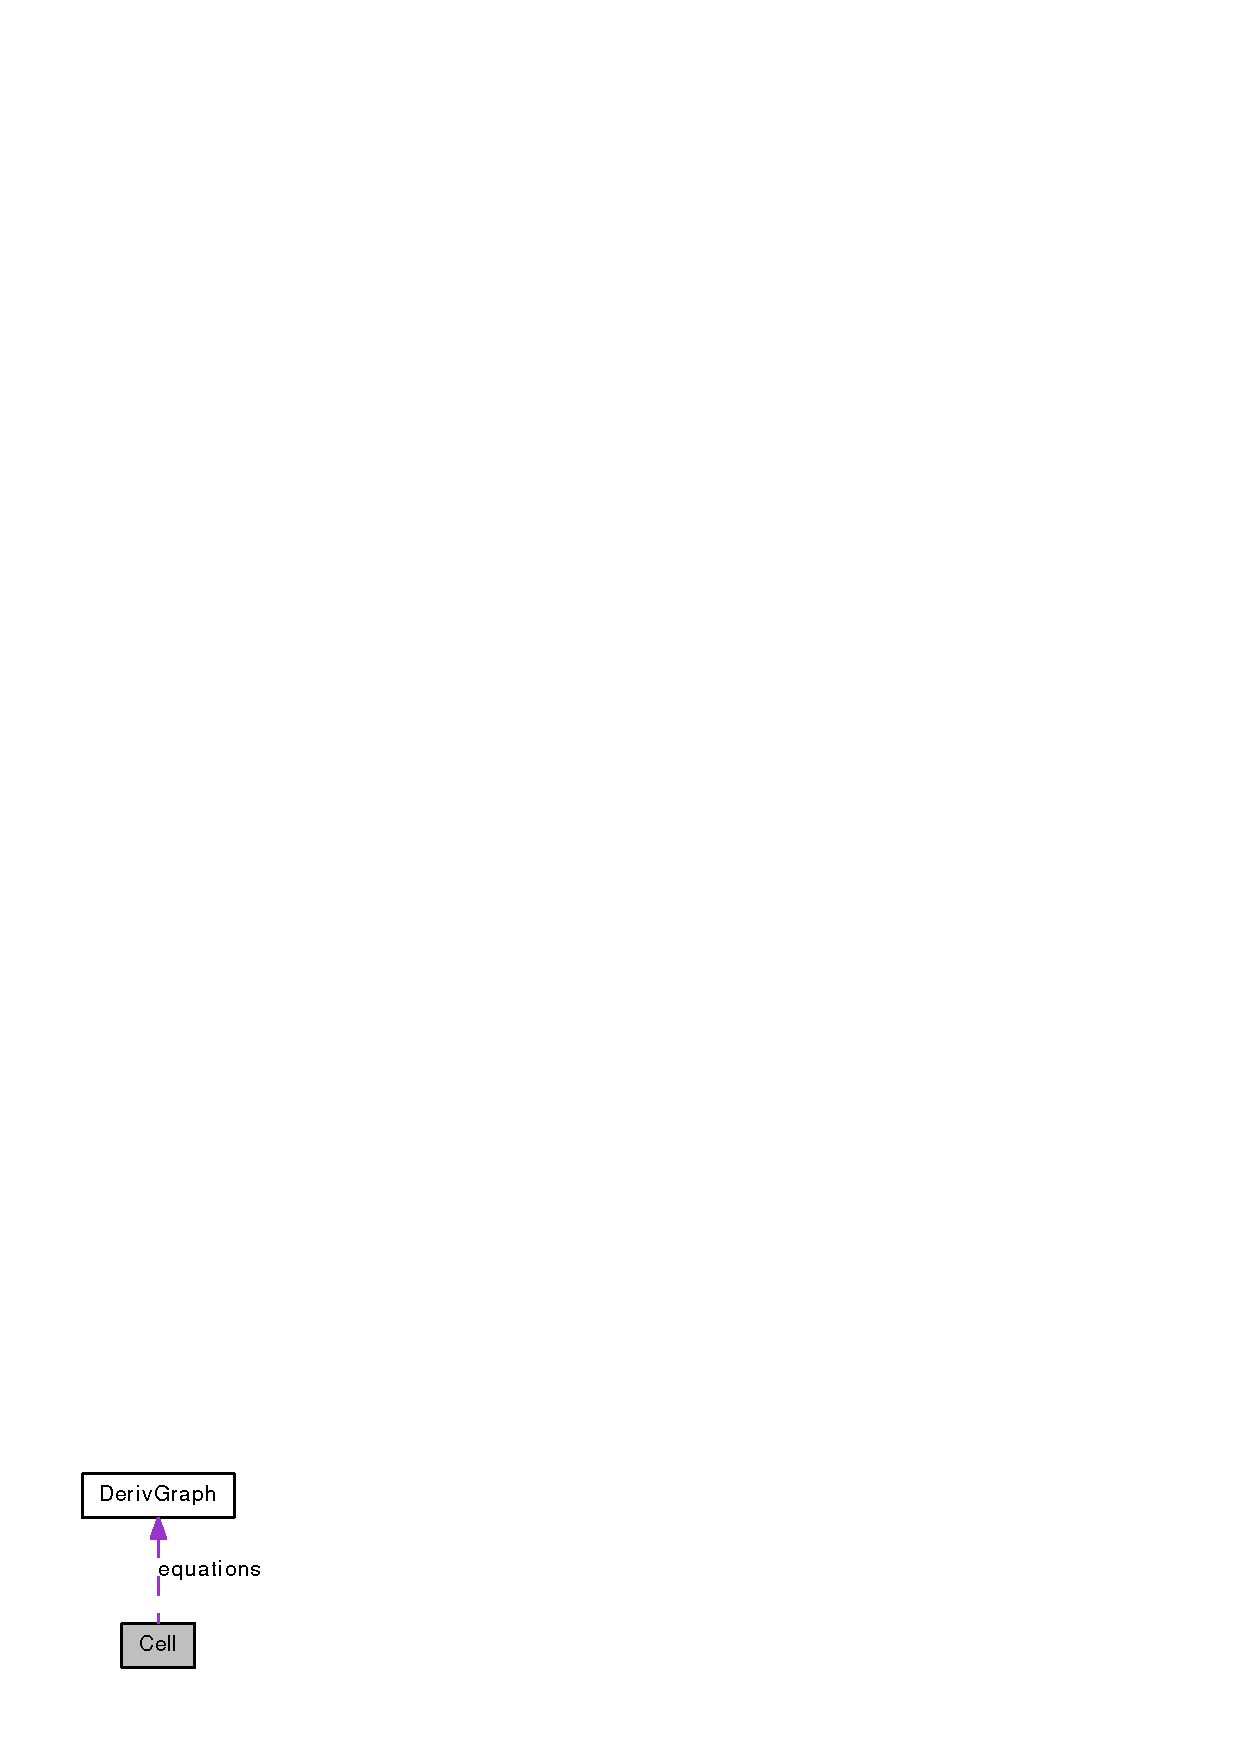
\includegraphics[width=130pt]{classCell__coll__graph}
\end{center}
\end{figure}
\subsection*{Public Member Functions}
\begin{DoxyCompactItemize}
\item 
\hyperlink{classCell_af85b728fb894b346b654eea910958180}{Cell} (int, int, int, int, float, float, float, float, float)
\item 
\hyperlink{classCell_a9fa559f7a28e2b4336c6879ca09304d8}{$\sim$Cell} ()
\item 
int \hyperlink{classCell_a555fa98c5f1dc8d7c88c7a24f69994ff}{mutate} ()
\item 
void \hyperlink{classCell_a535ddddc0471fa874a0b22a54bd38c1a}{outputDotImage} ()
\item 
void \hyperlink{classCell_a8e117526c56dda4d0d56d840d1558835}{outputDataPlot} ()
\item 
int \hyperlink{classCell_a3fbb8b244cc5c516d0728a987d07bf0f}{getScore} ()
\item 
int \hyperlink{classCell_a6fb5e28360b3a6e53400af8b950f6203}{getID} ()
\end{DoxyCompactItemize}


\subsection{Detailed Description}
\hyperlink{classCell}{Cell} header file. 

\subsection{Constructor \& Destructor Documentation}
\hypertarget{classCell_af85b728fb894b346b654eea910958180}{
\index{Cell@{Cell}!Cell@{Cell}}
\index{Cell@{Cell}!Cell@{Cell}}
\subsubsection[{Cell}]{\setlength{\rightskip}{0pt plus 5cm}Cell::Cell (int {\em max\_\-basic}, \/  int {\em max\_\-ptm}, \/  int {\em max\_\-comp}, \/  int {\em max\_\-promoter}, \/  float {\em min\_\-kinetic\_\-rate}, \/  float {\em max\_\-kinetic\_\-rate}, \/  float {\em rk\_\-time\_\-step}, \/  float {\em rk\_\-time\_\-limit}, \/  float {\em initial\_\-conc})}}
\label{classCell_af85b728fb894b346b654eea910958180}
\hyperlink{classCell_af85b728fb894b346b654eea910958180}{Cell::Cell()}

\hyperlink{classCell}{Cell} default constructor.

Allocates: 1 derivGraph object 

Here is the call graph for this function:\nopagebreak
\begin{figure}[H]
\begin{center}
\leavevmode
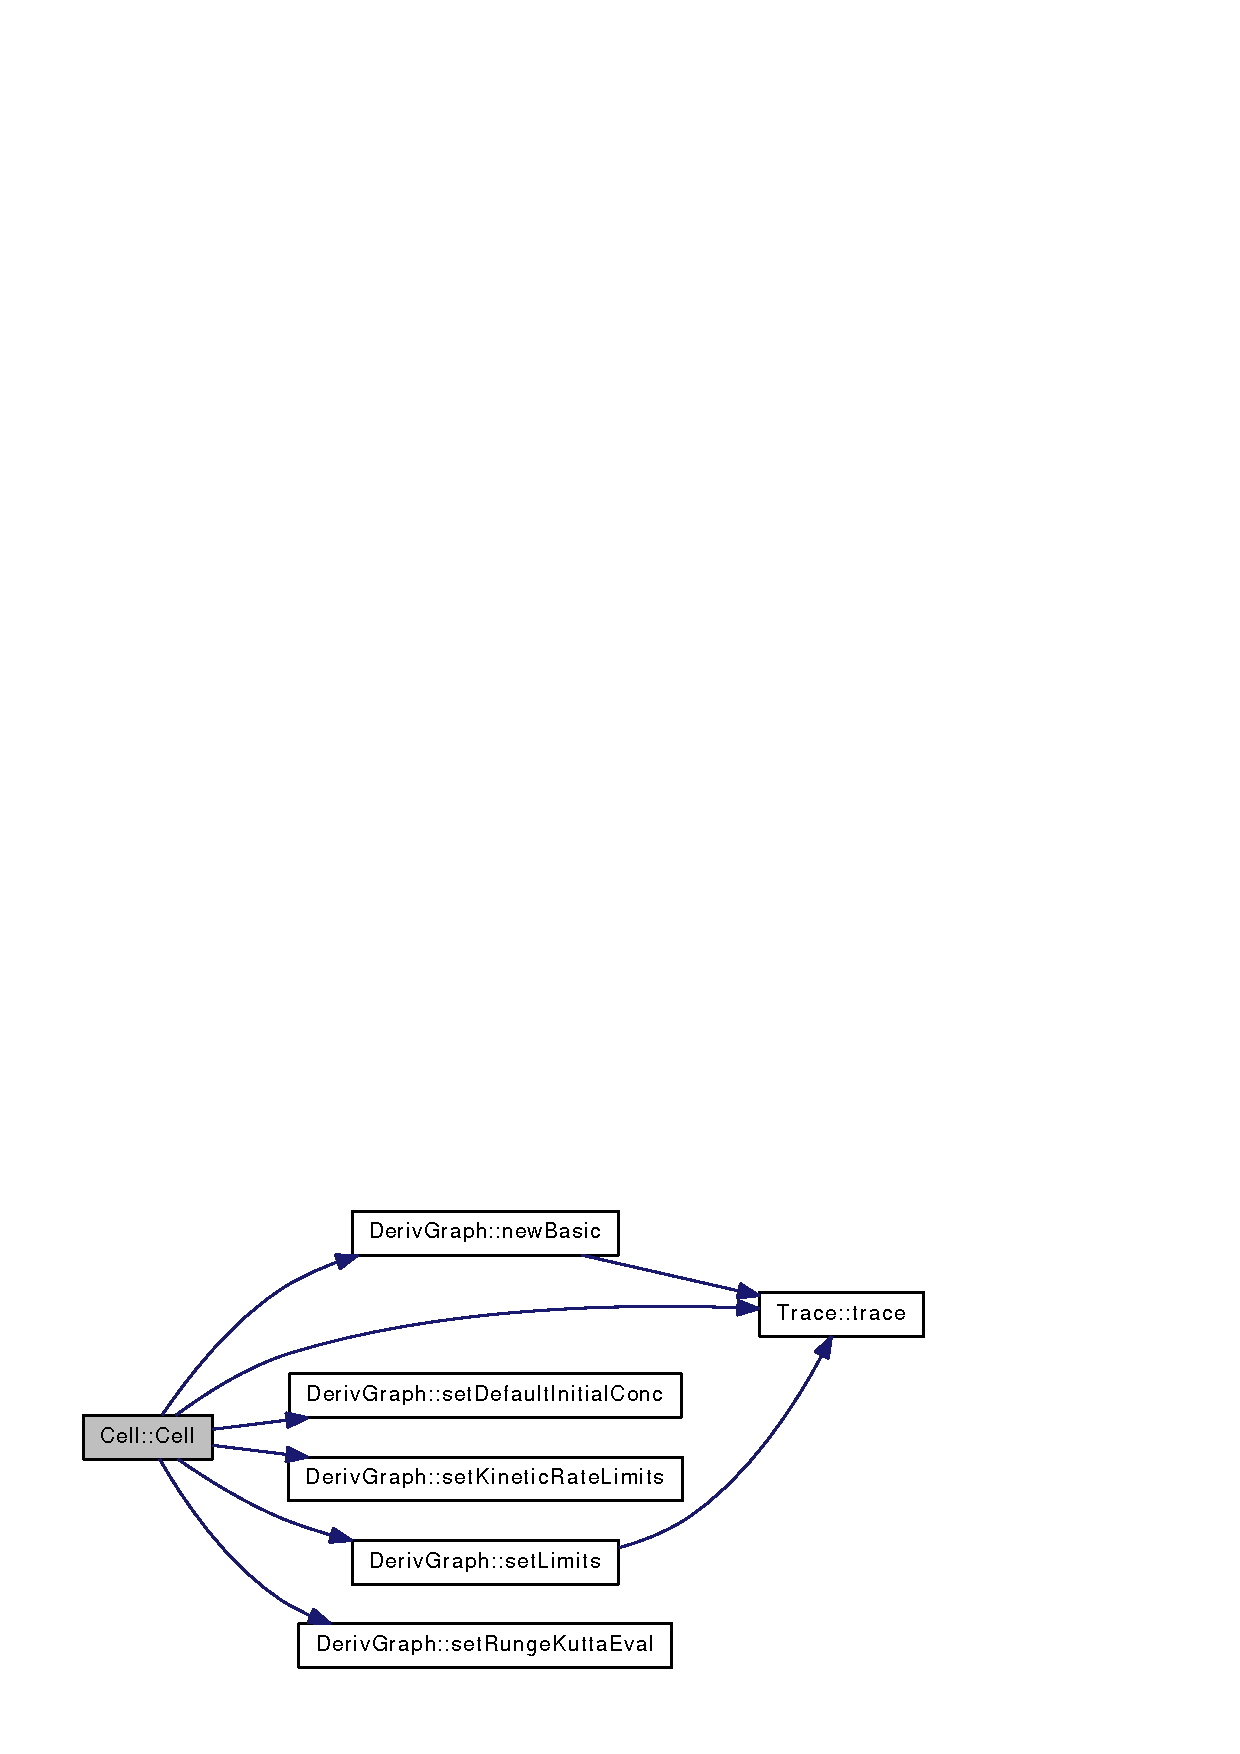
\includegraphics[width=224pt]{classCell_af85b728fb894b346b654eea910958180_cgraph}
\end{center}
\end{figure}
\hypertarget{classCell_a9fa559f7a28e2b4336c6879ca09304d8}{
\index{Cell@{Cell}!$\sim$Cell@{$\sim$Cell}}
\index{$\sim$Cell@{$\sim$Cell}!Cell@{Cell}}
\subsubsection[{$\sim$Cell}]{\setlength{\rightskip}{0pt plus 5cm}Cell::$\sim$Cell ()}}
\label{classCell_a9fa559f7a28e2b4336c6879ca09304d8}
\hyperlink{classCell_a9fa559f7a28e2b4336c6879ca09304d8}{Cell::$\sim$Cell()}

\hyperlink{classCell}{Cell} default destructor.

Frees: 1 derivGraph object 

Here is the call graph for this function:\nopagebreak
\begin{figure}[H]
\begin{center}
\leavevmode
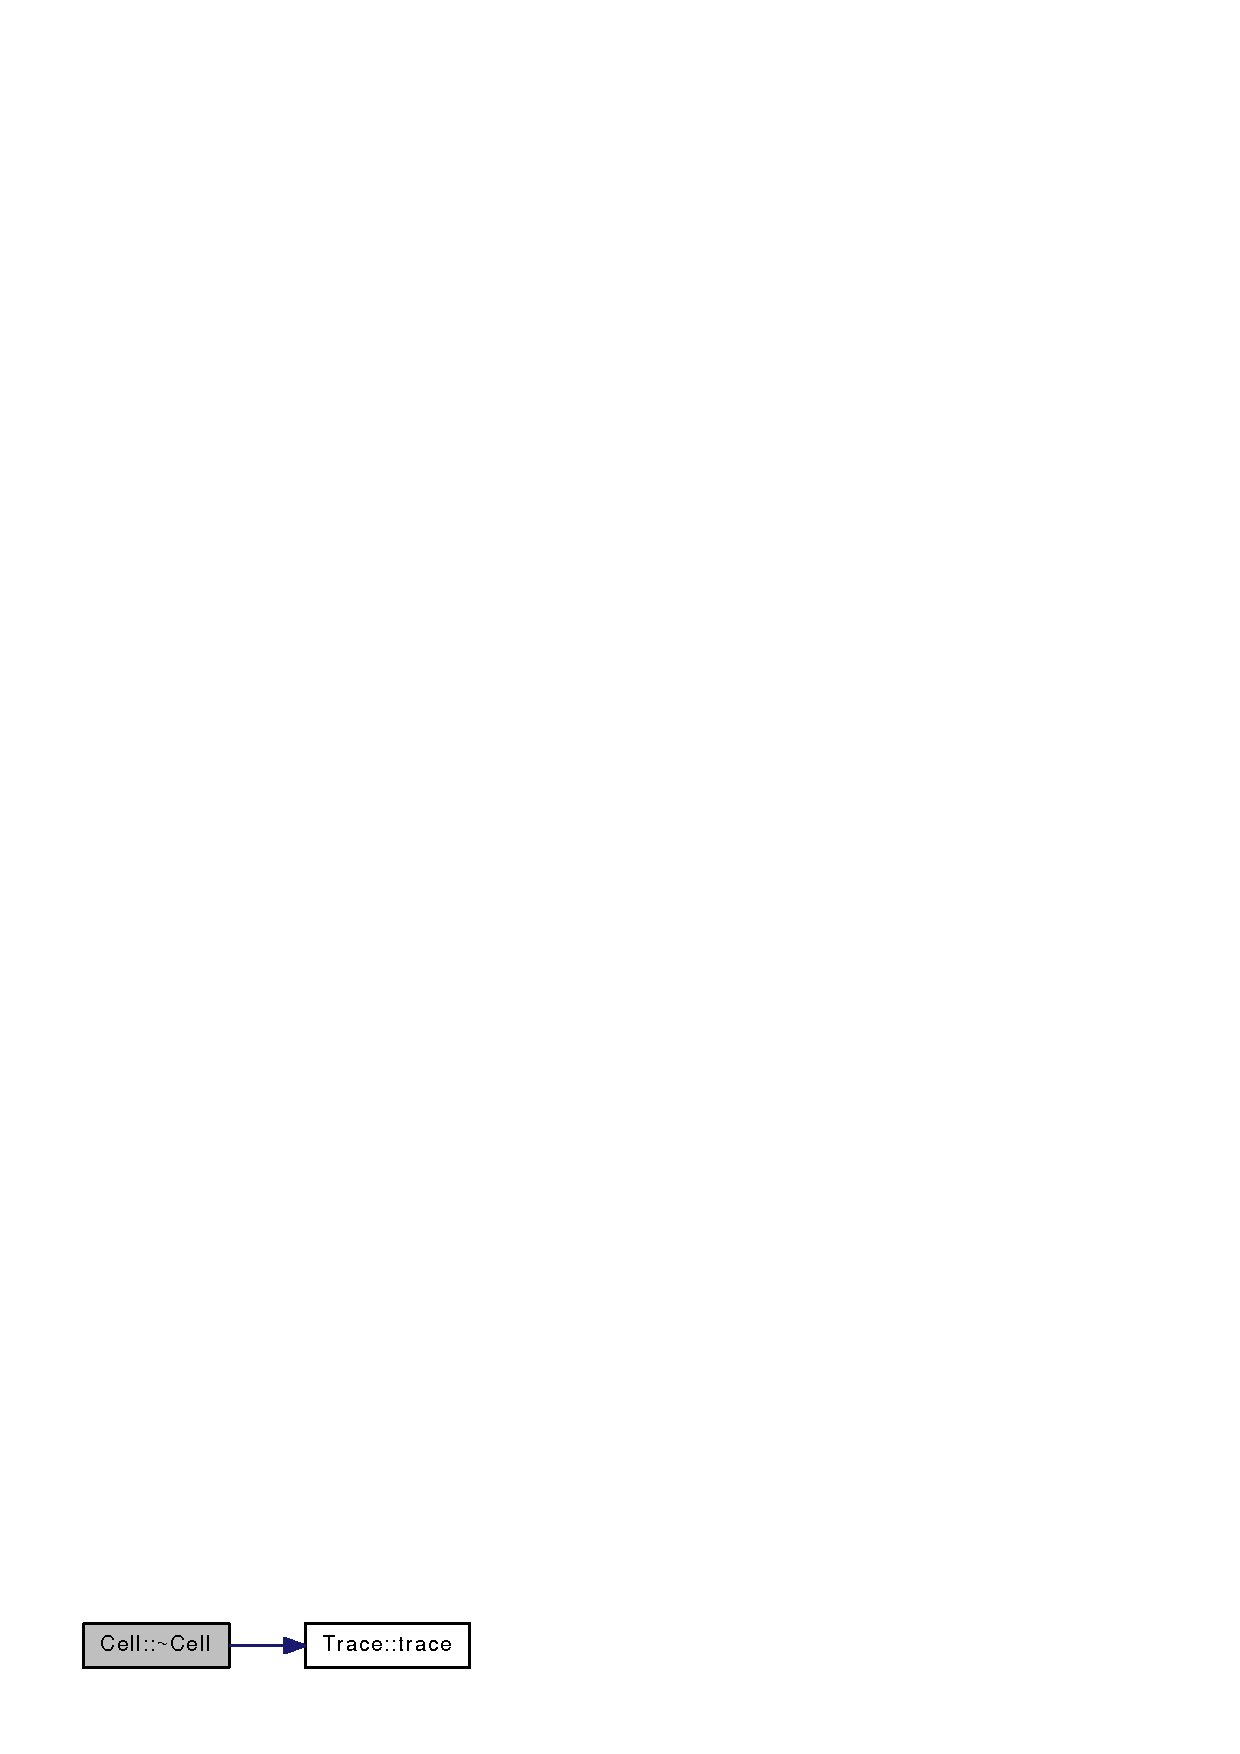
\includegraphics[width=115pt]{classCell_a9fa559f7a28e2b4336c6879ca09304d8_cgraph}
\end{center}
\end{figure}


\subsection{Member Function Documentation}
\hypertarget{classCell_a6fb5e28360b3a6e53400af8b950f6203}{
\index{Cell@{Cell}!getID@{getID}}
\index{getID@{getID}!Cell@{Cell}}
\subsubsection[{getID}]{\setlength{\rightskip}{0pt plus 5cm}int Cell::getID ()\hspace{0.3cm}{\ttfamily  \mbox{[}inline\mbox{]}}}}
\label{classCell_a6fb5e28360b3a6e53400af8b950f6203}
\hypertarget{classCell_a3fbb8b244cc5c516d0728a987d07bf0f}{
\index{Cell@{Cell}!getScore@{getScore}}
\index{getScore@{getScore}!Cell@{Cell}}
\subsubsection[{getScore}]{\setlength{\rightskip}{0pt plus 5cm}int Cell::getScore ()}}
\label{classCell_a3fbb8b244cc5c516d0728a987d07bf0f}


Here is the call graph for this function:\nopagebreak
\begin{figure}[H]
\begin{center}
\leavevmode
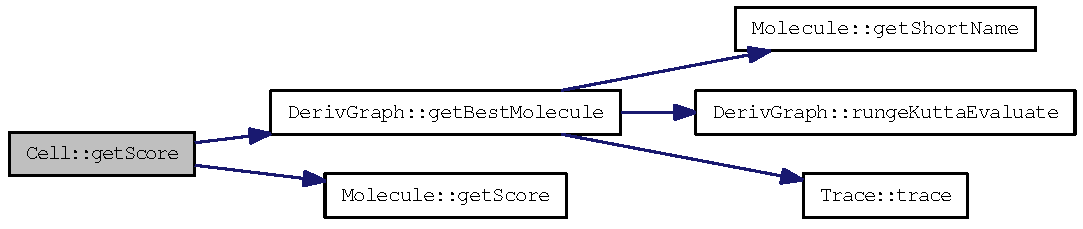
\includegraphics[width=259pt]{classCell_a3fbb8b244cc5c516d0728a987d07bf0f_cgraph}
\end{center}
\end{figure}
\hypertarget{classCell_a555fa98c5f1dc8d7c88c7a24f69994ff}{
\index{Cell@{Cell}!mutate@{mutate}}
\index{mutate@{mutate}!Cell@{Cell}}
\subsubsection[{mutate}]{\setlength{\rightskip}{0pt plus 5cm}int Cell::mutate ()}}
\label{classCell_a555fa98c5f1dc8d7c88c7a24f69994ff}


Here is the call graph for this function:\nopagebreak
\begin{figure}[H]
\begin{center}
\leavevmode
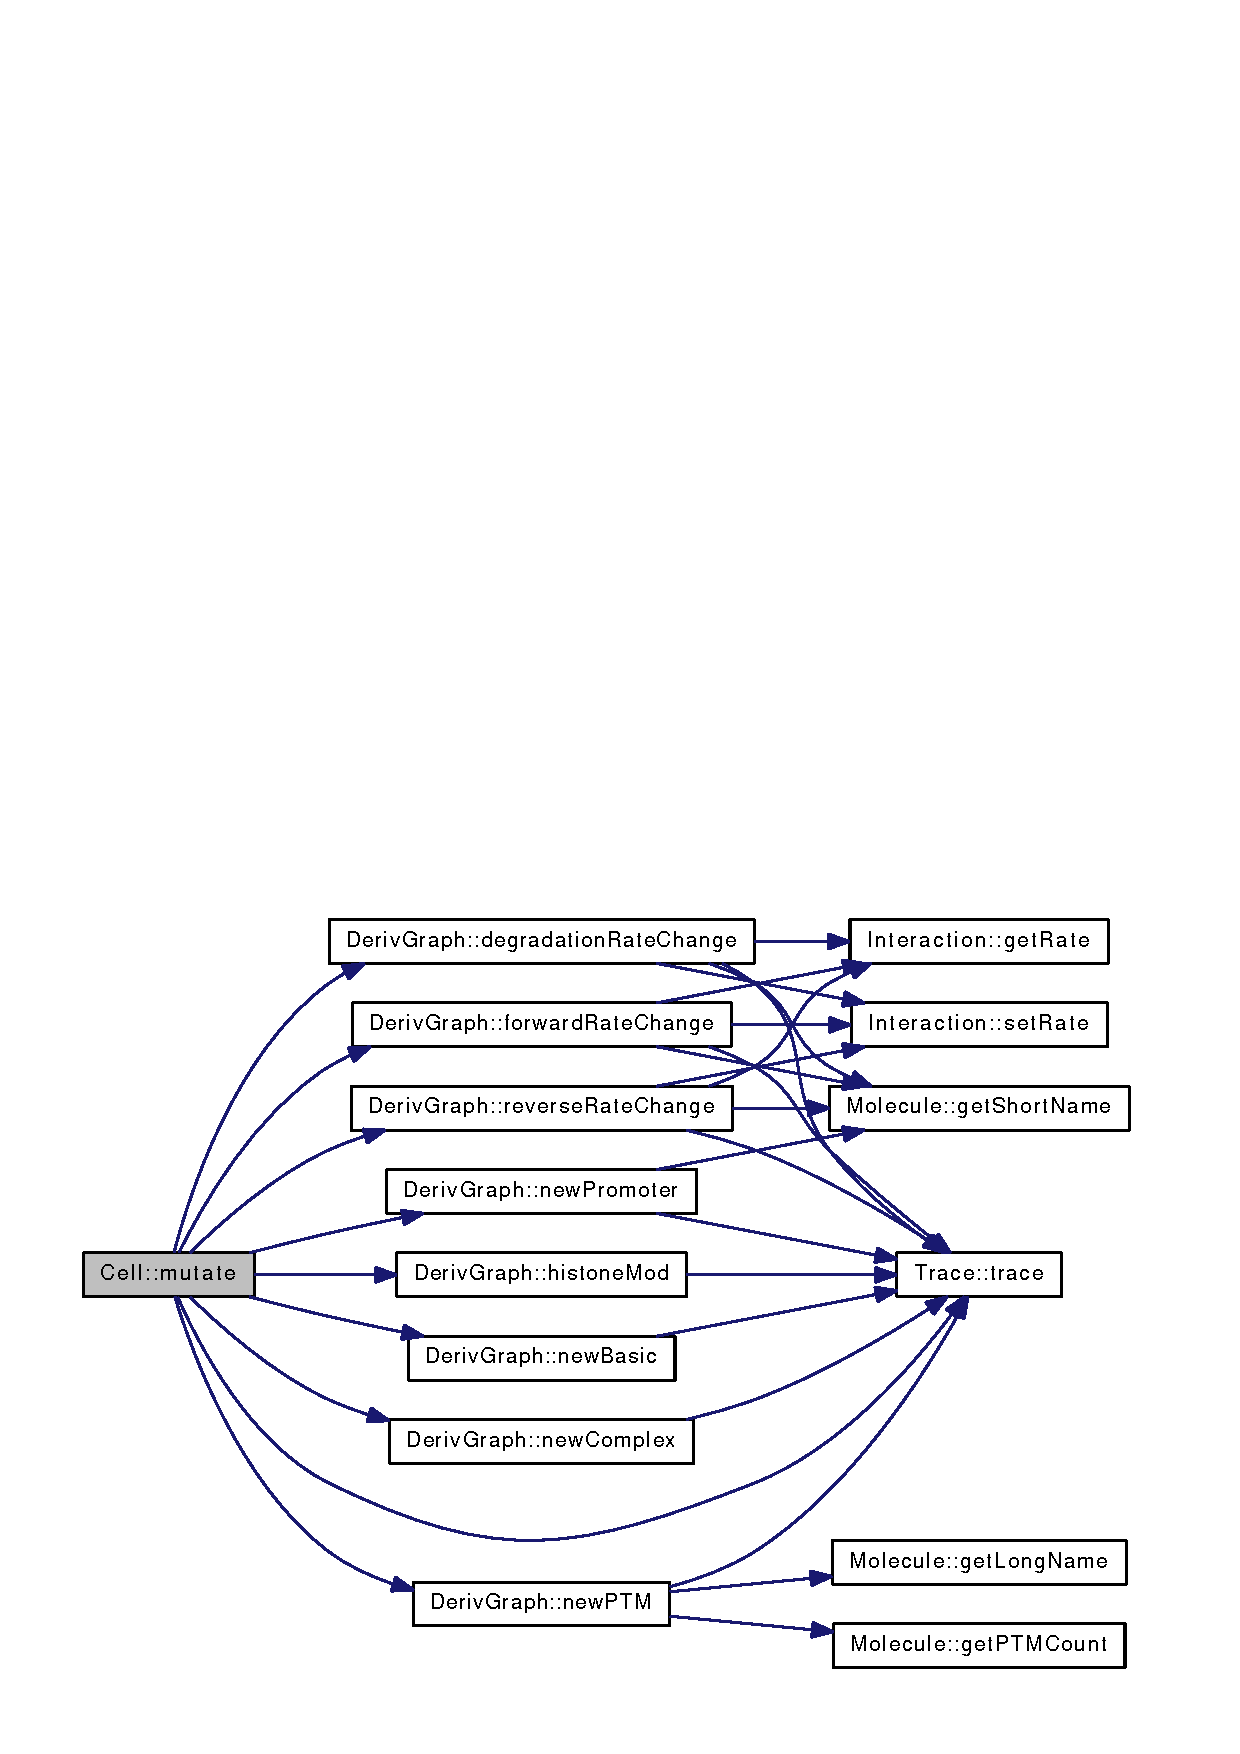
\includegraphics[width=273pt]{classCell_a555fa98c5f1dc8d7c88c7a24f69994ff_cgraph}
\end{center}
\end{figure}
\hypertarget{classCell_a8e117526c56dda4d0d56d840d1558835}{
\index{Cell@{Cell}!outputDataPlot@{outputDataPlot}}
\index{outputDataPlot@{outputDataPlot}!Cell@{Cell}}
\subsubsection[{outputDataPlot}]{\setlength{\rightskip}{0pt plus 5cm}void Cell::outputDataPlot ()}}
\label{classCell_a8e117526c56dda4d0d56d840d1558835}


Here is the call graph for this function:\nopagebreak
\begin{figure}[H]
\begin{center}
\leavevmode
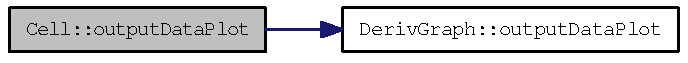
\includegraphics[width=183pt]{classCell_a8e117526c56dda4d0d56d840d1558835_cgraph}
\end{center}
\end{figure}
\hypertarget{classCell_a535ddddc0471fa874a0b22a54bd38c1a}{
\index{Cell@{Cell}!outputDotImage@{outputDotImage}}
\index{outputDotImage@{outputDotImage}!Cell@{Cell}}
\subsubsection[{outputDotImage}]{\setlength{\rightskip}{0pt plus 5cm}void Cell::outputDotImage ()}}
\label{classCell_a535ddddc0471fa874a0b22a54bd38c1a}


Here is the call graph for this function:\nopagebreak
\begin{figure}[H]
\begin{center}
\leavevmode
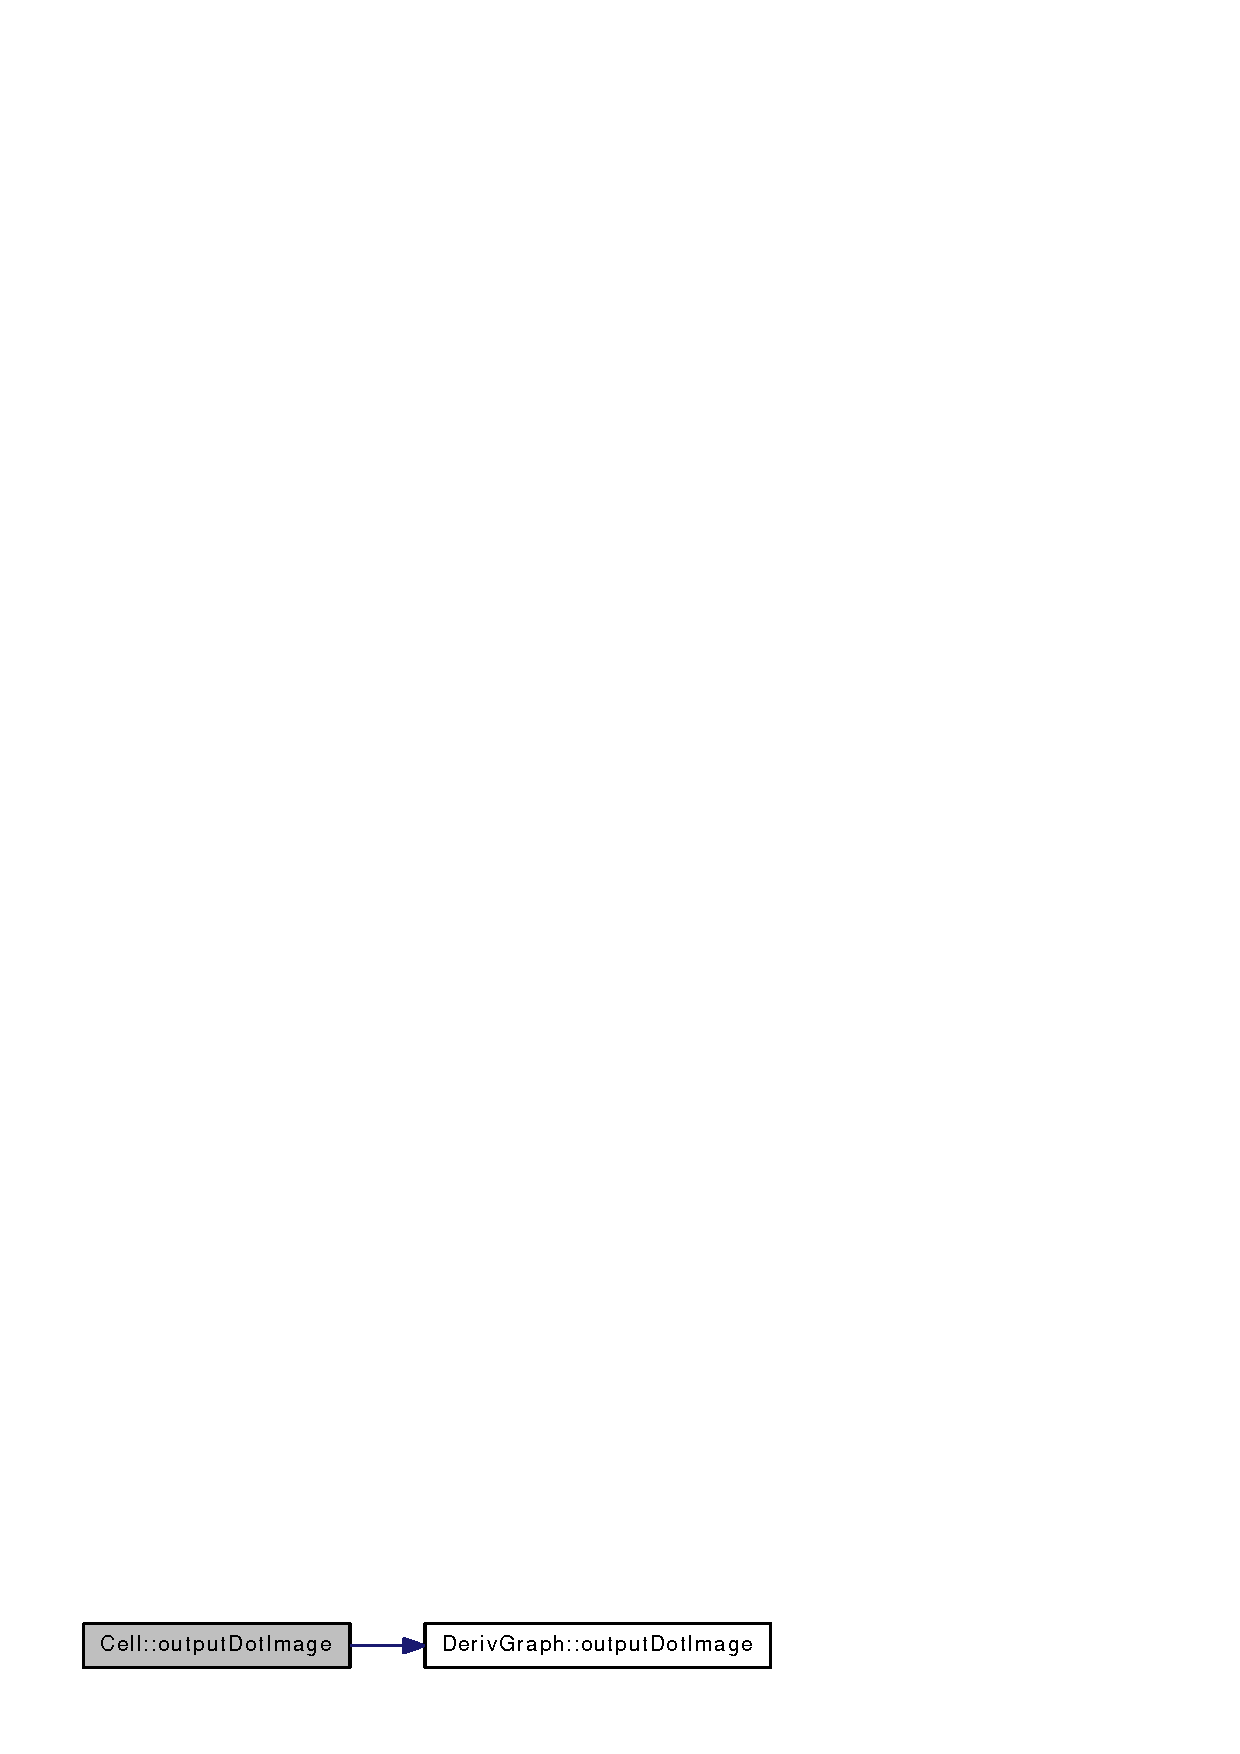
\includegraphics[width=187pt]{classCell_a535ddddc0471fa874a0b22a54bd38c1a_cgraph}
\end{center}
\end{figure}


The documentation for this class was generated from the following files:\begin{DoxyCompactItemize}
\item 
\hyperlink{Cell_8h}{Cell.h}\item 
\hyperlink{Cell_8cpp}{Cell.cpp}\end{DoxyCompactItemize}

\hypertarget{structcmp__str}{
\section{cmp\_\-str Struct Reference}
\label{structcmp__str}\index{cmp\_\-str@{cmp\_\-str}}
}


{\ttfamily \#include $<$Trace.h$>$}\subsection*{Public Member Functions}
\begin{DoxyCompactItemize}
\item 
bool \hyperlink{structcmp__str_a2372a37bf9dcd1b9bcd95583e20cc058}{operator()} (const char $\ast$a, const char $\ast$b)
\end{DoxyCompactItemize}


\subsection{Member Function Documentation}
\hypertarget{structcmp__str_a2372a37bf9dcd1b9bcd95583e20cc058}{
\index{cmp\_\-str@{cmp\_\-str}!operator()@{operator()}}
\index{operator()@{operator()}!cmp_str@{cmp\_\-str}}
\subsubsection[{operator()}]{\setlength{\rightskip}{0pt plus 5cm}bool cmp\_\-str::operator() (const char $\ast$ {\em a}, \/  const char $\ast$ {\em b})\hspace{0.3cm}{\ttfamily  \mbox{[}inline\mbox{]}}}}
\label{structcmp__str_a2372a37bf9dcd1b9bcd95583e20cc058}


The documentation for this struct was generated from the following file:\begin{DoxyCompactItemize}
\item 
\hyperlink{Trace_8h}{Trace.h}\end{DoxyCompactItemize}

\hypertarget{classComplex}{
\section{Complex Class Reference}
\label{classComplex}\index{Complex@{Complex}}
}


{\ttfamily \#include $<$CustomMolecules.h$>$}Inheritance diagram for Complex:\nopagebreak
\begin{figure}[H]
\begin{center}
\leavevmode
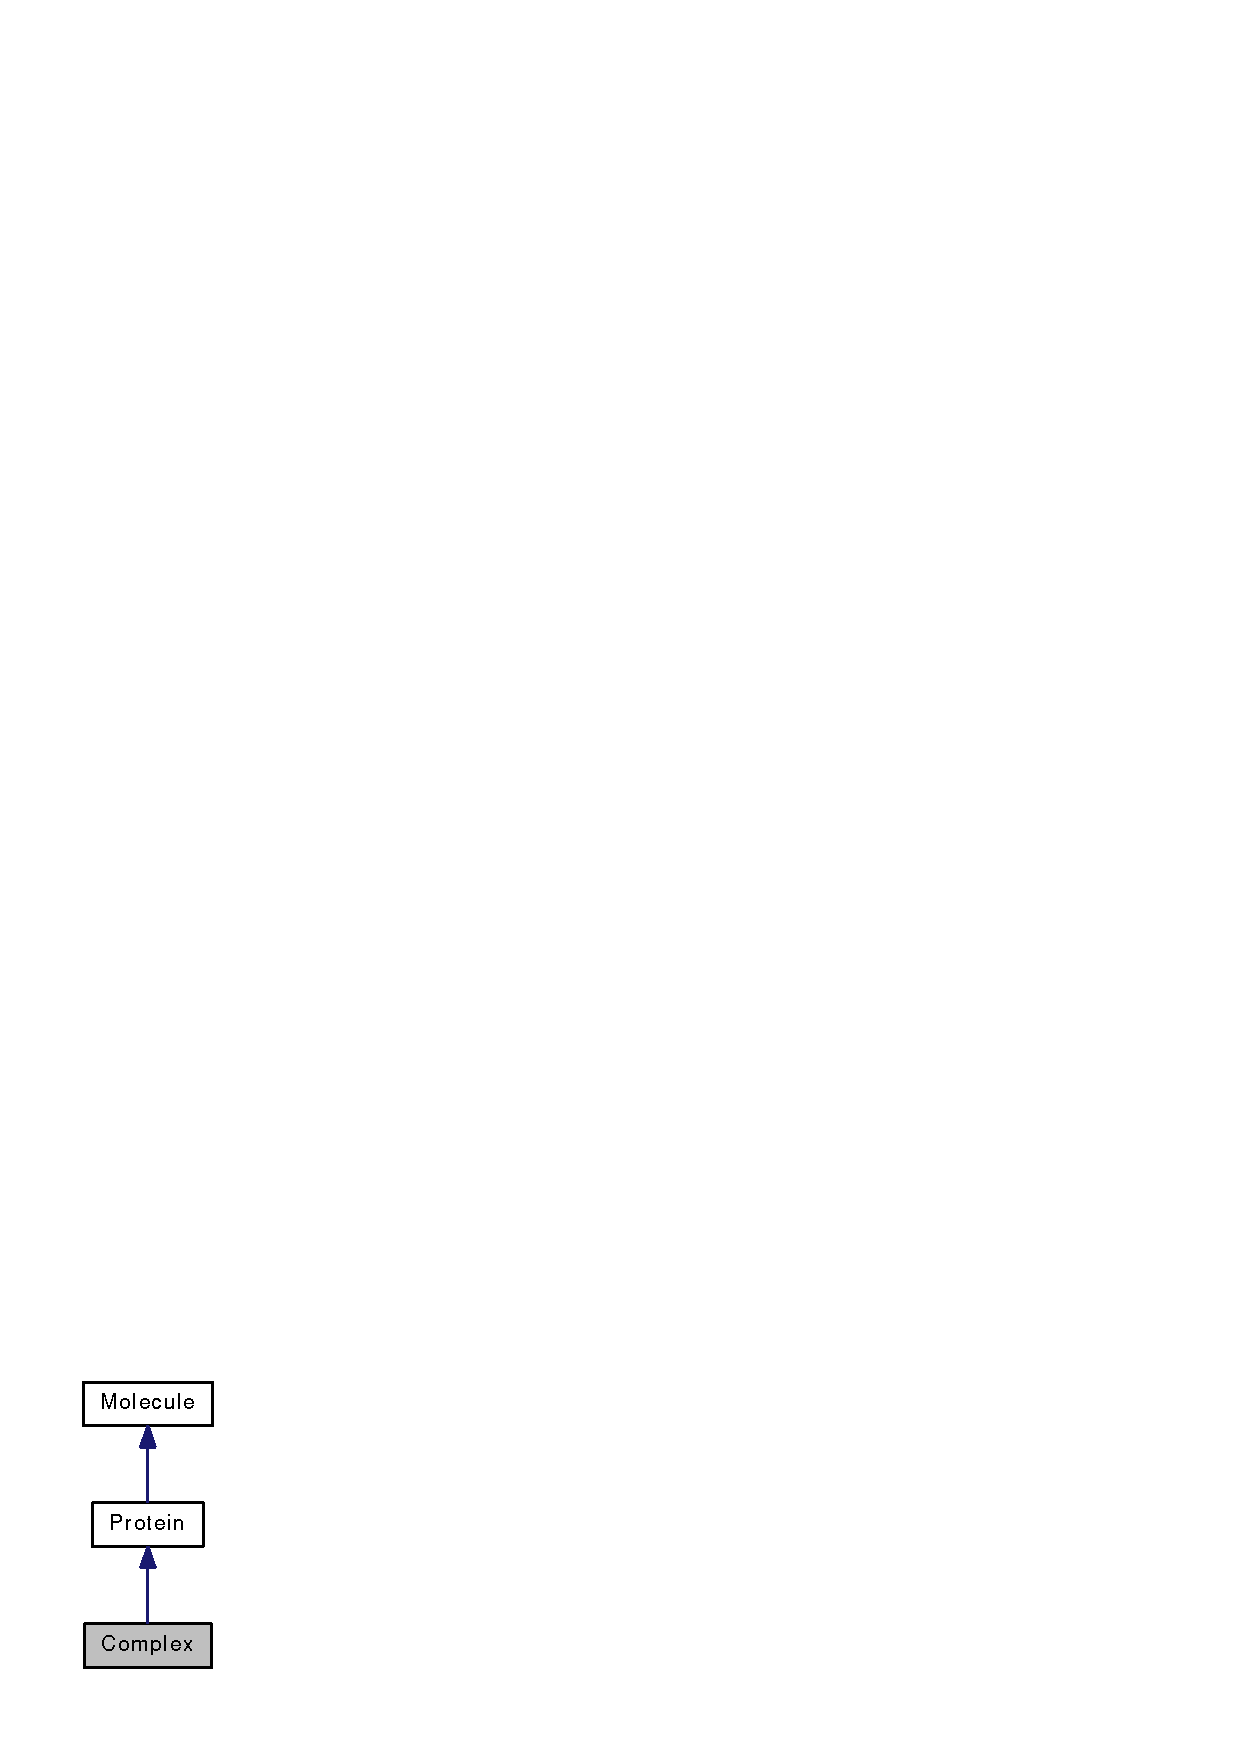
\includegraphics[width=106pt]{classComplex__inherit__graph}
\end{center}
\end{figure}
Collaboration diagram for Complex:\nopagebreak
\begin{figure}[H]
\begin{center}
\leavevmode
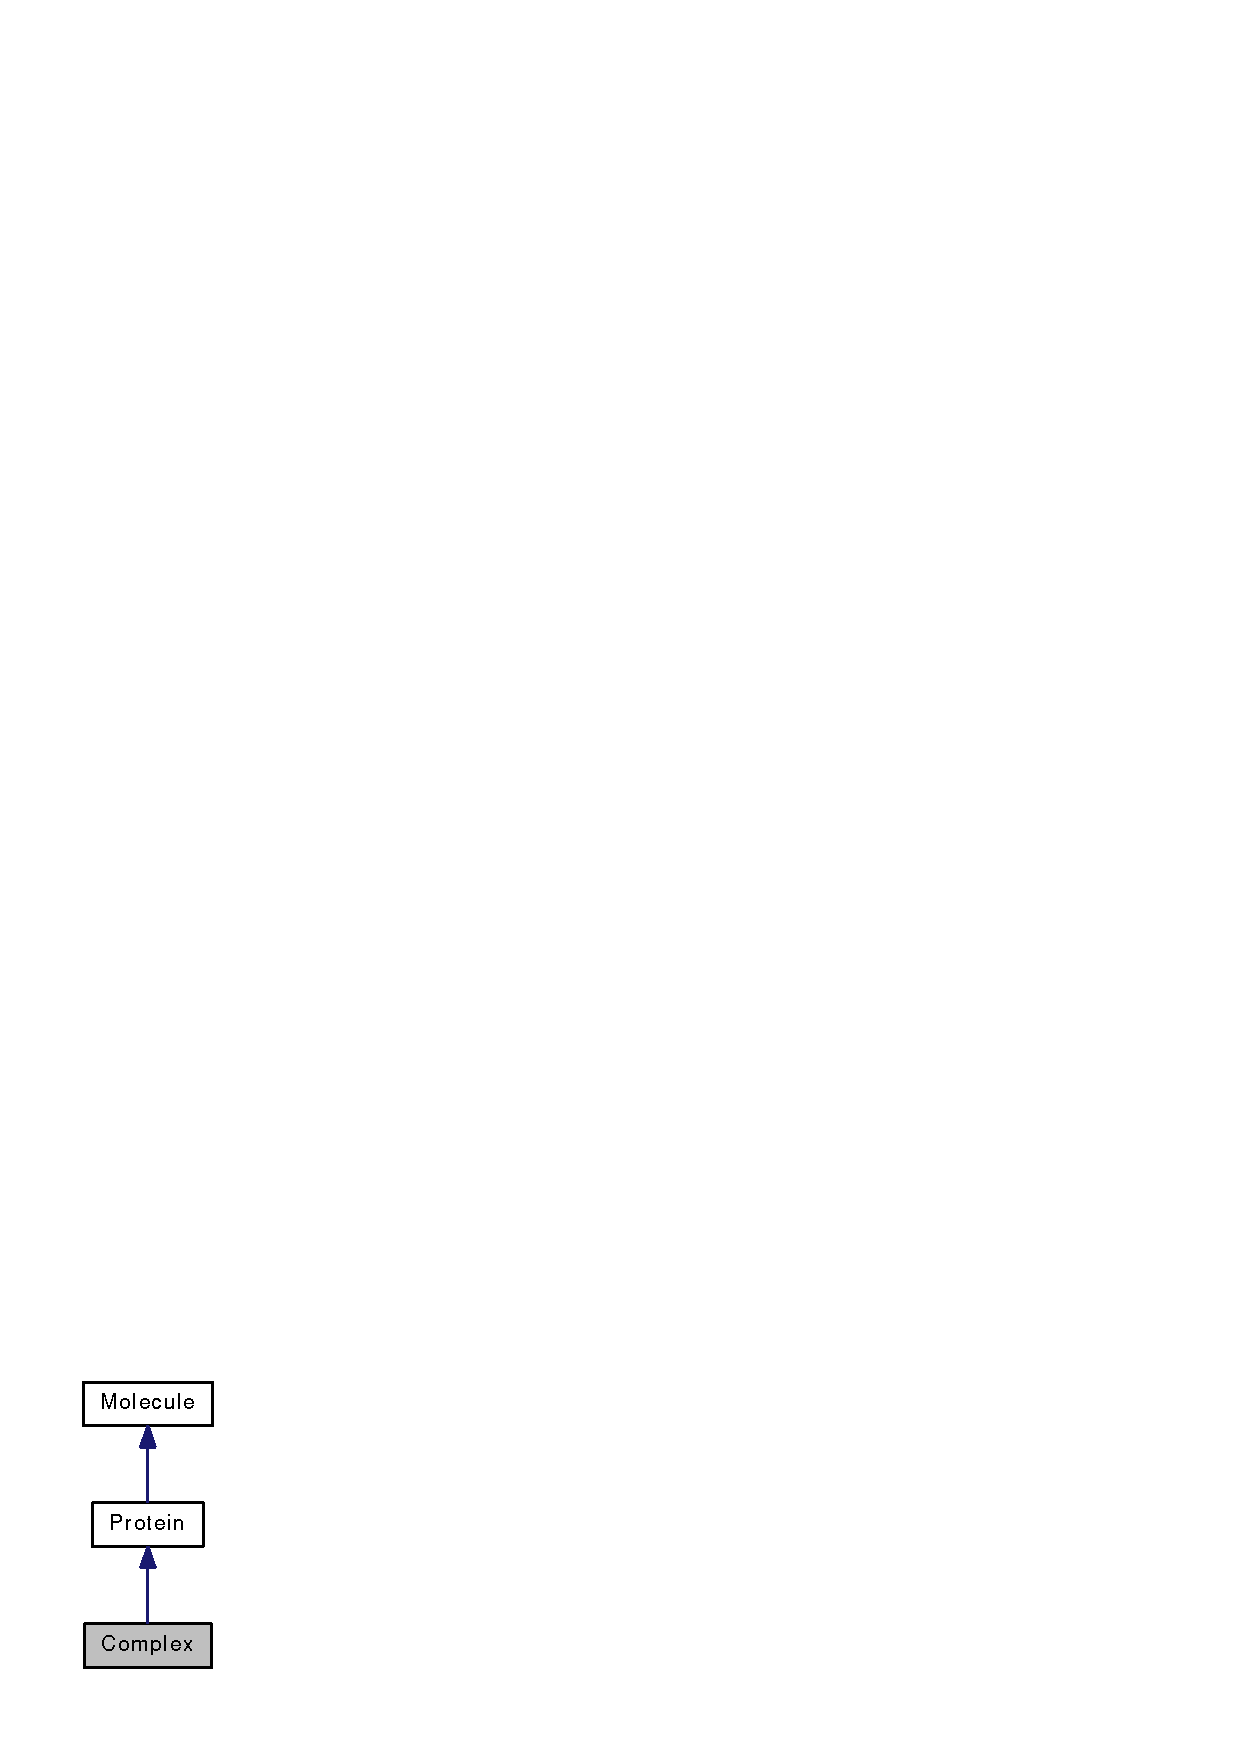
\includegraphics[width=106pt]{classComplex__coll__graph}
\end{center}
\end{figure}
\subsection*{Public Member Functions}
\begin{DoxyCompactItemize}
\item 
\hyperlink{classComplex_ad551ee48d65fa588fdaea8d5dd3f565c}{Complex} (int, int)
\item 
\hyperlink{classComplex_a70e14b17c92e3da779686b98f9f3bb2d}{$\sim$Complex} ()
\item 
int \hyperlink{classComplex_a87fc032569ab11bdf80a5ac3cabfd2fc}{getComponentId} (int)
\end{DoxyCompactItemize}


\subsection{Constructor \& Destructor Documentation}
\hypertarget{classComplex_ad551ee48d65fa588fdaea8d5dd3f565c}{
\index{Complex@{Complex}!Complex@{Complex}}
\index{Complex@{Complex}!Complex@{Complex}}
\subsubsection[{Complex}]{\setlength{\rightskip}{0pt plus 5cm}Complex::Complex (int {\em n1}, \/  int {\em n2})}}
\label{classComplex_ad551ee48d65fa588fdaea8d5dd3f565c}


Here is the call graph for this function:\nopagebreak
\begin{figure}[H]
\begin{center}
\leavevmode
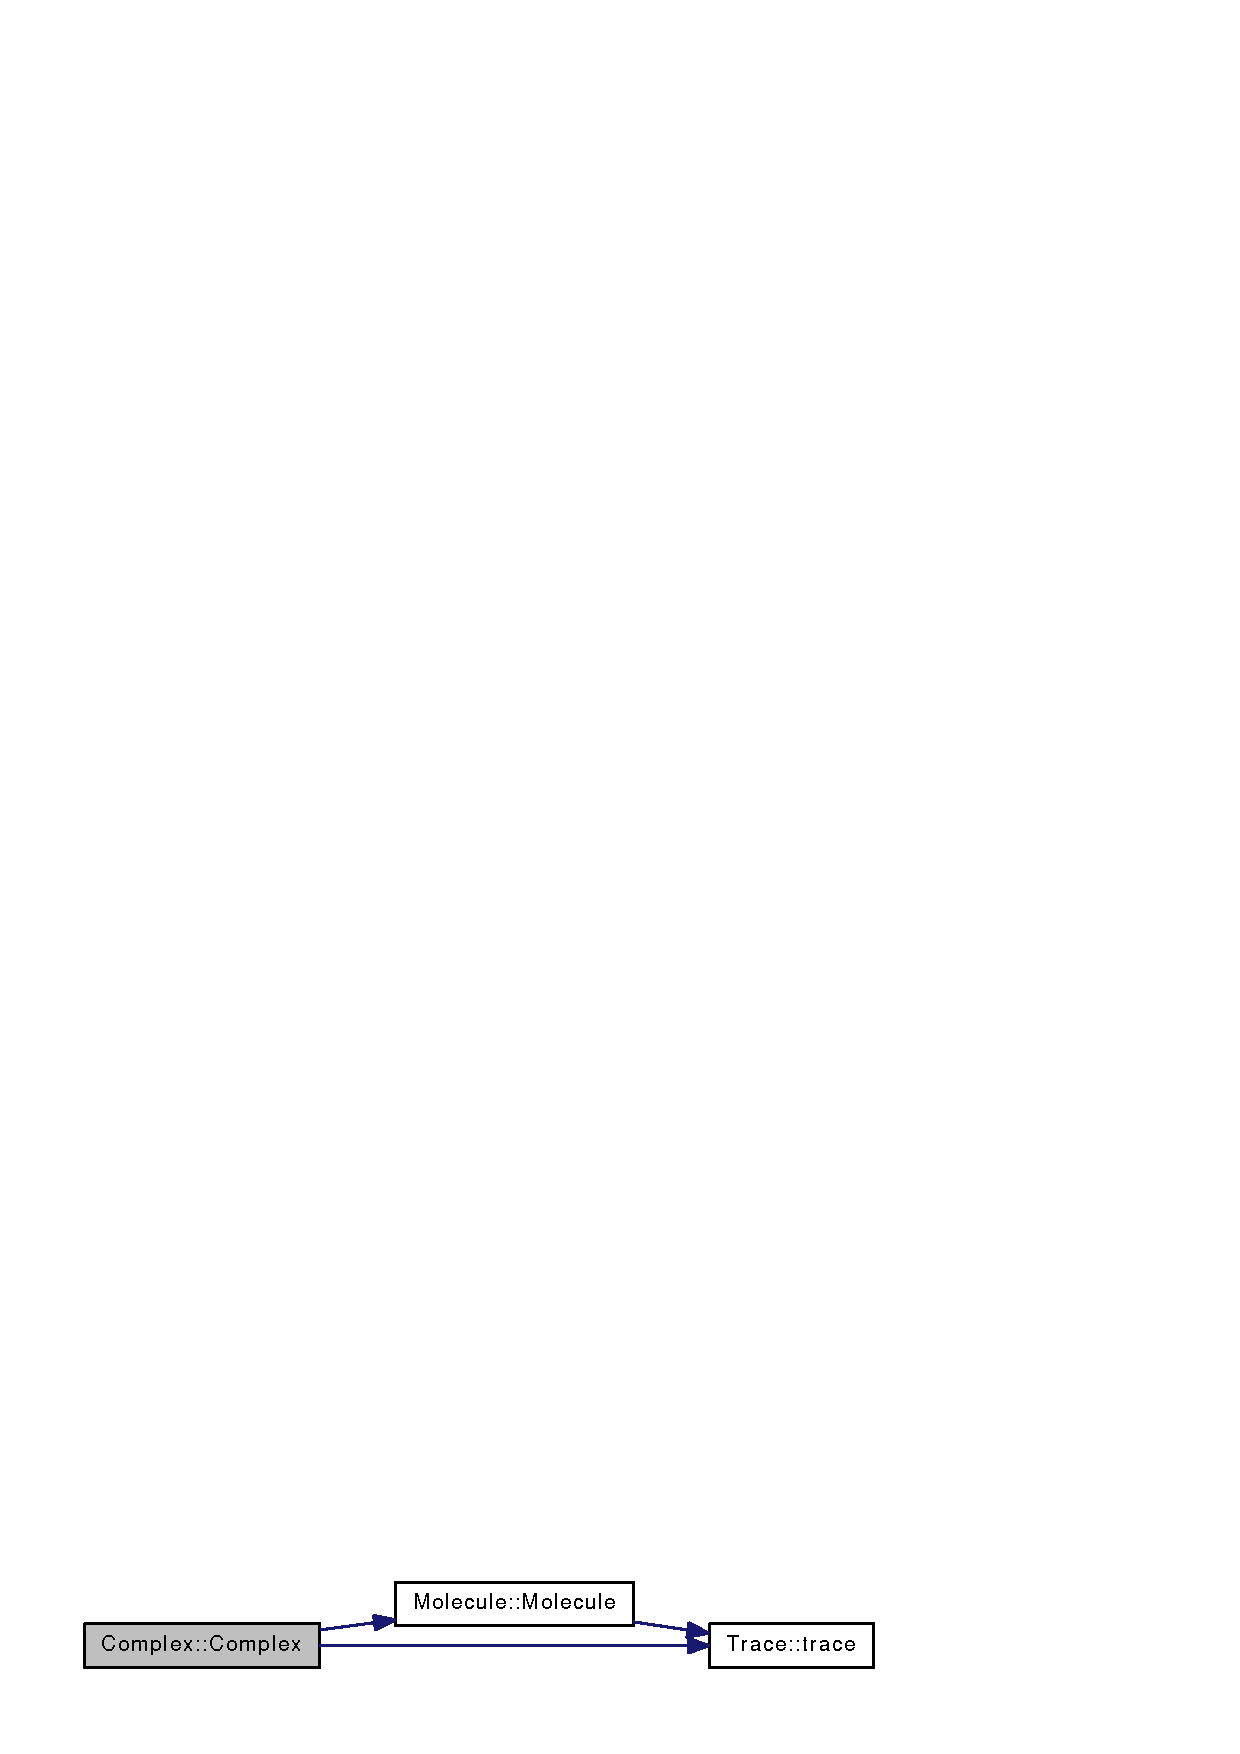
\includegraphics[width=212pt]{classComplex_ad551ee48d65fa588fdaea8d5dd3f565c_cgraph}
\end{center}
\end{figure}
\hypertarget{classComplex_a70e14b17c92e3da779686b98f9f3bb2d}{
\index{Complex@{Complex}!$\sim$Complex@{$\sim$Complex}}
\index{$\sim$Complex@{$\sim$Complex}!Complex@{Complex}}
\subsubsection[{$\sim$Complex}]{\setlength{\rightskip}{0pt plus 5cm}Complex::$\sim$Complex ()}}
\label{classComplex_a70e14b17c92e3da779686b98f9f3bb2d}


\subsection{Member Function Documentation}
\hypertarget{classComplex_a87fc032569ab11bdf80a5ac3cabfd2fc}{
\index{Complex@{Complex}!getComponentId@{getComponentId}}
\index{getComponentId@{getComponentId}!Complex@{Complex}}
\subsubsection[{getComponentId}]{\setlength{\rightskip}{0pt plus 5cm}int Complex::getComponentId (int {\em i})}}
\label{classComplex_a87fc032569ab11bdf80a5ac3cabfd2fc}


The documentation for this class was generated from the following files:\begin{DoxyCompactItemize}
\item 
\hyperlink{CustomMolecules_8h}{CustomMolecules.h}\item 
\hyperlink{CustomMolecules_8cpp}{CustomMolecules.cpp}\end{DoxyCompactItemize}

\hypertarget{classDegradation}{
\section{Degradation Class Reference}
\label{classDegradation}\index{Degradation@{Degradation}}
}


{\ttfamily \#include $<$CustomInteractions.h$>$}Inheritance diagram for Degradation:\nopagebreak
\begin{figure}[H]
\begin{center}
\leavevmode
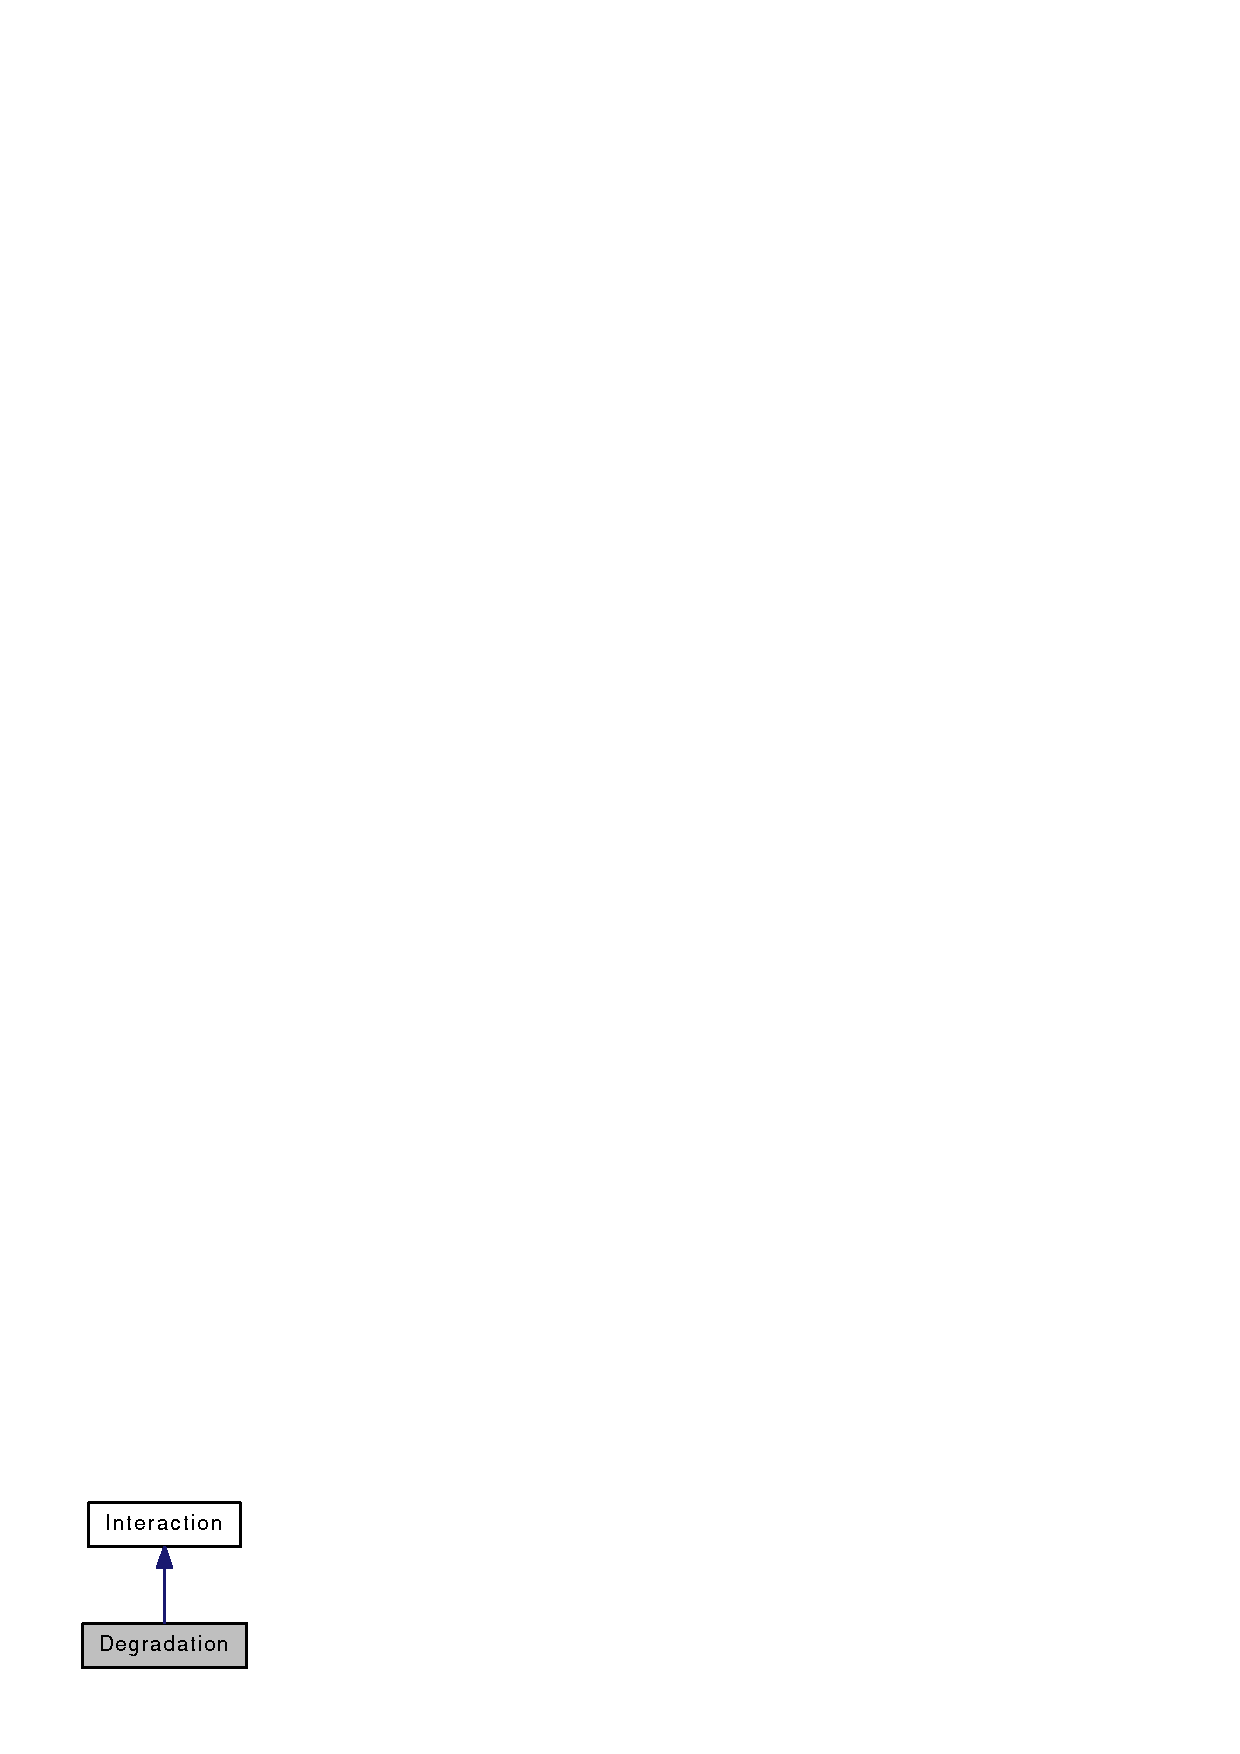
\includegraphics[width=122pt]{classDegradation__inherit__graph}
\end{center}
\end{figure}
Collaboration diagram for Degradation:\nopagebreak
\begin{figure}[H]
\begin{center}
\leavevmode
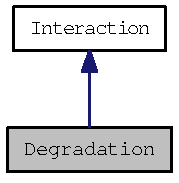
\includegraphics[width=122pt]{classDegradation__coll__graph}
\end{center}
\end{figure}
\subsection*{Public Member Functions}
\begin{DoxyCompactItemize}
\item 
\hyperlink{classDegradation_a1a703897347e37fd019c8ad9ff033d17}{Degradation} ()
\item 
\hyperlink{classDegradation_adb12186e524e71c1d633e6ccfb09e322}{$\sim$Degradation} ()
\item 
virtual float \hyperlink{classDegradation_a3cad4fc84026c6f627306a7e35527f3c}{getEffect} (ListDigraph $\ast$, ListDigraph::NodeMap$<$ \hyperlink{classMolecule}{Molecule} $\ast$ $>$ $\ast$, ListDigraph::ArcMap$<$ \hyperlink{classInteraction}{Interaction} $\ast$ $>$ $\ast$, ListDigraph::Node, int, float)
\end{DoxyCompactItemize}


\subsection{Constructor \& Destructor Documentation}
\hypertarget{classDegradation_a1a703897347e37fd019c8ad9ff033d17}{
\index{Degradation@{Degradation}!Degradation@{Degradation}}
\index{Degradation@{Degradation}!Degradation@{Degradation}}
\subsubsection[{Degradation}]{\setlength{\rightskip}{0pt plus 5cm}Degradation::Degradation ()}}
\label{classDegradation_a1a703897347e37fd019c8ad9ff033d17}
\hypertarget{classDegradation_adb12186e524e71c1d633e6ccfb09e322}{
\index{Degradation@{Degradation}!$\sim$Degradation@{$\sim$Degradation}}
\index{$\sim$Degradation@{$\sim$Degradation}!Degradation@{Degradation}}
\subsubsection[{$\sim$Degradation}]{\setlength{\rightskip}{0pt plus 5cm}Degradation::$\sim$Degradation ()}}
\label{classDegradation_adb12186e524e71c1d633e6ccfb09e322}


\subsection{Member Function Documentation}
\hypertarget{classDegradation_a3cad4fc84026c6f627306a7e35527f3c}{
\index{Degradation@{Degradation}!getEffect@{getEffect}}
\index{getEffect@{getEffect}!Degradation@{Degradation}}
\subsubsection[{getEffect}]{\setlength{\rightskip}{0pt plus 5cm}float Degradation::getEffect (ListDigraph $\ast$ {\em g}, \/  ListDigraph::NodeMap$<$ {\bf Molecule} $\ast$ $>$ $\ast$ {\em m}, \/  ListDigraph::ArcMap$<$ {\bf Interaction} $\ast$ $>$ $\ast$ {\em i}, \/  ListDigraph::Node {\em a}, \/  int {\em rkIter}, \/  float {\em rkStep})\hspace{0.3cm}{\ttfamily  \mbox{[}virtual\mbox{]}}}}
\label{classDegradation_a3cad4fc84026c6f627306a7e35527f3c}
float Interaction::getEffect(ListDigraph$\ast$ , NodeMap$<$Molecule$\ast$$>$$\ast$ , ArcMap$<$Interaction$\ast$$>$$\ast$ , Node , int, float)

Get the effect this interaction has on a particular node.

This method defines the behavior of an interaction which connects two molecules. The effect on Node a can be dependent on any other molecule, which can be accessed using the ListDigraph, NodeMap, and ArcMap parameters.

Runge-\/Kutta iteratively approximates the change in concentration during a given timestep. The first iteration is based soley on the current concentration, and each further iteration takes the result of the previous iteration into account. The Runge-\/Kutta data are stored in each molecule, and it is necessary to call Molecule::rkApprox(stepsize, iteration) rather than \hyperlink{classMolecule_a554ea822918374775d5f52b5d49d8195}{Molecule::getValue()} to get the current Iteration's approximated concentration.


\begin{DoxyParams}{Parameters}
\item[{\em g}]The graph object containing Node-\/Node relationships. \item[{\em m}]The NodeMap object containing Node-\/Molecule mappings. \item[{\em i}]The ArcMap object containing Arc-\/Interaction mappings. \item[{\em a}]The Node to calculate the effect for \item[{\em rkIter}]The current iteration of Runge-\/Kutta \mbox{[}0,3\mbox{]} \item[{\em rkStep}]The stepsize of Runge-\/Kutta \end{DoxyParams}


Reimplemented from \hyperlink{classInteraction_a6328831e714adf9c8177f6052d2e017f}{Interaction}.

Here is the call graph for this function:\nopagebreak
\begin{figure}[H]
\begin{center}
\leavevmode
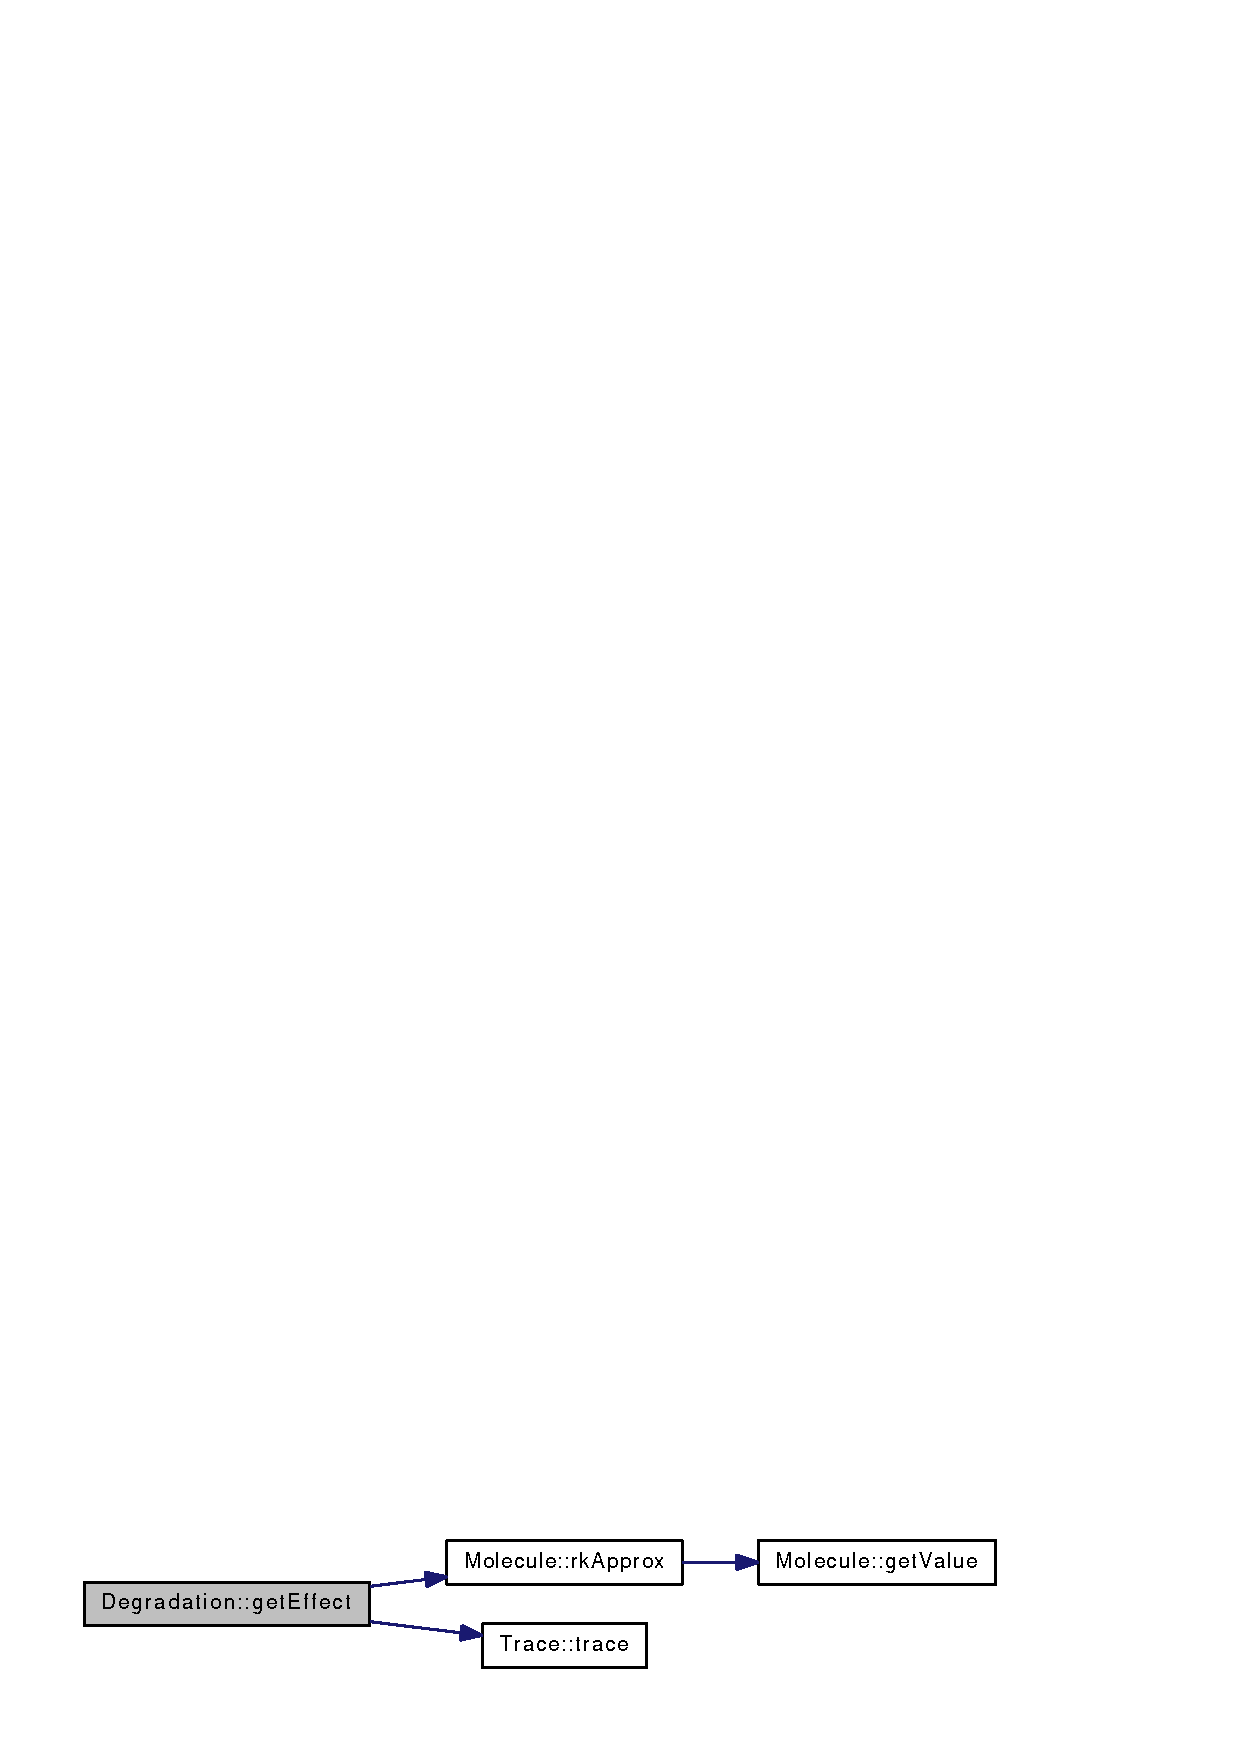
\includegraphics[width=241pt]{classDegradation_a3cad4fc84026c6f627306a7e35527f3c_cgraph}
\end{center}
\end{figure}


The documentation for this class was generated from the following files:\begin{DoxyCompactItemize}
\item 
\hyperlink{CustomInteractions_8h}{CustomInteractions.h}\item 
\hyperlink{CustomInteractions_8cpp}{CustomInteractions.cpp}\end{DoxyCompactItemize}

\hypertarget{classDerivGraph}{
\section{DerivGraph Class Reference}
\label{classDerivGraph}\index{DerivGraph@{DerivGraph}}
}


{\ttfamily \#include $<$DerivGraph.h$>$}\subsection*{Public Member Functions}
\begin{DoxyCompactItemize}
\item 
\hyperlink{classDerivGraph_af2a1f80b96b4657e7575748942d09947}{DerivGraph} ()
\item 
\hyperlink{classDerivGraph_a27b4fed56f8d2a745582622b7cb78b50}{$\sim$DerivGraph} ()
\item 
void \hyperlink{classDerivGraph_abf589f6aabe2c66bbe6f1aeb68ff4593}{test} ()
\item 
void \hyperlink{classDerivGraph_aa0921b8a7407be67085e9a11750a7263}{rungeKuttaEvaluate} (float, float)
\item 
void \hyperlink{classDerivGraph_a2e2ed79e21c6896a859cc7800d950809}{outputDotImage} (int, int)
\item 
void \hyperlink{classDerivGraph_ae435e564c1fa8370453c952b1ea5e9ab}{outputDataPlot} (int, int, float)
\item 
\hyperlink{classMolecule}{Molecule} $\ast$ \hyperlink{classDerivGraph_aaaa9598e55cbd8c55585a0488e940516}{getBestMolecule} (int)
\item 
void \hyperlink{classDerivGraph_a9bec1192a5ffc41a3ef4527caa9cdb8f}{setLimits} (int, int, int, int)
\item 
void \hyperlink{classDerivGraph_a79249de71c4c870277abed71d484e2d5}{setKineticRateLimits} (float, float)
\item 
void \hyperlink{classDerivGraph_a03b18e0508b383e7e6b3b57fc9fa6e90}{setRungeKuttaEval} (float, float)
\item 
void \hyperlink{classDerivGraph_ab0a014cac7227943fe67f85f52d4e613}{setDefaultInitialConc} (float)
\item 
ListDigraph $\ast$ \hyperlink{classDerivGraph_ae657edb3b0bf358f75f498a2d56e0456}{getListDigraph} ()
\item 
ListDigraph::NodeMap$<$ \hyperlink{classMolecule}{Molecule} $\ast$ $>$ $\ast$ \hyperlink{classDerivGraph_a41cea20de6fd631deeb82f036bc823f4}{getNodeMap} ()
\item 
ListDigraph::ArcMap$<$ \hyperlink{classInteraction}{Interaction} $\ast$ $>$ $\ast$ \hyperlink{classDerivGraph_a5ff2dac34f1cdcc4b4abfc26f13da1ab}{getArcMap} ()
\item 
void \hyperlink{classDerivGraph_a8862d4f9ebbd3eced9d56a81fe91c4fb}{newBasic} ()
\item 
void \hyperlink{classDerivGraph_afbda567a3f51d05fad37eb46fc121a89}{forwardRateChange} ()
\item 
void \hyperlink{classDerivGraph_aae8c58e1d6be852efbe1ed6593f31eca}{reverseRateChange} ()
\item 
void \hyperlink{classDerivGraph_a038841806aa1fe80a9450f977baa1fd2}{degradationRateChange} ()
\item 
\hyperlink{classDNA}{DNA} $\ast$ \hyperlink{classDerivGraph_ae39d9acba4901f668d8a85c88bfcc21a}{histoneMod} ()
\item 
void \hyperlink{classDerivGraph_a4be722e989002430ca7c363dce500638}{newComplex} ()
\item 
void \hyperlink{classDerivGraph_aa55a36103c33d4f1bd57de797bcd45cb}{newPromoter} ()
\item 
void \hyperlink{classDerivGraph_a83937a5c3ed427ebaad2bf23260c0352}{newPTM} ()
\end{DoxyCompactItemize}
\subsection*{Public Attributes}
\begin{DoxyCompactItemize}
\item 
MTRand \hyperlink{classDerivGraph_a2d5931b4ca8a9c6e0c013a74a5cfbc7c}{r}
\end{DoxyCompactItemize}


\subsection{Constructor \& Destructor Documentation}
\hypertarget{classDerivGraph_af2a1f80b96b4657e7575748942d09947}{
\index{DerivGraph@{DerivGraph}!DerivGraph@{DerivGraph}}
\index{DerivGraph@{DerivGraph}!DerivGraph@{DerivGraph}}
\subsubsection[{DerivGraph}]{\setlength{\rightskip}{0pt plus 5cm}DerivGraph::DerivGraph ()}}
\label{classDerivGraph_af2a1f80b96b4657e7575748942d09947}
\hyperlink{classDerivGraph_af2a1f80b96b4657e7575748942d09947}{DerivGraph::DerivGraph()}

\hyperlink{classDerivGraph}{DerivGraph} constructor.

The \hyperlink{classDerivGraph}{DerivGraph} holds LEMON objects such as ListDigraph, NodeMap, and ArcMap. It also holds the data produced by Runge-\/Kutta and facilitates plotting using Gnuplot.

The derivatives describing the concentration of molecules in the cell can be represented as a directed graph.

Each Node represents a type of molecule in the cell, and each Arc represents an interaction which has an effect on the Nodes which it connects.

Allocates: 1 ListDigraph() object 1 ListDigraph::NodeMap objects 1 ListDigraph::ArcMap object 

Here is the call graph for this function:\nopagebreak
\begin{figure}[H]
\begin{center}
\leavevmode
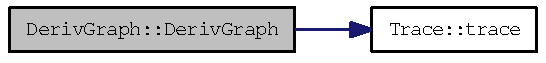
\includegraphics[width=149pt]{classDerivGraph_af2a1f80b96b4657e7575748942d09947_cgraph}
\end{center}
\end{figure}
\hypertarget{classDerivGraph_a27b4fed56f8d2a745582622b7cb78b50}{
\index{DerivGraph@{DerivGraph}!$\sim$DerivGraph@{$\sim$DerivGraph}}
\index{$\sim$DerivGraph@{$\sim$DerivGraph}!DerivGraph@{DerivGraph}}
\subsubsection[{$\sim$DerivGraph}]{\setlength{\rightskip}{0pt plus 5cm}DerivGraph::$\sim$DerivGraph ()}}
\label{classDerivGraph_a27b4fed56f8d2a745582622b7cb78b50}
\hyperlink{classDerivGraph_a27b4fed56f8d2a745582622b7cb78b50}{DerivGraph::$\sim$DerivGraph()}

\hyperlink{classDerivGraph}{DerivGraph} Destructor.

Frees: 1 NodeMap object n contained \hyperlink{classMolecule}{Molecule} objects 1 ArcMap object m contained \hyperlink{classInteraction}{Interaction} objects 1 ListDigraph object 

Here is the call graph for this function:\nopagebreak
\begin{figure}[H]
\begin{center}
\leavevmode
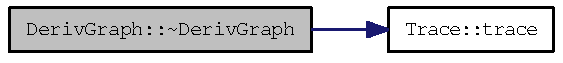
\includegraphics[width=153pt]{classDerivGraph_a27b4fed56f8d2a745582622b7cb78b50_cgraph}
\end{center}
\end{figure}


\subsection{Member Function Documentation}
\hypertarget{classDerivGraph_a038841806aa1fe80a9450f977baa1fd2}{
\index{DerivGraph@{DerivGraph}!degradationRateChange@{degradationRateChange}}
\index{degradationRateChange@{degradationRateChange}!DerivGraph@{DerivGraph}}
\subsubsection[{degradationRateChange}]{\setlength{\rightskip}{0pt plus 5cm}void DerivGraph::degradationRateChange ()}}
\label{classDerivGraph_a038841806aa1fe80a9450f977baa1fd2}
void \hyperlink{classDerivGraph_a038841806aa1fe80a9450f977baa1fd2}{DerivGraph::degradationRateChange()}

Randomly select a degradation interaction and modify its rate.

\hyperlink{classDegradation}{Degradation} interactions are of type \hyperlink{classDegradation}{Degradation} 

Here is the call graph for this function:\nopagebreak
\begin{figure}[H]
\begin{center}
\leavevmode
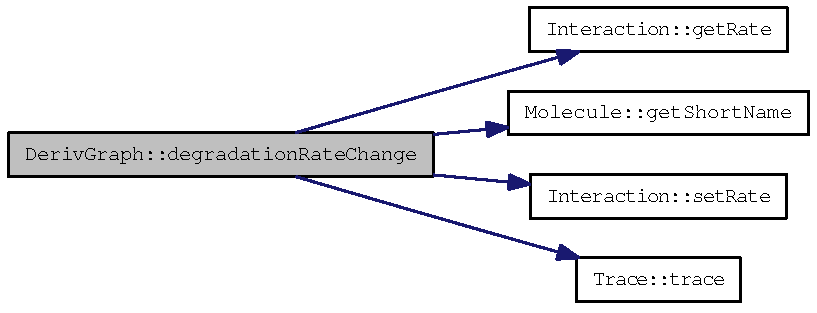
\includegraphics[width=214pt]{classDerivGraph_a038841806aa1fe80a9450f977baa1fd2_cgraph}
\end{center}
\end{figure}
\hypertarget{classDerivGraph_afbda567a3f51d05fad37eb46fc121a89}{
\index{DerivGraph@{DerivGraph}!forwardRateChange@{forwardRateChange}}
\index{forwardRateChange@{forwardRateChange}!DerivGraph@{DerivGraph}}
\subsubsection[{forwardRateChange}]{\setlength{\rightskip}{0pt plus 5cm}void DerivGraph::forwardRateChange ()}}
\label{classDerivGraph_afbda567a3f51d05fad37eb46fc121a89}
void \hyperlink{classDerivGraph_afbda567a3f51d05fad37eb46fc121a89}{DerivGraph::forwardRateChange()}

Randomly select a forward interaction and modify its rate.

Forward interactions are of type \hyperlink{classTranslation}{Translation}, ForwardComplex

TODO: add ForwardPTMs 

Here is the call graph for this function:\nopagebreak
\begin{figure}[H]
\begin{center}
\leavevmode
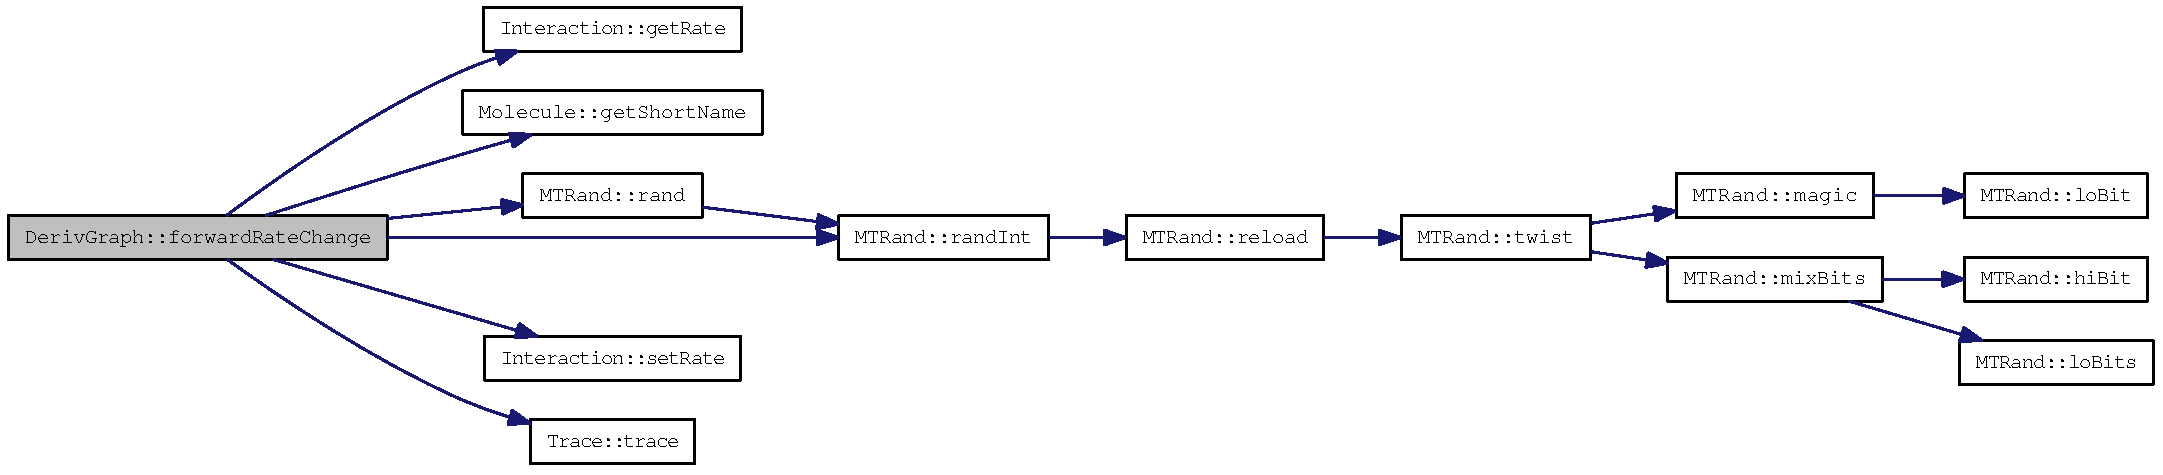
\includegraphics[width=203pt]{classDerivGraph_afbda567a3f51d05fad37eb46fc121a89_cgraph}
\end{center}
\end{figure}
\hypertarget{classDerivGraph_a5ff2dac34f1cdcc4b4abfc26f13da1ab}{
\index{DerivGraph@{DerivGraph}!getArcMap@{getArcMap}}
\index{getArcMap@{getArcMap}!DerivGraph@{DerivGraph}}
\subsubsection[{getArcMap}]{\setlength{\rightskip}{0pt plus 5cm}ListDigraph::ArcMap$<${\bf Interaction}$\ast$$>$$\ast$ DerivGraph::getArcMap ()}}
\label{classDerivGraph_a5ff2dac34f1cdcc4b4abfc26f13da1ab}
\hypertarget{classDerivGraph_aaaa9598e55cbd8c55585a0488e940516}{
\index{DerivGraph@{DerivGraph}!getBestMolecule@{getBestMolecule}}
\index{getBestMolecule@{getBestMolecule}!DerivGraph@{DerivGraph}}
\subsubsection[{getBestMolecule}]{\setlength{\rightskip}{0pt plus 5cm}{\bf Molecule} $\ast$ DerivGraph::getBestMolecule (int {\em CellID})}}
\label{classDerivGraph_aaaa9598e55cbd8c55585a0488e940516}


Here is the call graph for this function:\nopagebreak
\begin{figure}[H]
\begin{center}
\leavevmode
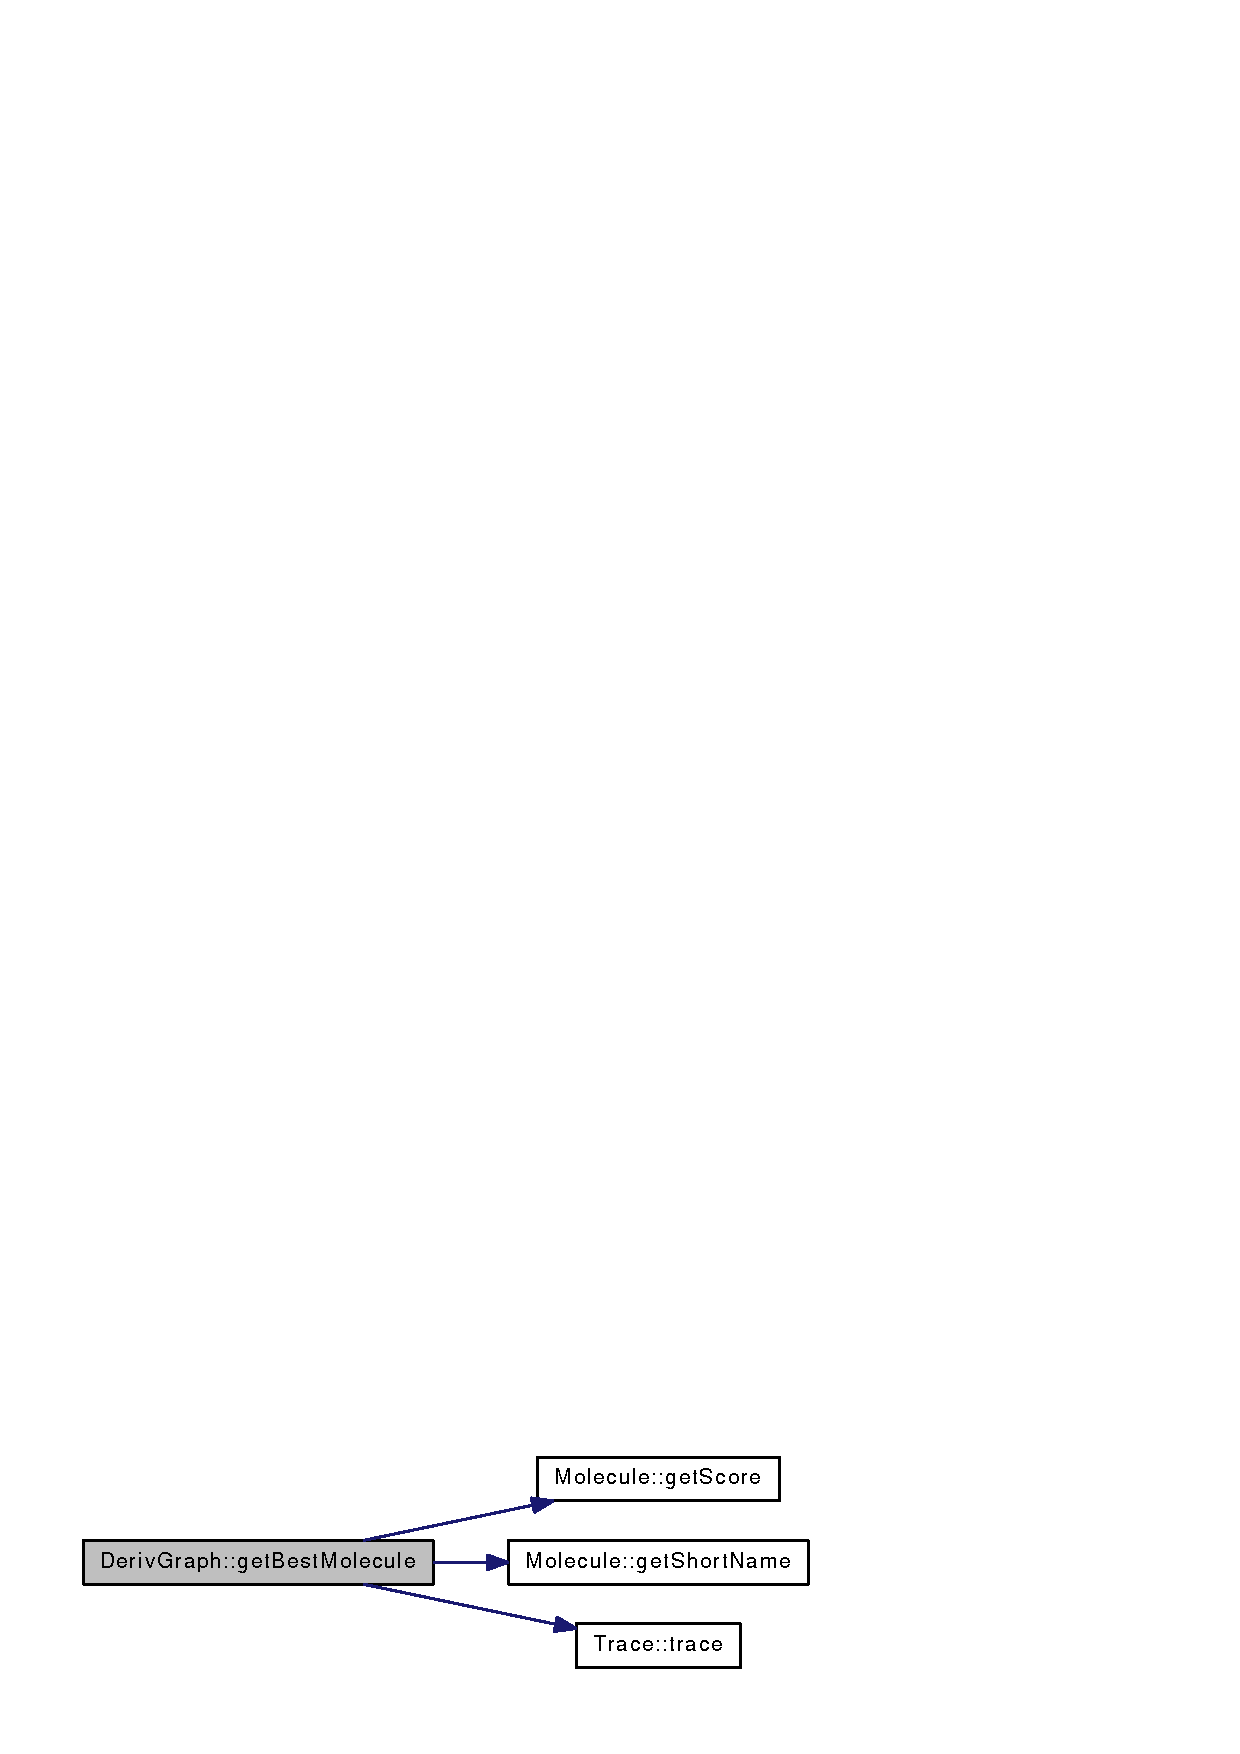
\includegraphics[width=215pt]{classDerivGraph_aaaa9598e55cbd8c55585a0488e940516_cgraph}
\end{center}
\end{figure}
\hypertarget{classDerivGraph_ae657edb3b0bf358f75f498a2d56e0456}{
\index{DerivGraph@{DerivGraph}!getListDigraph@{getListDigraph}}
\index{getListDigraph@{getListDigraph}!DerivGraph@{DerivGraph}}
\subsubsection[{getListDigraph}]{\setlength{\rightskip}{0pt plus 5cm}ListDigraph$\ast$ DerivGraph::getListDigraph ()}}
\label{classDerivGraph_ae657edb3b0bf358f75f498a2d56e0456}
\hypertarget{classDerivGraph_a41cea20de6fd631deeb82f036bc823f4}{
\index{DerivGraph@{DerivGraph}!getNodeMap@{getNodeMap}}
\index{getNodeMap@{getNodeMap}!DerivGraph@{DerivGraph}}
\subsubsection[{getNodeMap}]{\setlength{\rightskip}{0pt plus 5cm}ListDigraph::NodeMap$<${\bf Molecule}$\ast$$>$$\ast$ DerivGraph::getNodeMap ()}}
\label{classDerivGraph_a41cea20de6fd631deeb82f036bc823f4}
\hypertarget{classDerivGraph_ae39d9acba4901f668d8a85c88bfcc21a}{
\index{DerivGraph@{DerivGraph}!histoneMod@{histoneMod}}
\index{histoneMod@{histoneMod}!DerivGraph@{DerivGraph}}
\subsubsection[{histoneMod}]{\setlength{\rightskip}{0pt plus 5cm}{\bf DNA} $\ast$ DerivGraph::histoneMod ()}}
\label{classDerivGraph_ae39d9acba4901f668d8a85c88bfcc21a}
void \hyperlink{classDerivGraph_ae39d9acba4901f668d8a85c88bfcc21a}{DerivGraph::histoneMod()}

Randomly select a \hyperlink{classDNA}{DNA} molecule, and set the Histone factor to a random value \mbox{[}0,2\mbox{]}.

The histone value is a constant multiplied factor applied to the rate of \hyperlink{classmRNA}{mRNA} production by a \hyperlink{classDNA}{DNA} molecule. It is initialized at 1.0, and is randomly assigned a value between \mbox{[}0,2\mbox{]}.

A value \mbox{[}0,1) results in repression of \hyperlink{classmRNA}{mRNA} production. A value (1,2\mbox{]} results in activation of \hyperlink{classmRNA}{mRNA} production. 

Here is the call graph for this function:\nopagebreak
\begin{figure}[H]
\begin{center}
\leavevmode
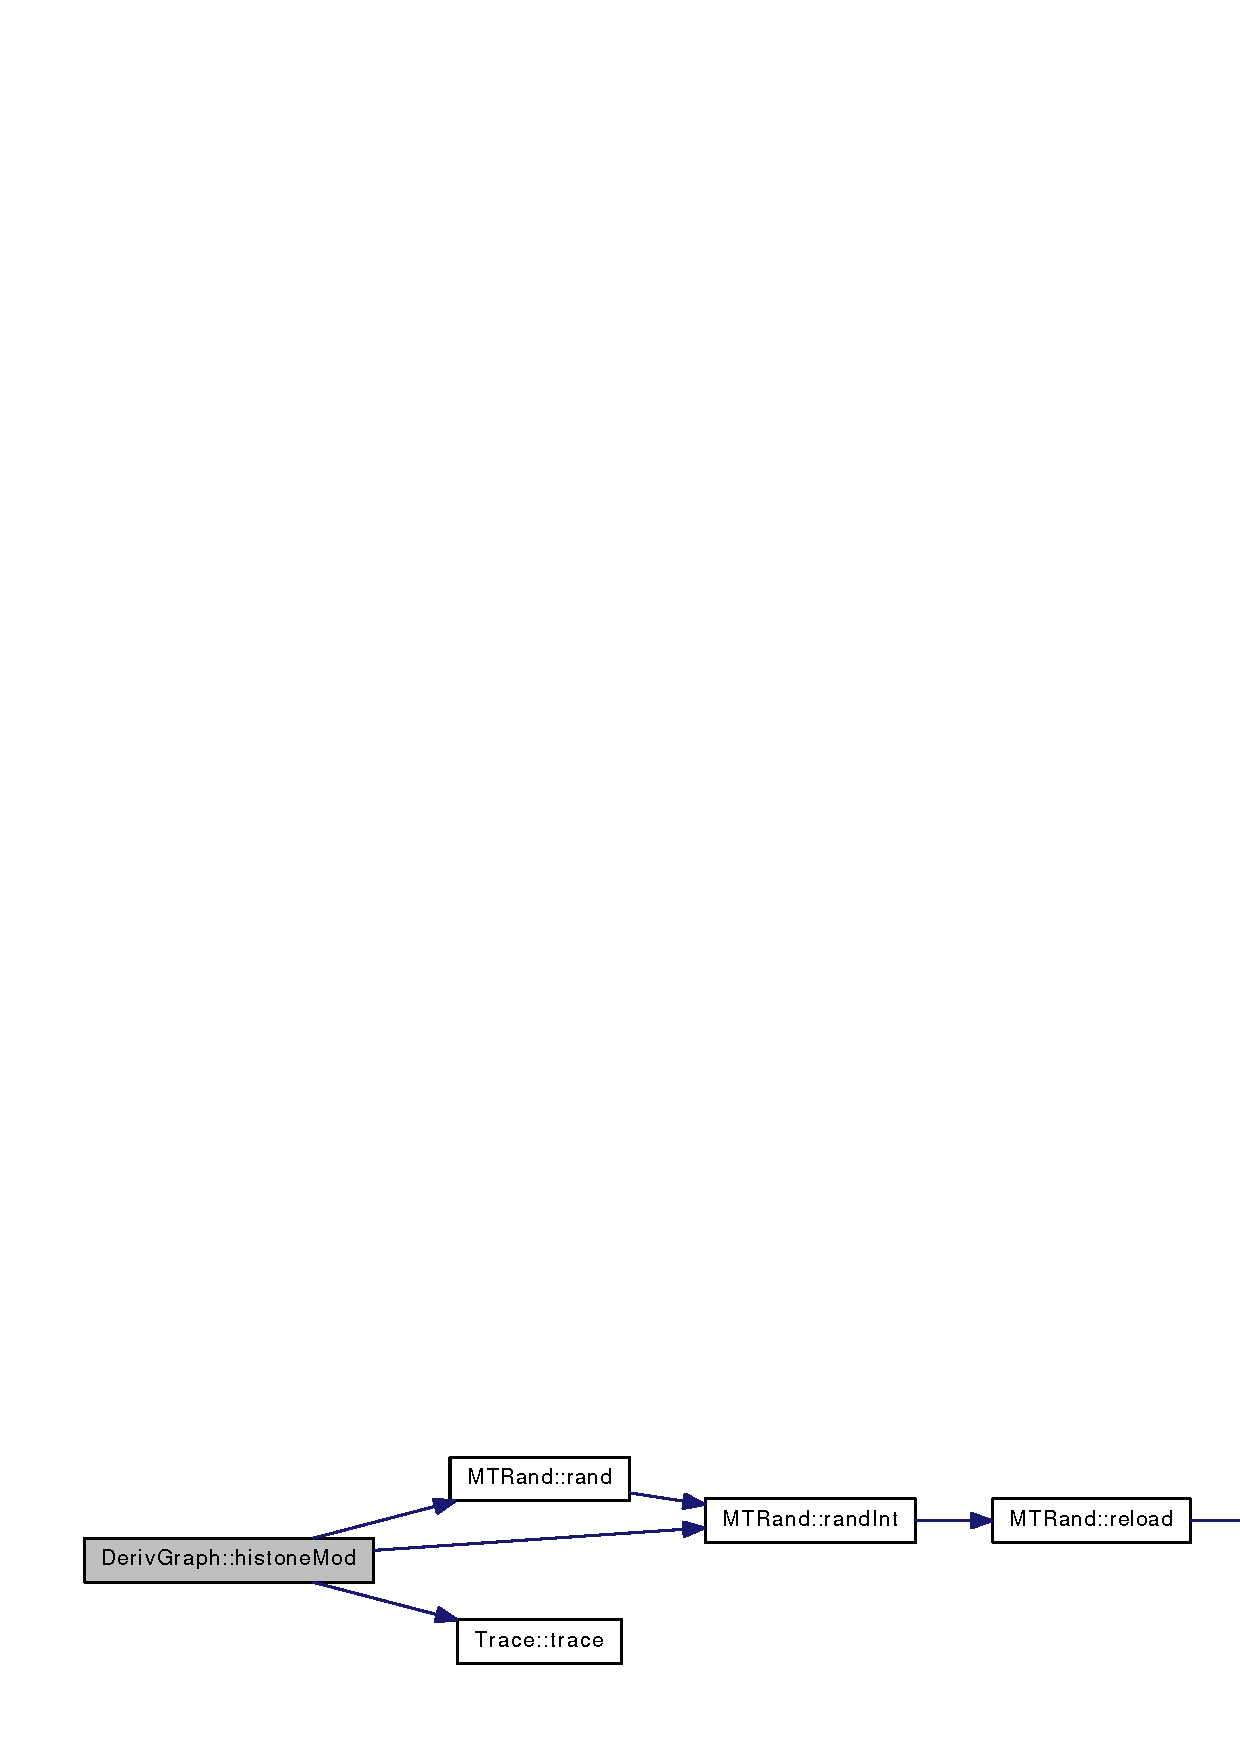
\includegraphics[width=150pt]{classDerivGraph_ae39d9acba4901f668d8a85c88bfcc21a_cgraph}
\end{center}
\end{figure}
\hypertarget{classDerivGraph_a8862d4f9ebbd3eced9d56a81fe91c4fb}{
\index{DerivGraph@{DerivGraph}!newBasic@{newBasic}}
\index{newBasic@{newBasic}!DerivGraph@{DerivGraph}}
\subsubsection[{newBasic}]{\setlength{\rightskip}{0pt plus 5cm}void DerivGraph::newBasic ()}}
\label{classDerivGraph_a8862d4f9ebbd3eced9d56a81fe91c4fb}
\hyperlink{classDerivGraph_a8862d4f9ebbd3eced9d56a81fe91c4fb}{DerivGraph::newBasic()}

Create a new \hyperlink{classDNA}{DNA}, \hyperlink{classmRNA}{mRNA}, and protein in the cell.

\hyperlink{classDNA}{DNA} -\/-\/-\/$>$ \hyperlink{classmRNA}{mRNA} -\/-\/-\/-\/$>$ \hyperlink{classProtein}{Protein} $|$ $|$ v v Deg Deg 

Here is the call graph for this function:\nopagebreak
\begin{figure}[H]
\begin{center}
\leavevmode
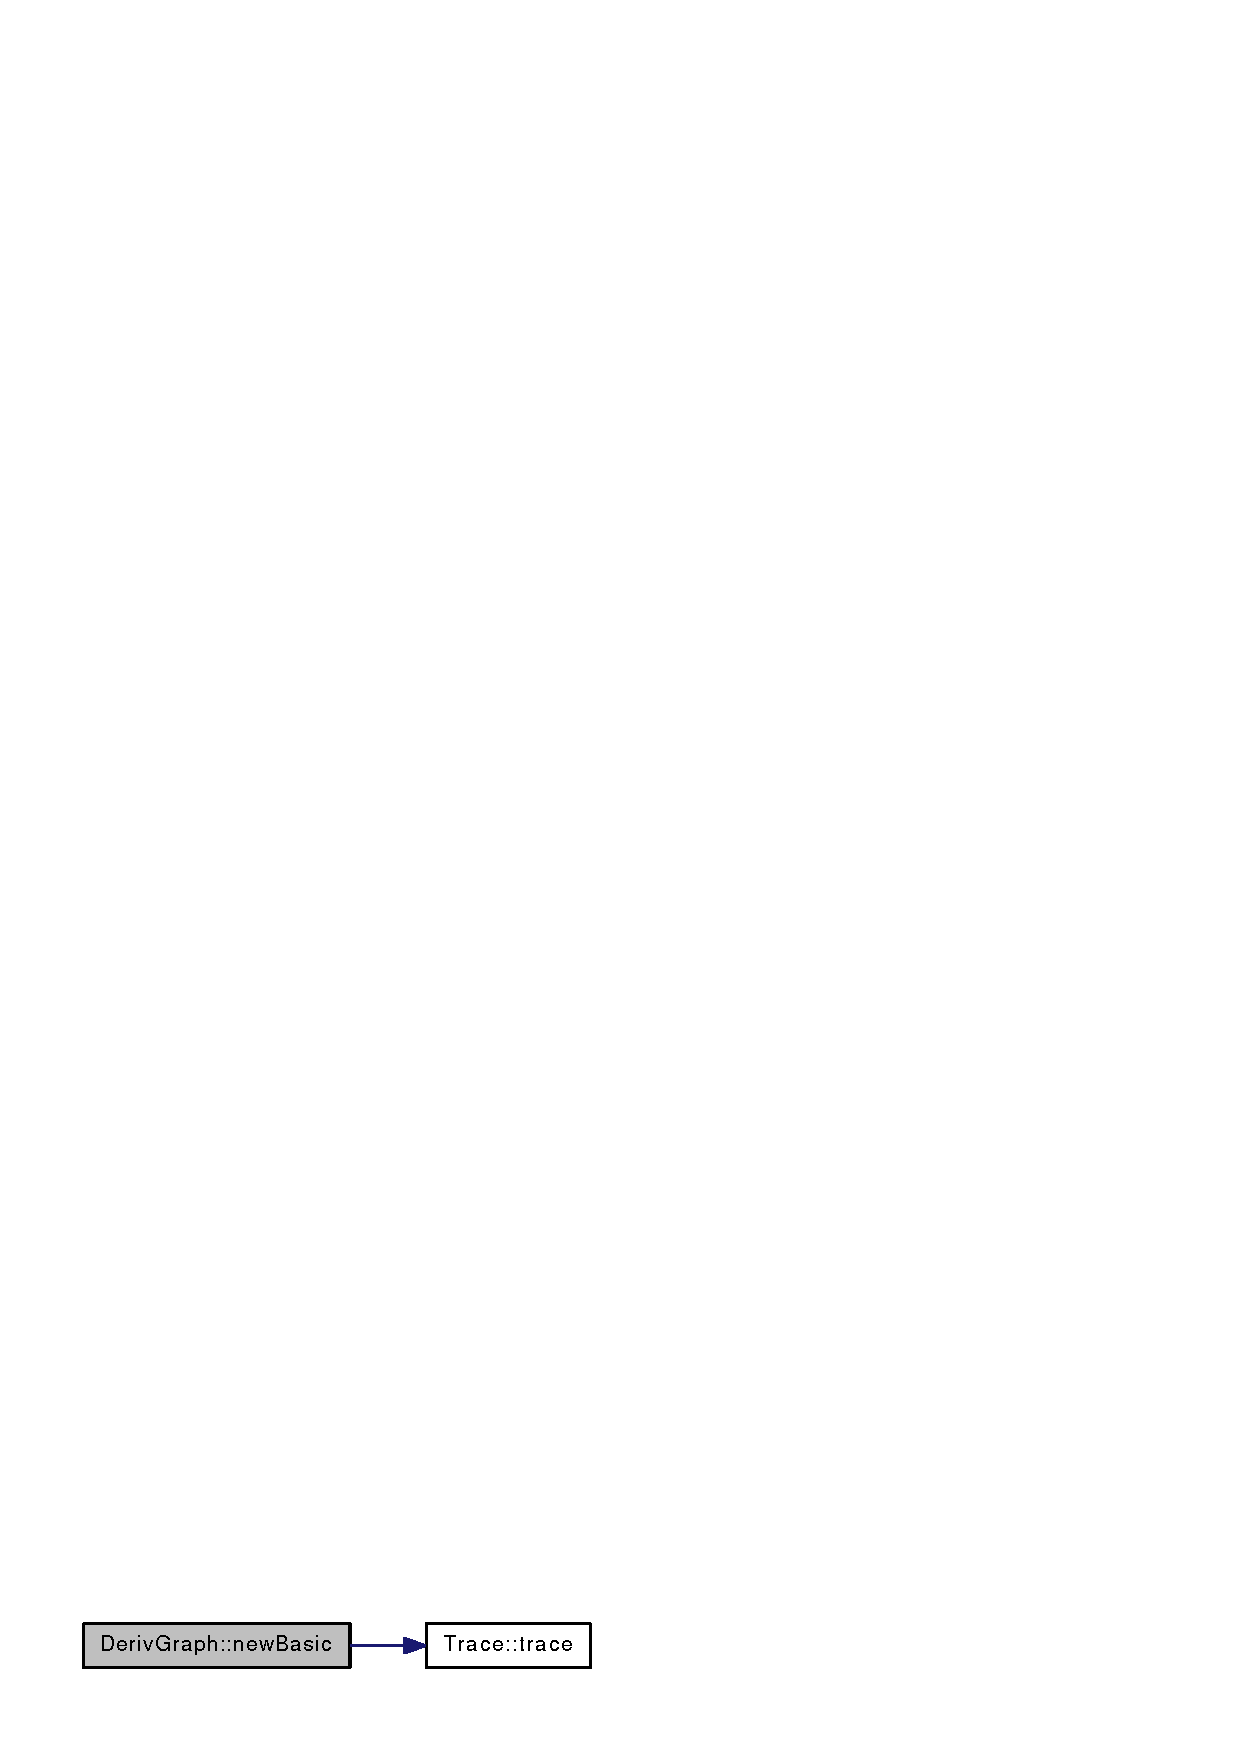
\includegraphics[width=144pt]{classDerivGraph_a8862d4f9ebbd3eced9d56a81fe91c4fb_cgraph}
\end{center}
\end{figure}
\hypertarget{classDerivGraph_a4be722e989002430ca7c363dce500638}{
\index{DerivGraph@{DerivGraph}!newComplex@{newComplex}}
\index{newComplex@{newComplex}!DerivGraph@{DerivGraph}}
\subsubsection[{newComplex}]{\setlength{\rightskip}{0pt plus 5cm}void DerivGraph::newComplex ()}}
\label{classDerivGraph_a4be722e989002430ca7c363dce500638}
void \hyperlink{classDerivGraph_a4be722e989002430ca7c363dce500638}{DerivGraph::newComplex()}

Randomly select two \hyperlink{classProtein}{Protein} molecules to be complexed together.

If the two selected proteins already exist in a complex reaction together, the mutation will fail.

Molecules which can complex together are \hyperlink{classProtein}{Protein}, and ComplexProteins

TODO: add PTM's to the possible complex 

Here is the call graph for this function:\nopagebreak
\begin{figure}[H]
\begin{center}
\leavevmode
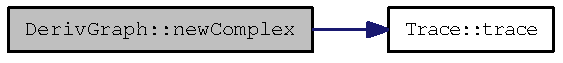
\includegraphics[width=153pt]{classDerivGraph_a4be722e989002430ca7c363dce500638_cgraph}
\end{center}
\end{figure}
\hypertarget{classDerivGraph_aa55a36103c33d4f1bd57de797bcd45cb}{
\index{DerivGraph@{DerivGraph}!newPromoter@{newPromoter}}
\index{newPromoter@{newPromoter}!DerivGraph@{DerivGraph}}
\subsubsection[{newPromoter}]{\setlength{\rightskip}{0pt plus 5cm}void DerivGraph::newPromoter ()}}
\label{classDerivGraph_aa55a36103c33d4f1bd57de797bcd45cb}
void \hyperlink{classDerivGraph_aa55a36103c33d4f1bd57de797bcd45cb}{DerivGraph::newPromoter()}

Select a random protein and \hyperlink{classDNA}{DNA} to add a Protein-\/Promoter interaction to.

The Protein-\/Promoter interaction is used in conjunction with the Hill model of cooperativity, and affects the Goodwin term used by \hyperlink{classDNA}{DNA} to calculate the rate of production. 

Here is the call graph for this function:\nopagebreak
\begin{figure}[H]
\begin{center}
\leavevmode
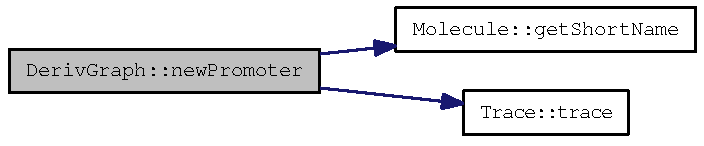
\includegraphics[width=187pt]{classDerivGraph_aa55a36103c33d4f1bd57de797bcd45cb_cgraph}
\end{center}
\end{figure}
\hypertarget{classDerivGraph_a83937a5c3ed427ebaad2bf23260c0352}{
\index{DerivGraph@{DerivGraph}!newPTM@{newPTM}}
\index{newPTM@{newPTM}!DerivGraph@{DerivGraph}}
\subsubsection[{newPTM}]{\setlength{\rightskip}{0pt plus 5cm}void DerivGraph::newPTM ()}}
\label{classDerivGraph_a83937a5c3ed427ebaad2bf23260c0352}
void \hyperlink{classDerivGraph_a83937a5c3ed427ebaad2bf23260c0352}{DerivGraph::newPTM()}

Randomly select a \hyperlink{classProtein}{Protein} molecule to which a PTM should be applied. The new PTM \hyperlink{classProtein}{Protein} has the same counts of modifications, with a random index incremented by one to reflect the new value. A PTM can be applied to a basic protein or a previously existing PTM.

TODO: check if a PTM already exists on a protein and prevent duplicate PTM's 

Here is the call graph for this function:\nopagebreak
\begin{figure}[H]
\begin{center}
\leavevmode
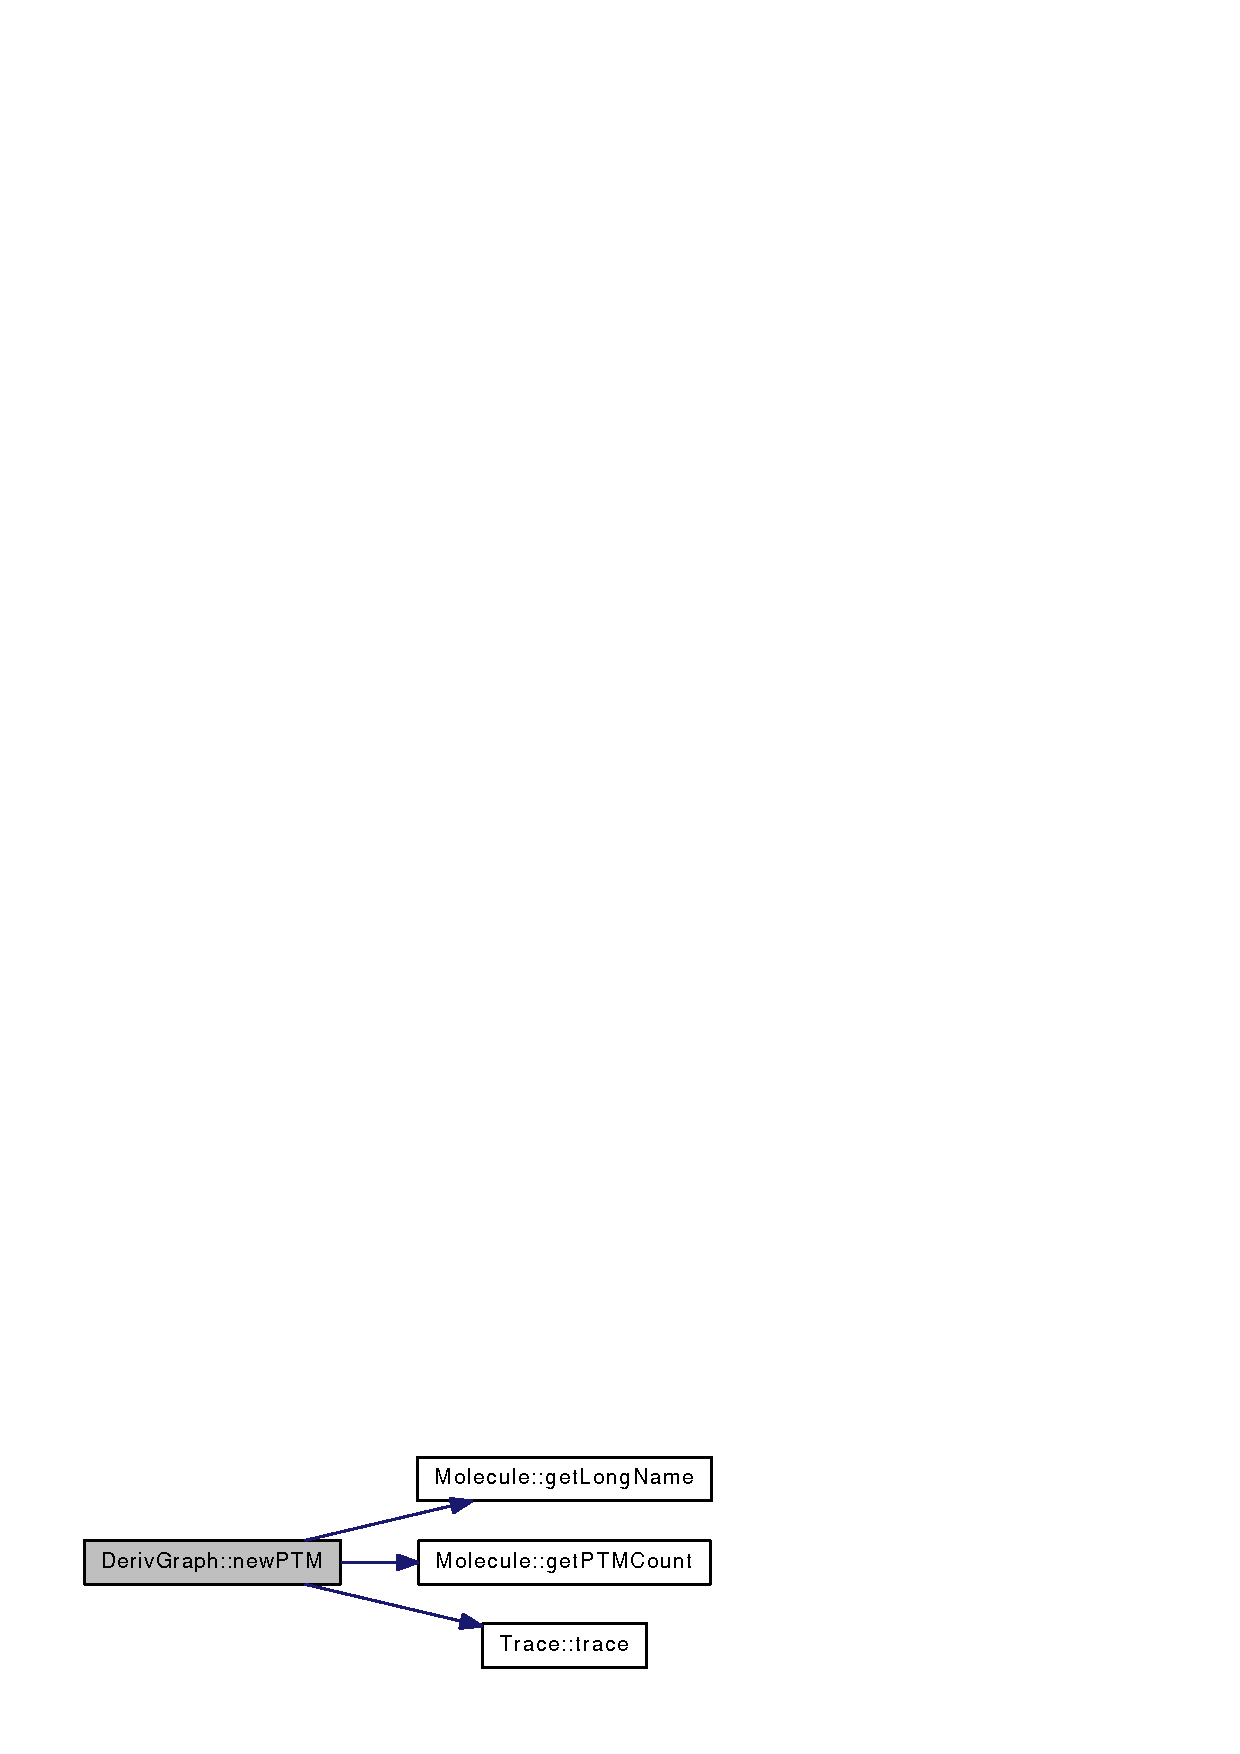
\includegraphics[width=173pt]{classDerivGraph_a83937a5c3ed427ebaad2bf23260c0352_cgraph}
\end{center}
\end{figure}
\hypertarget{classDerivGraph_ae435e564c1fa8370453c952b1ea5e9ab}{
\index{DerivGraph@{DerivGraph}!outputDataPlot@{outputDataPlot}}
\index{outputDataPlot@{outputDataPlot}!DerivGraph@{DerivGraph}}
\subsubsection[{outputDataPlot}]{\setlength{\rightskip}{0pt plus 5cm}void DerivGraph::outputDataPlot (int {\em cellNum}, \/  int {\em gen}, \/  float {\em step})}}
\label{classDerivGraph_ae435e564c1fa8370453c952b1ea5e9ab}
void \hyperlink{classDerivGraph_ae435e564c1fa8370453c952b1ea5e9ab}{DerivGraph::outputDataPlot(int, int, float)}

Output a png image of the concentration data of molecules plotted by Gnuplot.

For each molecule in the MoleculeList, a process running gnuplot is forked to which data from Runge-\/Kutta is fed to produce a plot.


\begin{DoxyParams}{Parameters}
\item[{\em cellNum}]the cell number to put in the filename \item[{\em gen}]the generation number to put in the filename \item[{\em step}]the stepSize used between the rungeKuttaSolution data points \end{DoxyParams}
\hypertarget{classDerivGraph_a2e2ed79e21c6896a859cc7800d950809}{
\index{DerivGraph@{DerivGraph}!outputDotImage@{outputDotImage}}
\index{outputDotImage@{outputDotImage}!DerivGraph@{DerivGraph}}
\subsubsection[{outputDotImage}]{\setlength{\rightskip}{0pt plus 5cm}void DerivGraph::outputDotImage (int {\em cellNum}, \/  int {\em gen})}}
\label{classDerivGraph_a2e2ed79e21c6896a859cc7800d950809}
void \hyperlink{classDerivGraph_a2e2ed79e21c6896a859cc7800d950809}{DerivGraph::outputDotImage(int, int)}

Output a png image of the current graph structure using GraphViz.

A process running GraphViz is forked and a pipe opened to its standard in. The general layout of the output file can be changed below. The Node and Arc names are defined within the \hyperlink{classMolecule}{Molecule} and \hyperlink{classInteraction}{Interaction} classes.


\begin{DoxyParams}{Parameters}
\item[{\em cellNum}]the cell number to put in the filename \item[{\em gen}]the generation number to put in the filename \end{DoxyParams}
\hypertarget{classDerivGraph_aae8c58e1d6be852efbe1ed6593f31eca}{
\index{DerivGraph@{DerivGraph}!reverseRateChange@{reverseRateChange}}
\index{reverseRateChange@{reverseRateChange}!DerivGraph@{DerivGraph}}
\subsubsection[{reverseRateChange}]{\setlength{\rightskip}{0pt plus 5cm}void DerivGraph::reverseRateChange ()}}
\label{classDerivGraph_aae8c58e1d6be852efbe1ed6593f31eca}
void \hyperlink{classDerivGraph_aae8c58e1d6be852efbe1ed6593f31eca}{DerivGraph::reverseRateChange()}

Randomly select a reverse interaction and modify its rate.

Reverse interactions are of type \hyperlink{classReverseComplexation}{ReverseComplexation}, \hyperlink{classReversePTM}{ReversePTM} 

Here is the call graph for this function:\nopagebreak
\begin{figure}[H]
\begin{center}
\leavevmode
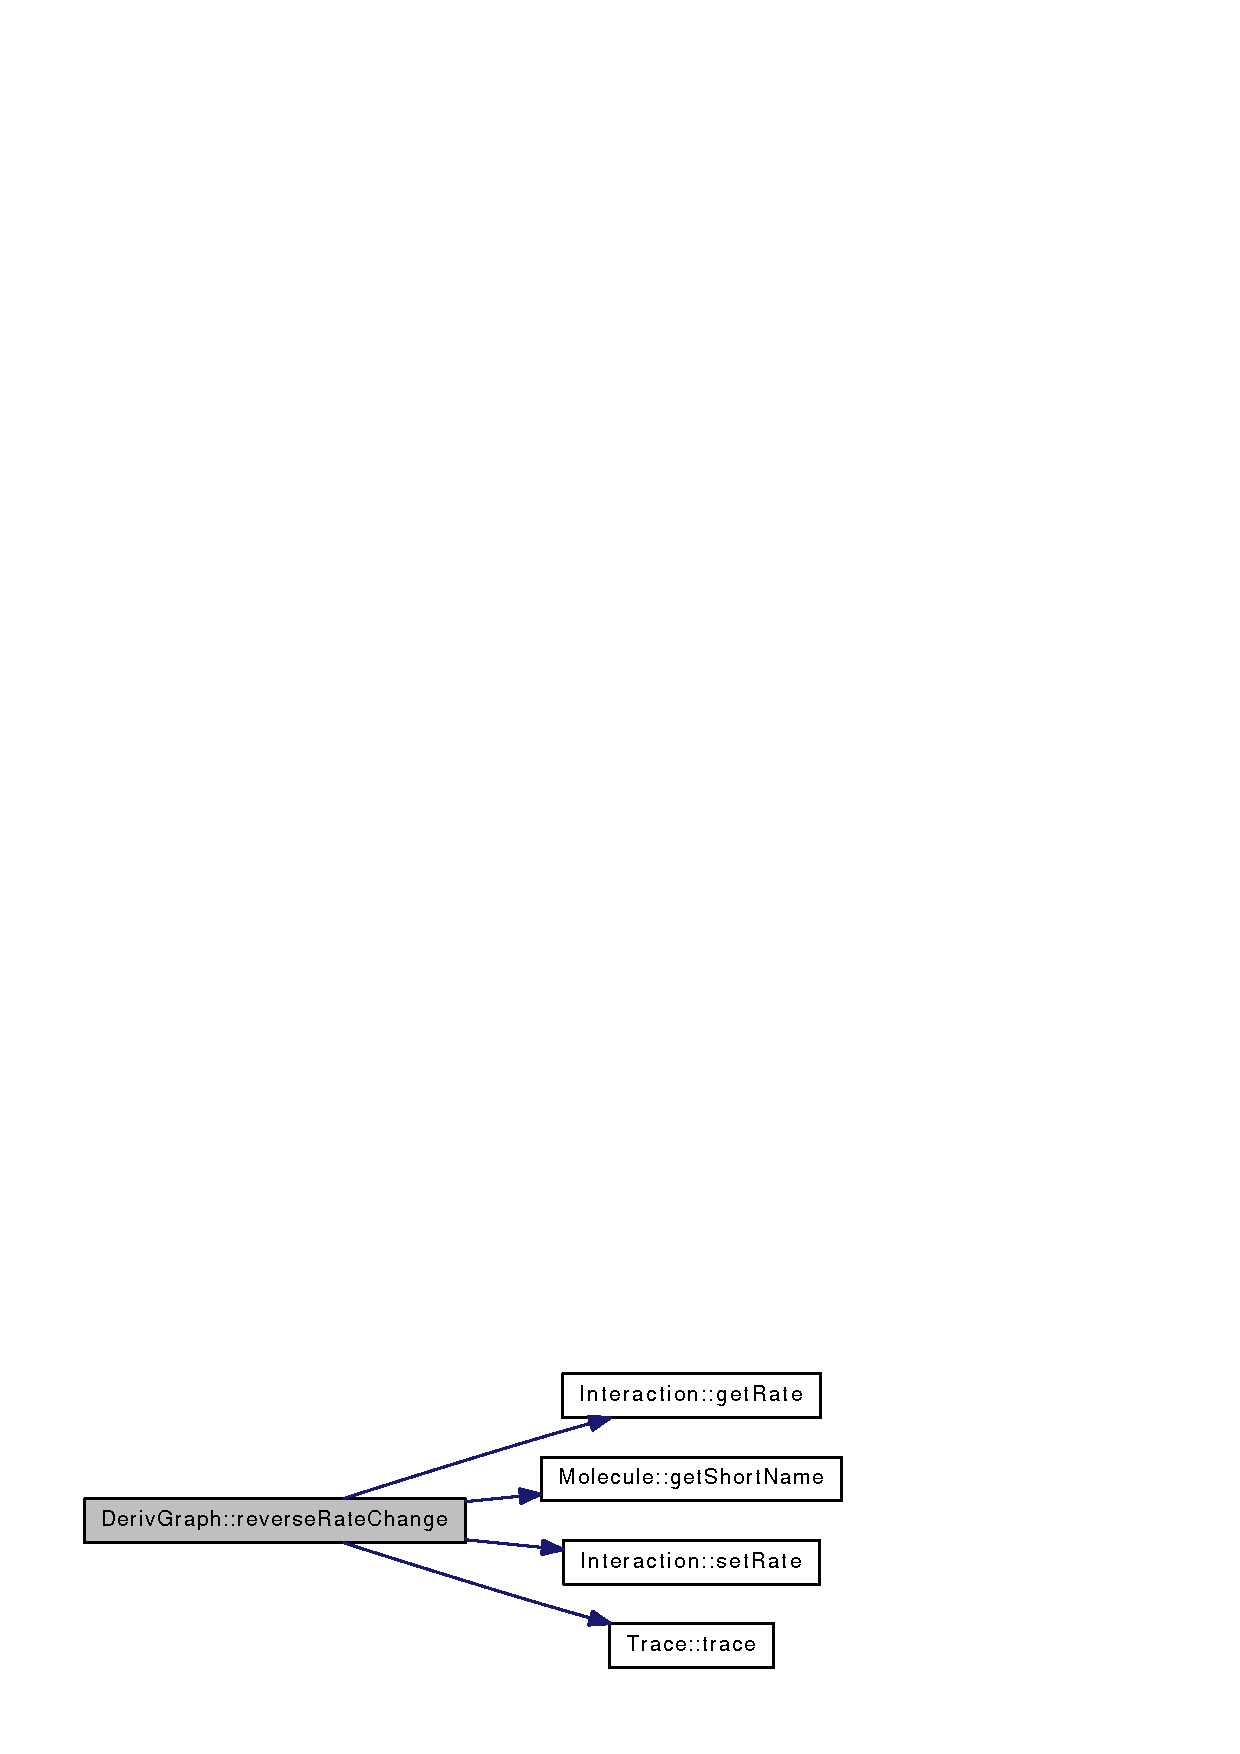
\includegraphics[width=204pt]{classDerivGraph_aae8c58e1d6be852efbe1ed6593f31eca_cgraph}
\end{center}
\end{figure}
\hypertarget{classDerivGraph_aa0921b8a7407be67085e9a11750a7263}{
\index{DerivGraph@{DerivGraph}!rungeKuttaEvaluate@{rungeKuttaEvaluate}}
\index{rungeKuttaEvaluate@{rungeKuttaEvaluate}!DerivGraph@{DerivGraph}}
\subsubsection[{rungeKuttaEvaluate}]{\setlength{\rightskip}{0pt plus 5cm}void DerivGraph::rungeKuttaEvaluate (float {\em rkStep}, \/  float {\em rkLimit})}}
\label{classDerivGraph_aa0921b8a7407be67085e9a11750a7263}
Uses the Runge-\/Kutta fourth order method to approximate the solutions to the system of differential equations

The result of this algorithm is the vector rungeKuttaSolution within each \hyperlink{classMolecule}{Molecule} object containing the approximation of the concentration at each timestep.


\begin{DoxyParams}{Parameters}
\item[{\em rkStep}]the timestep (precision) between calculated points \end{DoxyParams}
\hypertarget{classDerivGraph_ab0a014cac7227943fe67f85f52d4e613}{
\index{DerivGraph@{DerivGraph}!setDefaultInitialConc@{setDefaultInitialConc}}
\index{setDefaultInitialConc@{setDefaultInitialConc}!DerivGraph@{DerivGraph}}
\subsubsection[{setDefaultInitialConc}]{\setlength{\rightskip}{0pt plus 5cm}void DerivGraph::setDefaultInitialConc (float {\em initial\_\-conc})}}
\label{classDerivGraph_ab0a014cac7227943fe67f85f52d4e613}
DerivGraph::setDefaultInitialConcentration(float)

Set the default initial concentration for molecules


\begin{DoxyParams}{Parameters}
\item[{\em initial\_\-conc}]The initial concentration for new molecules \end{DoxyParams}
\hypertarget{classDerivGraph_a79249de71c4c870277abed71d484e2d5}{
\index{DerivGraph@{DerivGraph}!setKineticRateLimits@{setKineticRateLimits}}
\index{setKineticRateLimits@{setKineticRateLimits}!DerivGraph@{DerivGraph}}
\subsubsection[{setKineticRateLimits}]{\setlength{\rightskip}{0pt plus 5cm}void DerivGraph::setKineticRateLimits (float {\em min\_\-kinetic\_\-rate}, \/  float {\em max\_\-kinetic\_\-rate})}}
\label{classDerivGraph_a79249de71c4c870277abed71d484e2d5}
\hyperlink{classDerivGraph_a79249de71c4c870277abed71d484e2d5}{DerivGraph::setKineticRateLimits(float, float)}

Assign lower and upper bounds to the randomly generated kinetic rates


\begin{DoxyParams}{Parameters}
\item[{\em min\_\-kinetic\_\-rate}]The lower bound on random kinetic rates \item[{\em max\_\-kinetic\_\-rate}]The upper bound on random kinetic rates \end{DoxyParams}
\hypertarget{classDerivGraph_a9bec1192a5ffc41a3ef4527caa9cdb8f}{
\index{DerivGraph@{DerivGraph}!setLimits@{setLimits}}
\index{setLimits@{setLimits}!DerivGraph@{DerivGraph}}
\subsubsection[{setLimits}]{\setlength{\rightskip}{0pt plus 5cm}void DerivGraph::setLimits (int {\em max\_\-basic}, \/  int {\em max\_\-ptm}, \/  int {\em max\_\-comp}, \/  int {\em max\_\-promoter})}}
\label{classDerivGraph_a9bec1192a5ffc41a3ef4527caa9cdb8f}
\hyperlink{classDerivGraph_a9bec1192a5ffc41a3ef4527caa9cdb8f}{DerivGraph::setLimits(int, int, int, int)}

Set the occurrence limits for mutation types


\begin{DoxyParams}{Parameters}
\item[{\em max\_\-basic}]Maximum basic proteins allowed \item[{\em max\_\-ptm}]Maximum number of post translationally modified proteins allowed \item[{\em max\_\-comp}]Maximum number of complexed proteins allowed \item[{\em max\_\-promoter}]Maximum number of protein-\/promoter interactions allowed \end{DoxyParams}


Here is the call graph for this function:\nopagebreak
\begin{figure}[H]
\begin{center}
\leavevmode
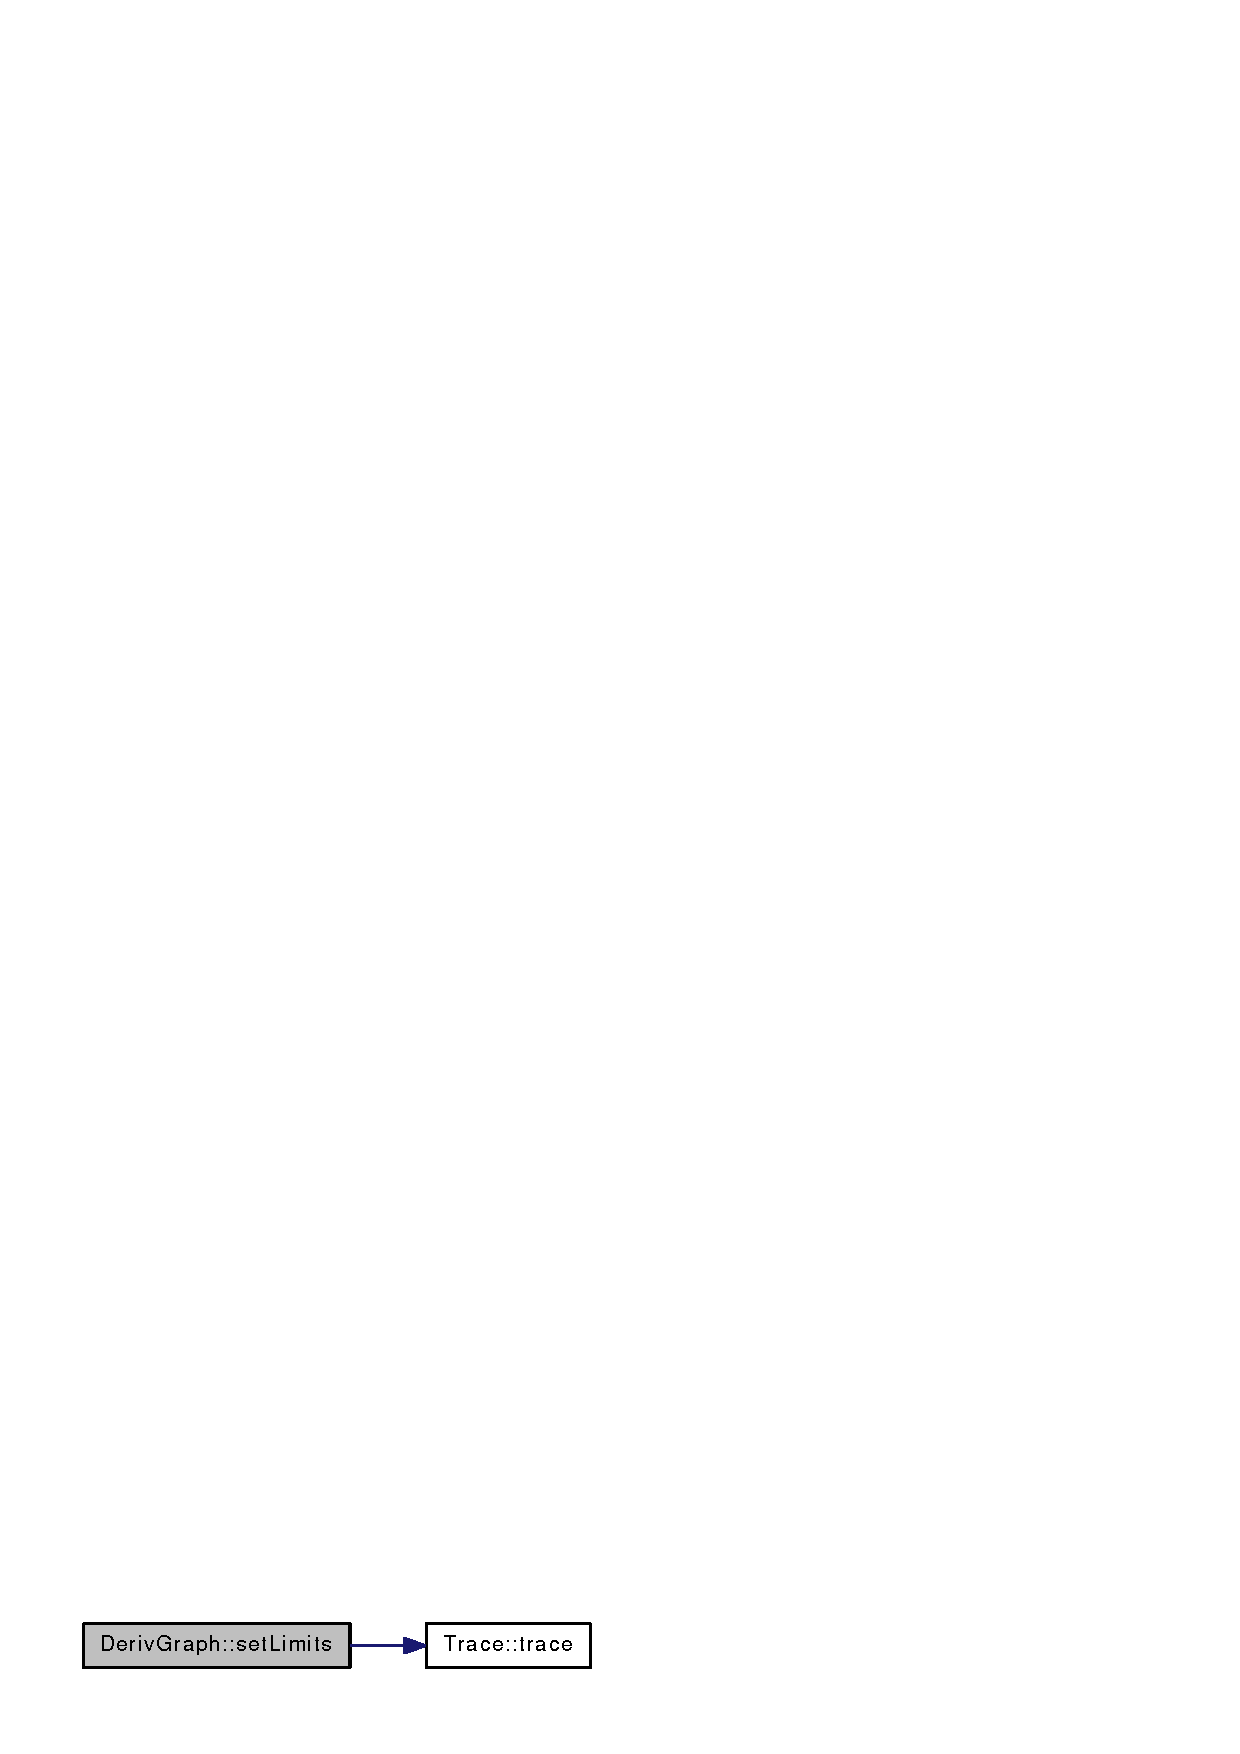
\includegraphics[width=144pt]{classDerivGraph_a9bec1192a5ffc41a3ef4527caa9cdb8f_cgraph}
\end{center}
\end{figure}
\hypertarget{classDerivGraph_a03b18e0508b383e7e6b3b57fc9fa6e90}{
\index{DerivGraph@{DerivGraph}!setRungeKuttaEval@{setRungeKuttaEval}}
\index{setRungeKuttaEval@{setRungeKuttaEval}!DerivGraph@{DerivGraph}}
\subsubsection[{setRungeKuttaEval}]{\setlength{\rightskip}{0pt plus 5cm}void DerivGraph::setRungeKuttaEval (float {\em rk\_\-time\_\-step}, \/  float {\em rk\_\-time\_\-limit})}}
\label{classDerivGraph_a03b18e0508b383e7e6b3b57fc9fa6e90}
\hyperlink{classDerivGraph_a03b18e0508b383e7e6b3b57fc9fa6e90}{DerivGraph::setRungeKuttaEval(float, float)}

Set the parameters for runge-\/kutta evalutation


\begin{DoxyParams}{Parameters}
\item[{\em rk\_\-time\_\-step}]The timestep between points (t, conc) calculated by Runge-\/Kutta \item[{\em rk\_\-time\_\-limit}]The upper time limit for Runge-\/Kutta calculation (time = x axis) \end{DoxyParams}
\hypertarget{classDerivGraph_abf589f6aabe2c66bbe6f1aeb68ff4593}{
\index{DerivGraph@{DerivGraph}!test@{test}}
\index{test@{test}!DerivGraph@{DerivGraph}}
\subsubsection[{test}]{\setlength{\rightskip}{0pt plus 5cm}void DerivGraph::test ()}}
\label{classDerivGraph_abf589f6aabe2c66bbe6f1aeb68ff4593}


Here is the call graph for this function:\nopagebreak
\begin{figure}[H]
\begin{center}
\leavevmode
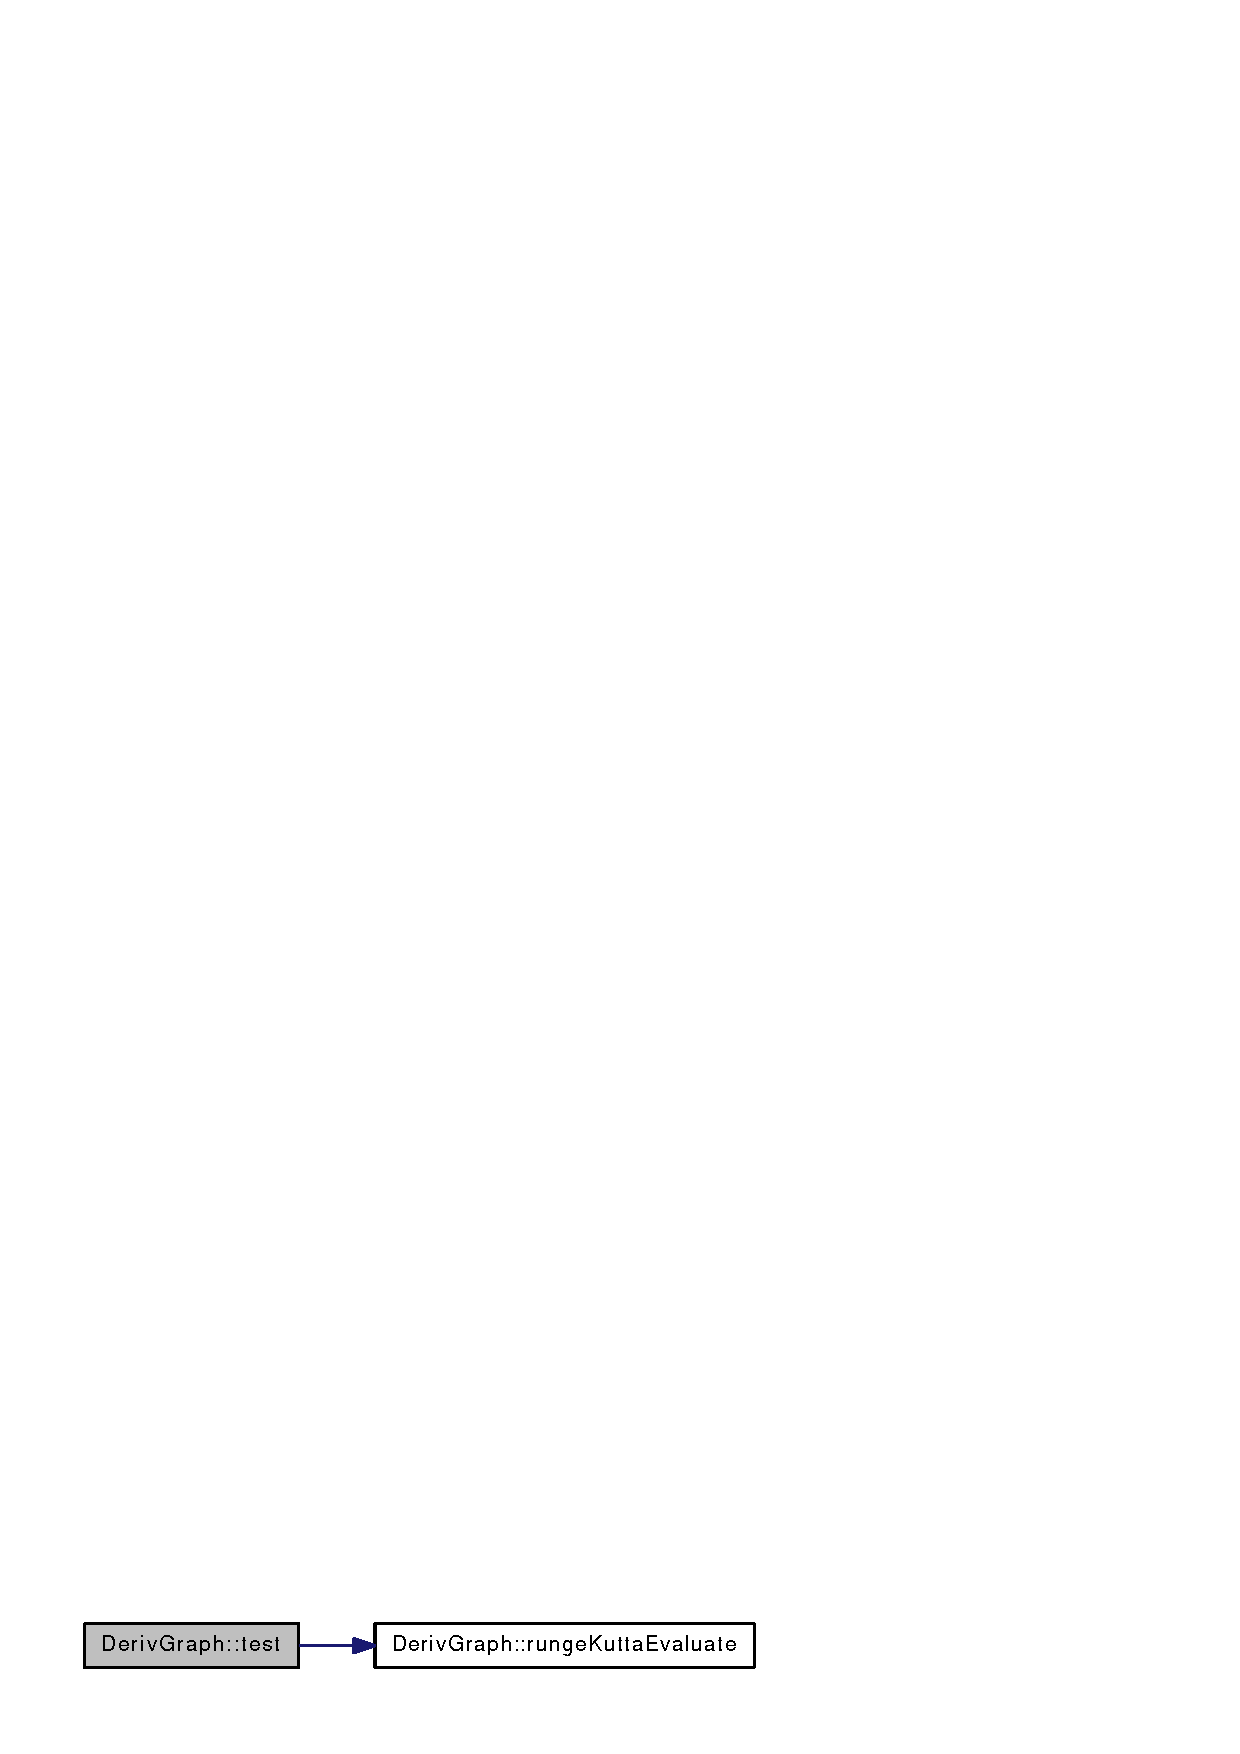
\includegraphics[width=183pt]{classDerivGraph_abf589f6aabe2c66bbe6f1aeb68ff4593_cgraph}
\end{center}
\end{figure}


\subsection{Member Data Documentation}
\hypertarget{classDerivGraph_a2d5931b4ca8a9c6e0c013a74a5cfbc7c}{
\index{DerivGraph@{DerivGraph}!r@{r}}
\index{r@{r}!DerivGraph@{DerivGraph}}
\subsubsection[{r}]{\setlength{\rightskip}{0pt plus 5cm}MTRand {\bf DerivGraph::r}}}
\label{classDerivGraph_a2d5931b4ca8a9c6e0c013a74a5cfbc7c}


The documentation for this class was generated from the following files:\begin{DoxyCompactItemize}
\item 
\hyperlink{DerivGraph_8h}{DerivGraph.h}\item 
\hyperlink{DerivGraph_8cpp}{DerivGraph.cpp}\end{DoxyCompactItemize}

\hypertarget{classDNA}{
\section{DNA Class Reference}
\label{classDNA}\index{DNA@{DNA}}
}


{\ttfamily \#include $<$CustomMolecules.h$>$}Inheritance diagram for DNA:\nopagebreak
\begin{figure}[H]
\begin{center}
\leavevmode
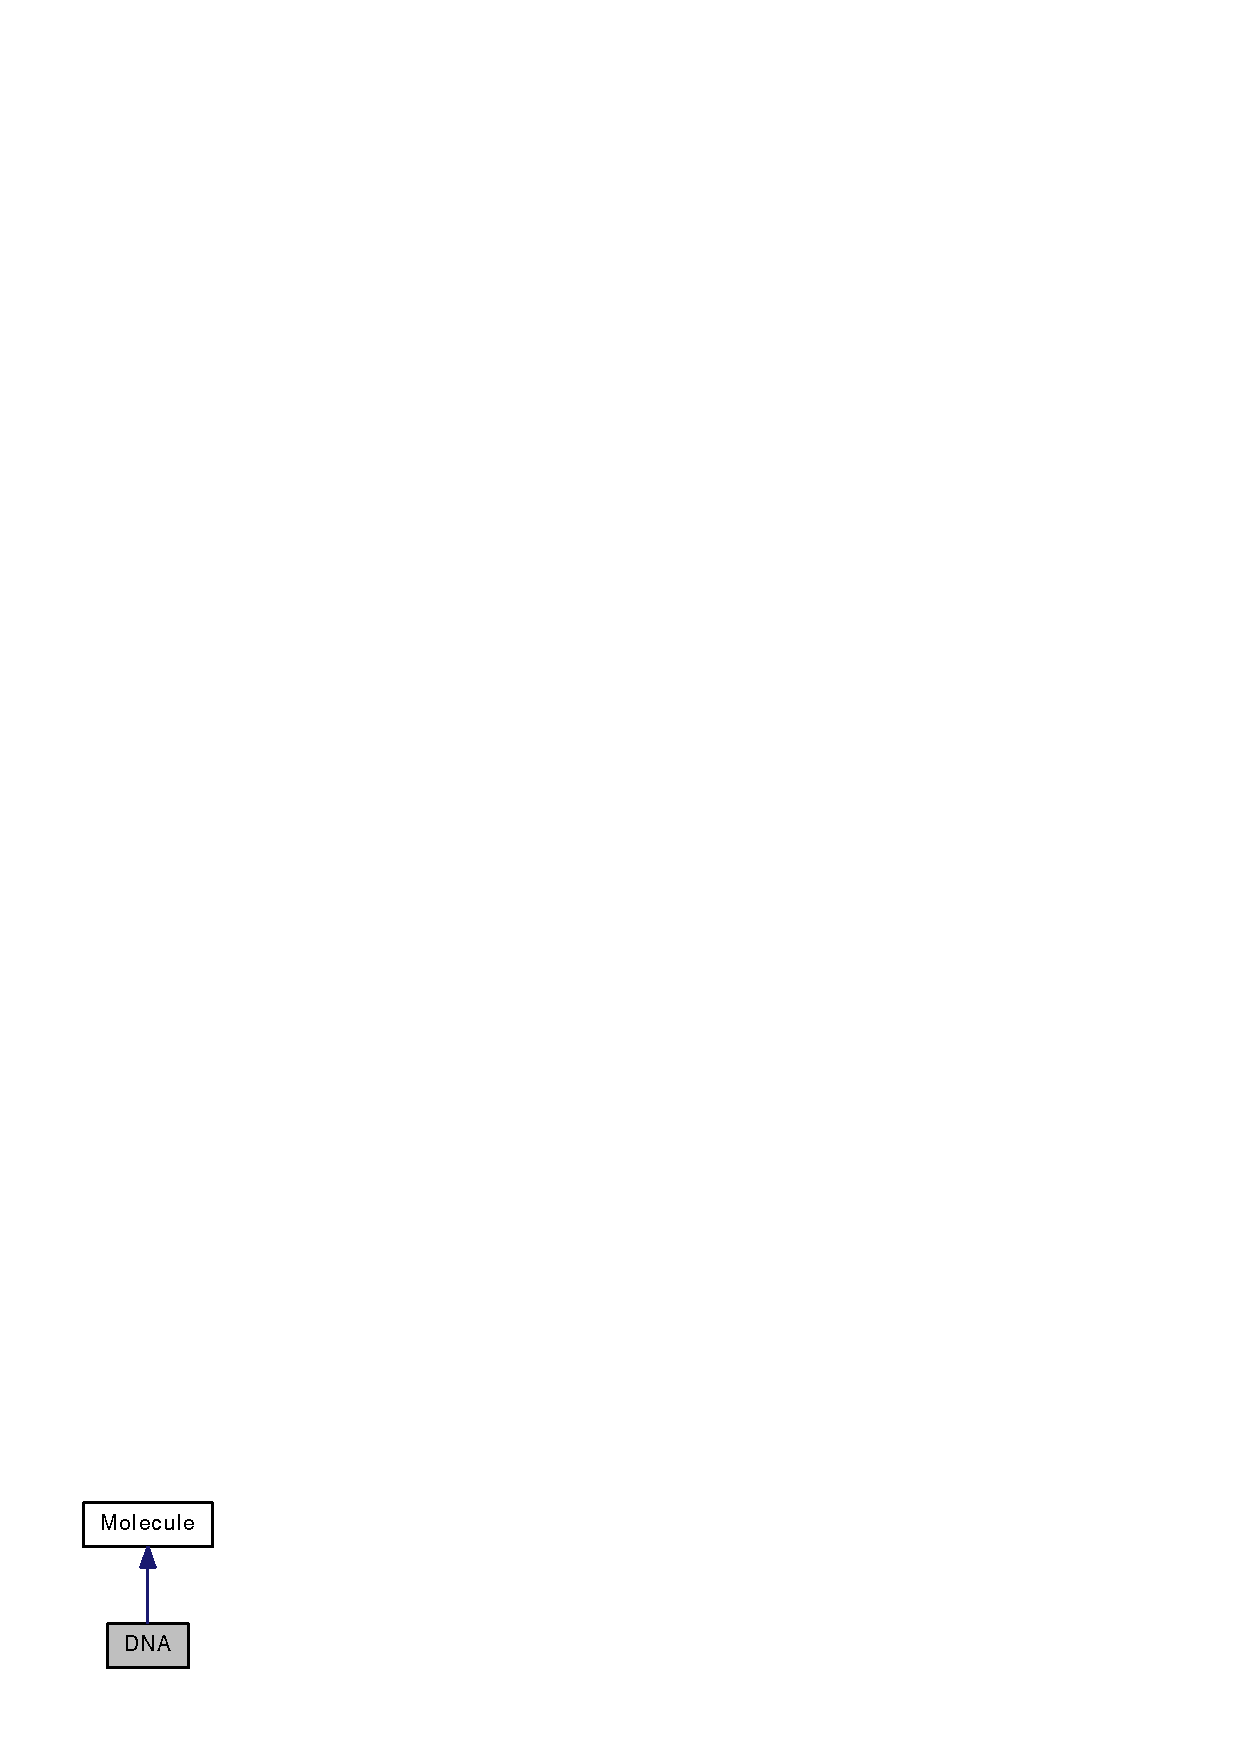
\includegraphics[width=106pt]{classDNA__inherit__graph}
\end{center}
\end{figure}
Collaboration diagram for DNA:\nopagebreak
\begin{figure}[H]
\begin{center}
\leavevmode
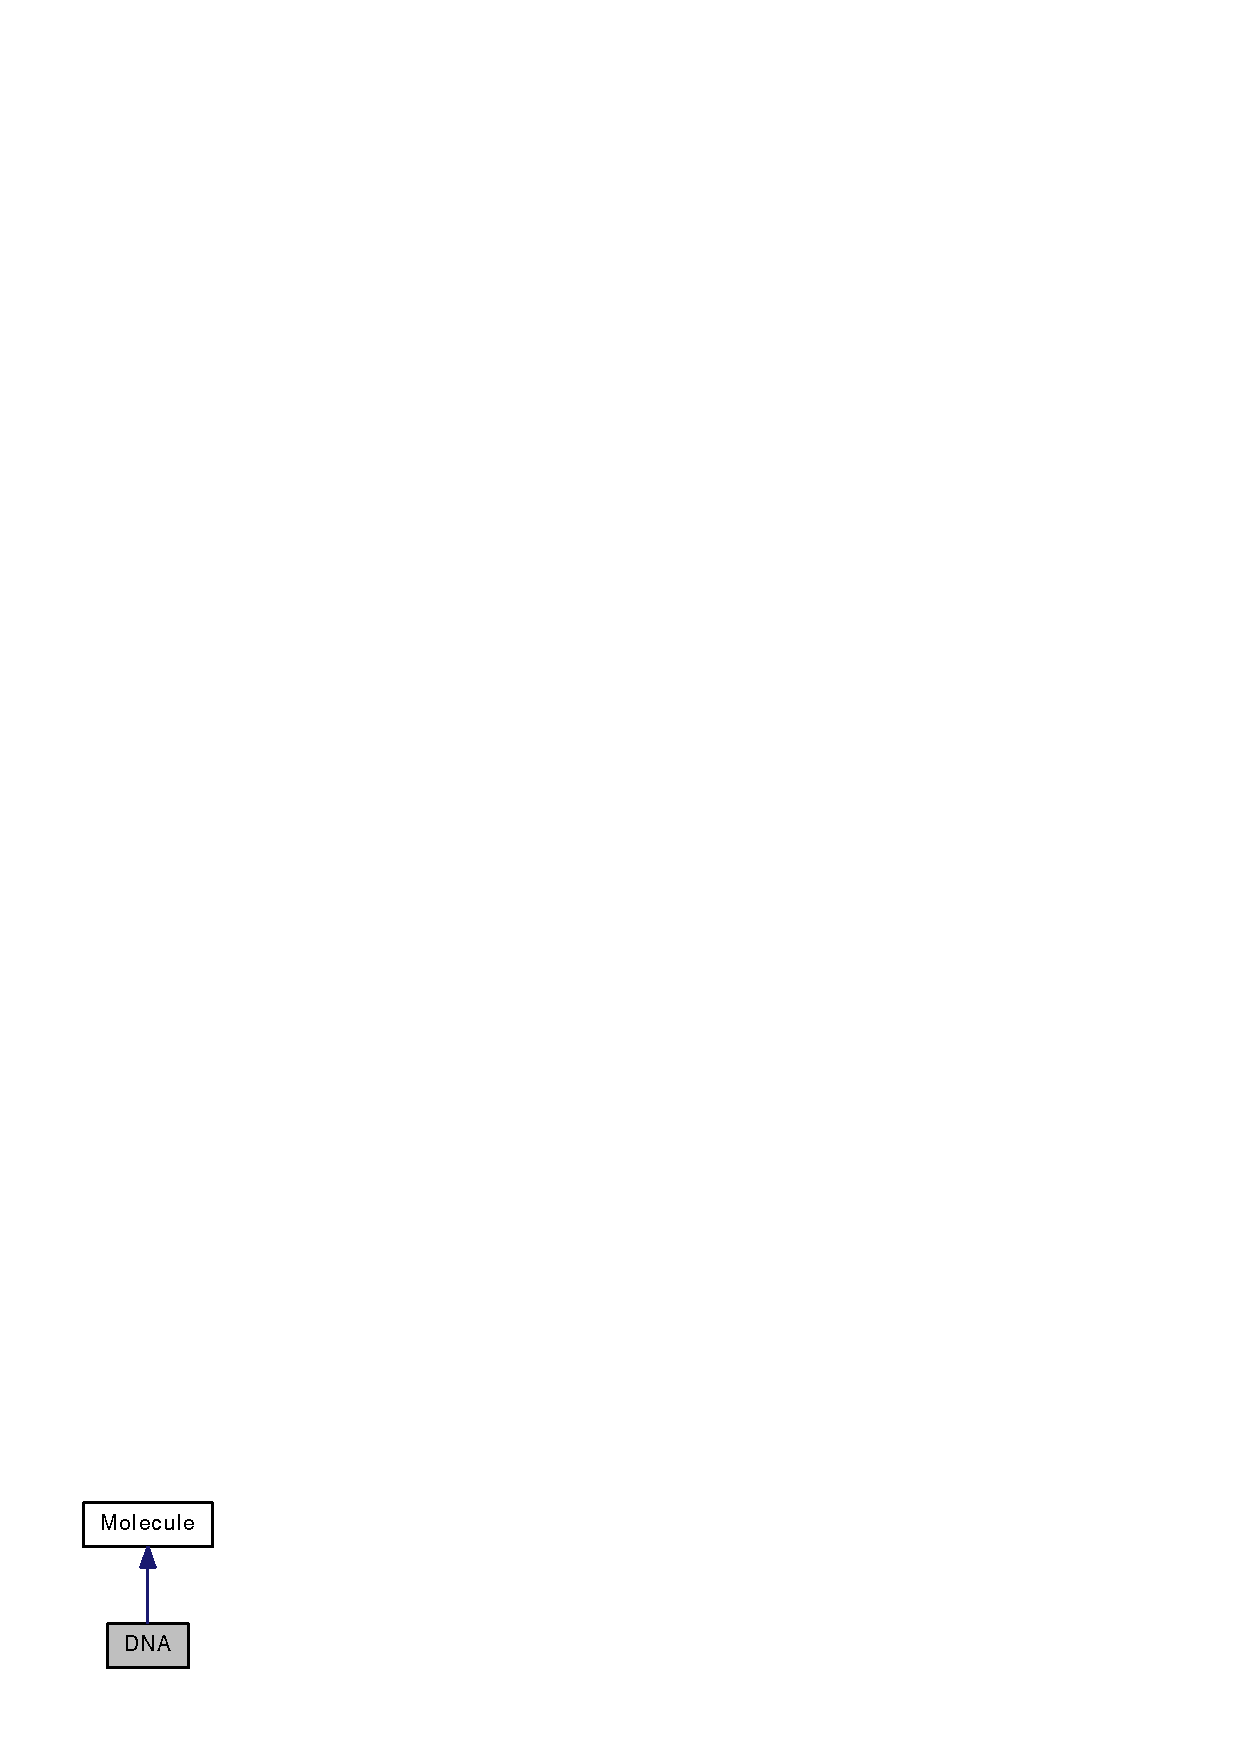
\includegraphics[width=106pt]{classDNA__coll__graph}
\end{center}
\end{figure}
\subsection*{Public Member Functions}
\begin{DoxyCompactItemize}
\item 
\hyperlink{classDNA_a3bad49a2b4f2afcc3a55f1d663e2d14e}{DNA} ()
\item 
\hyperlink{classDNA_ae839223a414026e083f5ba7491979e78}{$\sim$DNA} ()
\item 
float \hyperlink{classDNA_ac3f4ef00894483313ea44df6a85b3bab}{getValue} ()
\item 
float \hyperlink{classDNA_a10bec8cdc5922b2780887666c53891f1}{rkApprox} (int, float)
\item 
void \hyperlink{classDNA_aace4054119b4953683f23b2a0a9fd57c}{setHistoneModValue} (float)
\end{DoxyCompactItemize}
\subsection*{Public Attributes}
\begin{DoxyCompactItemize}
\item 
int \hyperlink{classDNA_a29696d77ea7eaabd48ee1d7eb9705b8e}{promoterId}
\item 
int \hyperlink{classDNA_a1c70e6e5beaf9ac5bfb9ab0d2cbf7f75}{hill}
\end{DoxyCompactItemize}


\subsection{Constructor \& Destructor Documentation}
\hypertarget{classDNA_a3bad49a2b4f2afcc3a55f1d663e2d14e}{
\index{DNA@{DNA}!DNA@{DNA}}
\index{DNA@{DNA}!DNA@{DNA}}
\subsubsection[{DNA}]{\setlength{\rightskip}{0pt plus 5cm}DNA::DNA ()}}
\label{classDNA_a3bad49a2b4f2afcc3a55f1d663e2d14e}
CustomMolecules implementation file.

Custom Molecules allow modification of the default behavior of molecules.

Each molecule must be defined in the \hyperlink{CustomMolecules_8h}{CustomMolecules.h} header file. \hyperlink{classDNA_a3bad49a2b4f2afcc3a55f1d663e2d14e}{DNA::DNA()}

Default Constructor

Derived from \hyperlink{classMolecule}{Molecule}. 

Here is the call graph for this function:\nopagebreak
\begin{figure}[H]
\begin{center}
\leavevmode
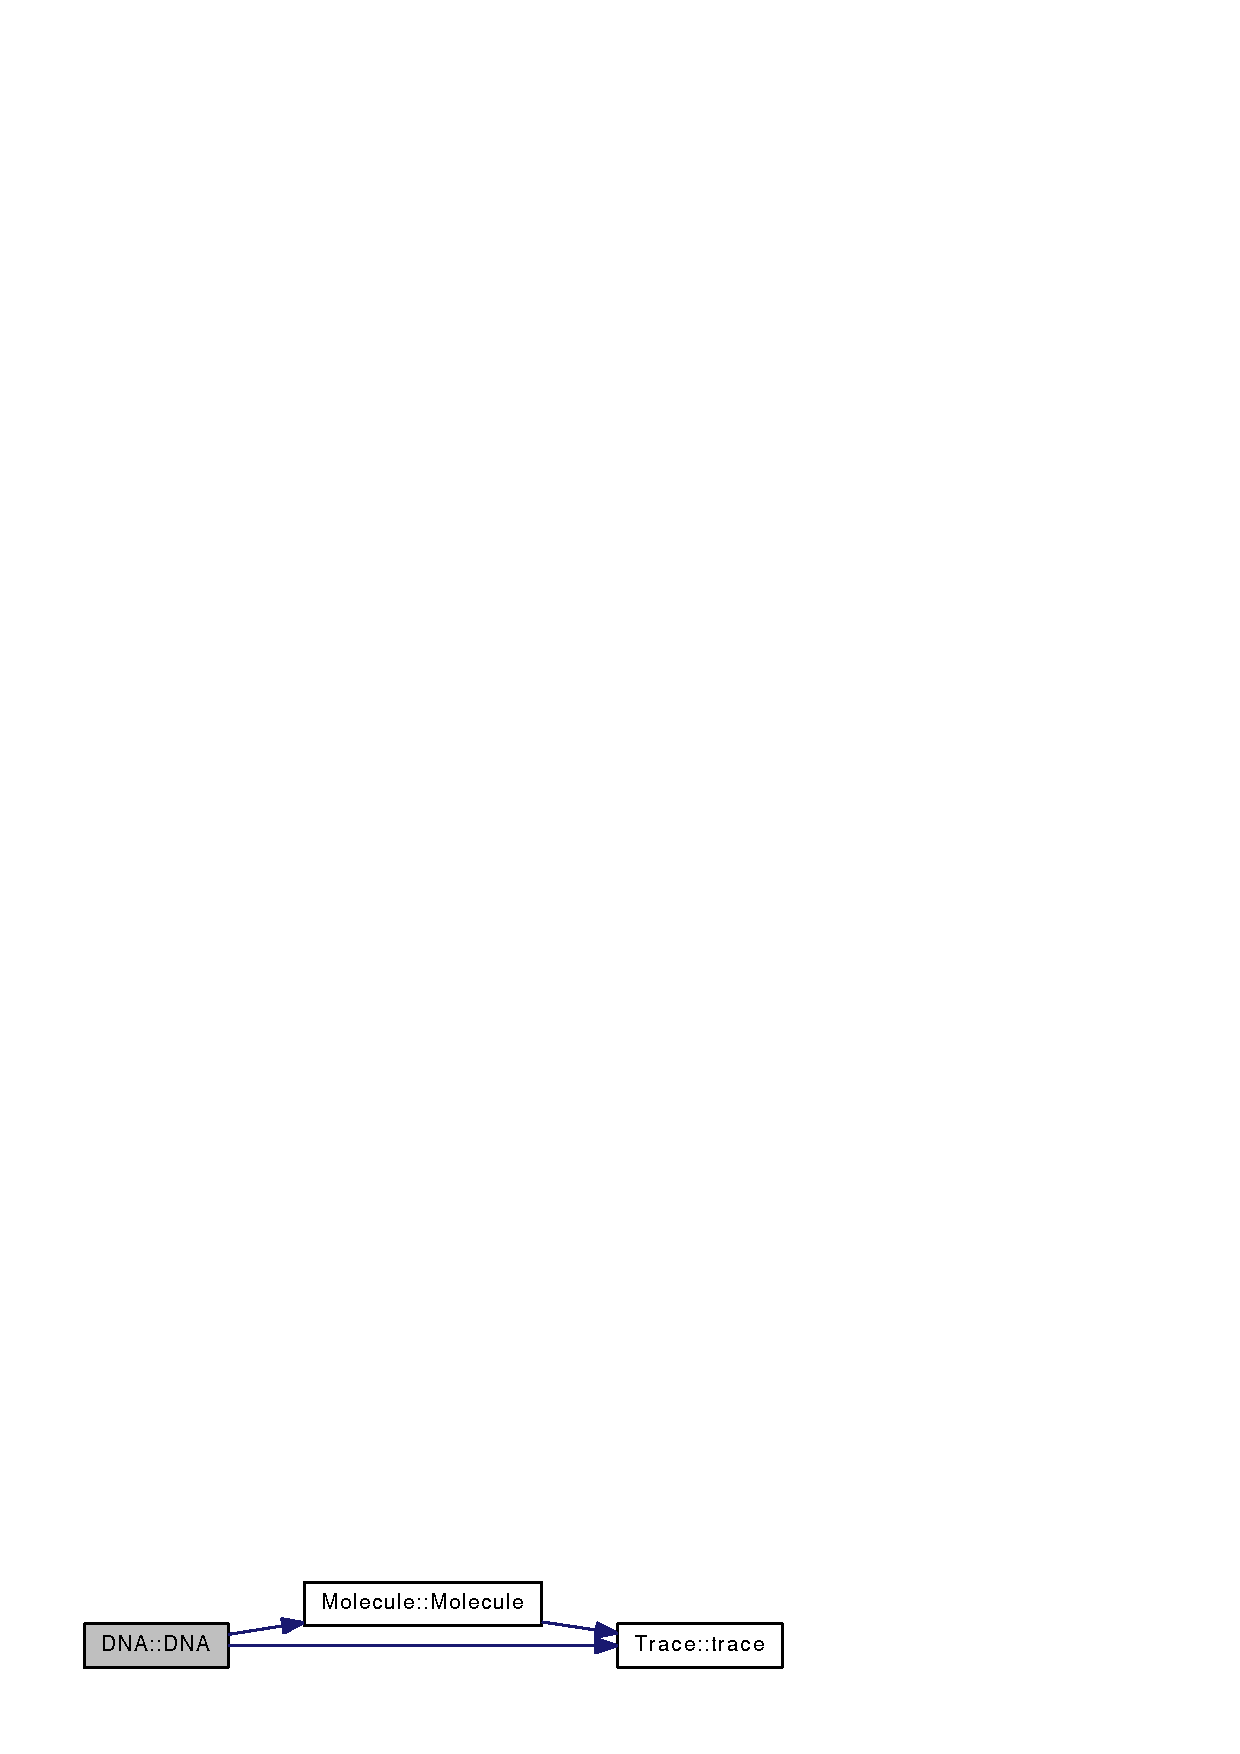
\includegraphics[width=190pt]{classDNA_a3bad49a2b4f2afcc3a55f1d663e2d14e_cgraph}
\end{center}
\end{figure}
\hypertarget{classDNA_ae839223a414026e083f5ba7491979e78}{
\index{DNA@{DNA}!$\sim$DNA@{$\sim$DNA}}
\index{$\sim$DNA@{$\sim$DNA}!DNA@{DNA}}
\subsubsection[{$\sim$DNA}]{\setlength{\rightskip}{0pt plus 5cm}DNA::$\sim$DNA ()}}
\label{classDNA_ae839223a414026e083f5ba7491979e78}
\hyperlink{classDNA_ae839223a414026e083f5ba7491979e78}{DNA::$\sim$DNA()}

Default Destructor 

\subsection{Member Function Documentation}
\hypertarget{classDNA_ac3f4ef00894483313ea44df6a85b3bab}{
\index{DNA@{DNA}!getValue@{getValue}}
\index{getValue@{getValue}!DNA@{DNA}}
\subsubsection[{getValue}]{\setlength{\rightskip}{0pt plus 5cm}float DNA::getValue ()\hspace{0.3cm}{\ttfamily  \mbox{[}virtual\mbox{]}}}}
\label{classDNA_ac3f4ef00894483313ea44df6a85b3bab}
Overload of virtual method \hyperlink{classMolecule_a554ea822918374775d5f52b5d49d8195}{Molecule::getValue}

\begin{DoxyReturn}{Returns}
Goodwin term describing the probability that the \hyperlink{classDNA}{DNA} is available for transcription. 
\end{DoxyReturn}


Reimplemented from \hyperlink{classMolecule_a554ea822918374775d5f52b5d49d8195}{Molecule}.\hypertarget{classDNA_a10bec8cdc5922b2780887666c53891f1}{
\index{DNA@{DNA}!rkApprox@{rkApprox}}
\index{rkApprox@{rkApprox}!DNA@{DNA}}
\subsubsection[{rkApprox}]{\setlength{\rightskip}{0pt plus 5cm}float DNA::rkApprox (int {\em rkIteration}, \/  float {\em rkStepSize})\hspace{0.3cm}{\ttfamily  \mbox{[}virtual\mbox{]}}}}
\label{classDNA_a10bec8cdc5922b2780887666c53891f1}
float \hyperlink{classMolecule_adabb58a65655a7f55dae0d82b65d04ba}{Molecule::rkApprox(int, float)} (Virtual Function)

Returns the next approximate value of this molecule for the next timestep for the specified stage of Runge-\/Kutta. Runge-\/Kutta uses successive iterations to make more accurate approximations of a solution.

rkApprox should be used in \hyperlink{classInteraction_a6328831e714adf9c8177f6052d2e017f}{Interaction::getEffect}, to provide the Runge-\/Kutta corrected concentrations of molecules during runge-\/kutta calculation instead of the base value for all iterations.


\begin{DoxyParams}{Parameters}
\item[{\em rkIteration}]the current iteration of Runge-\/Kutta \item[{\em rkStepSize}]the timestep being used by Runge-\/Kutta \end{DoxyParams}


Reimplemented from \hyperlink{classMolecule_adabb58a65655a7f55dae0d82b65d04ba}{Molecule}.

Here is the call graph for this function:\nopagebreak
\begin{figure}[H]
\begin{center}
\leavevmode
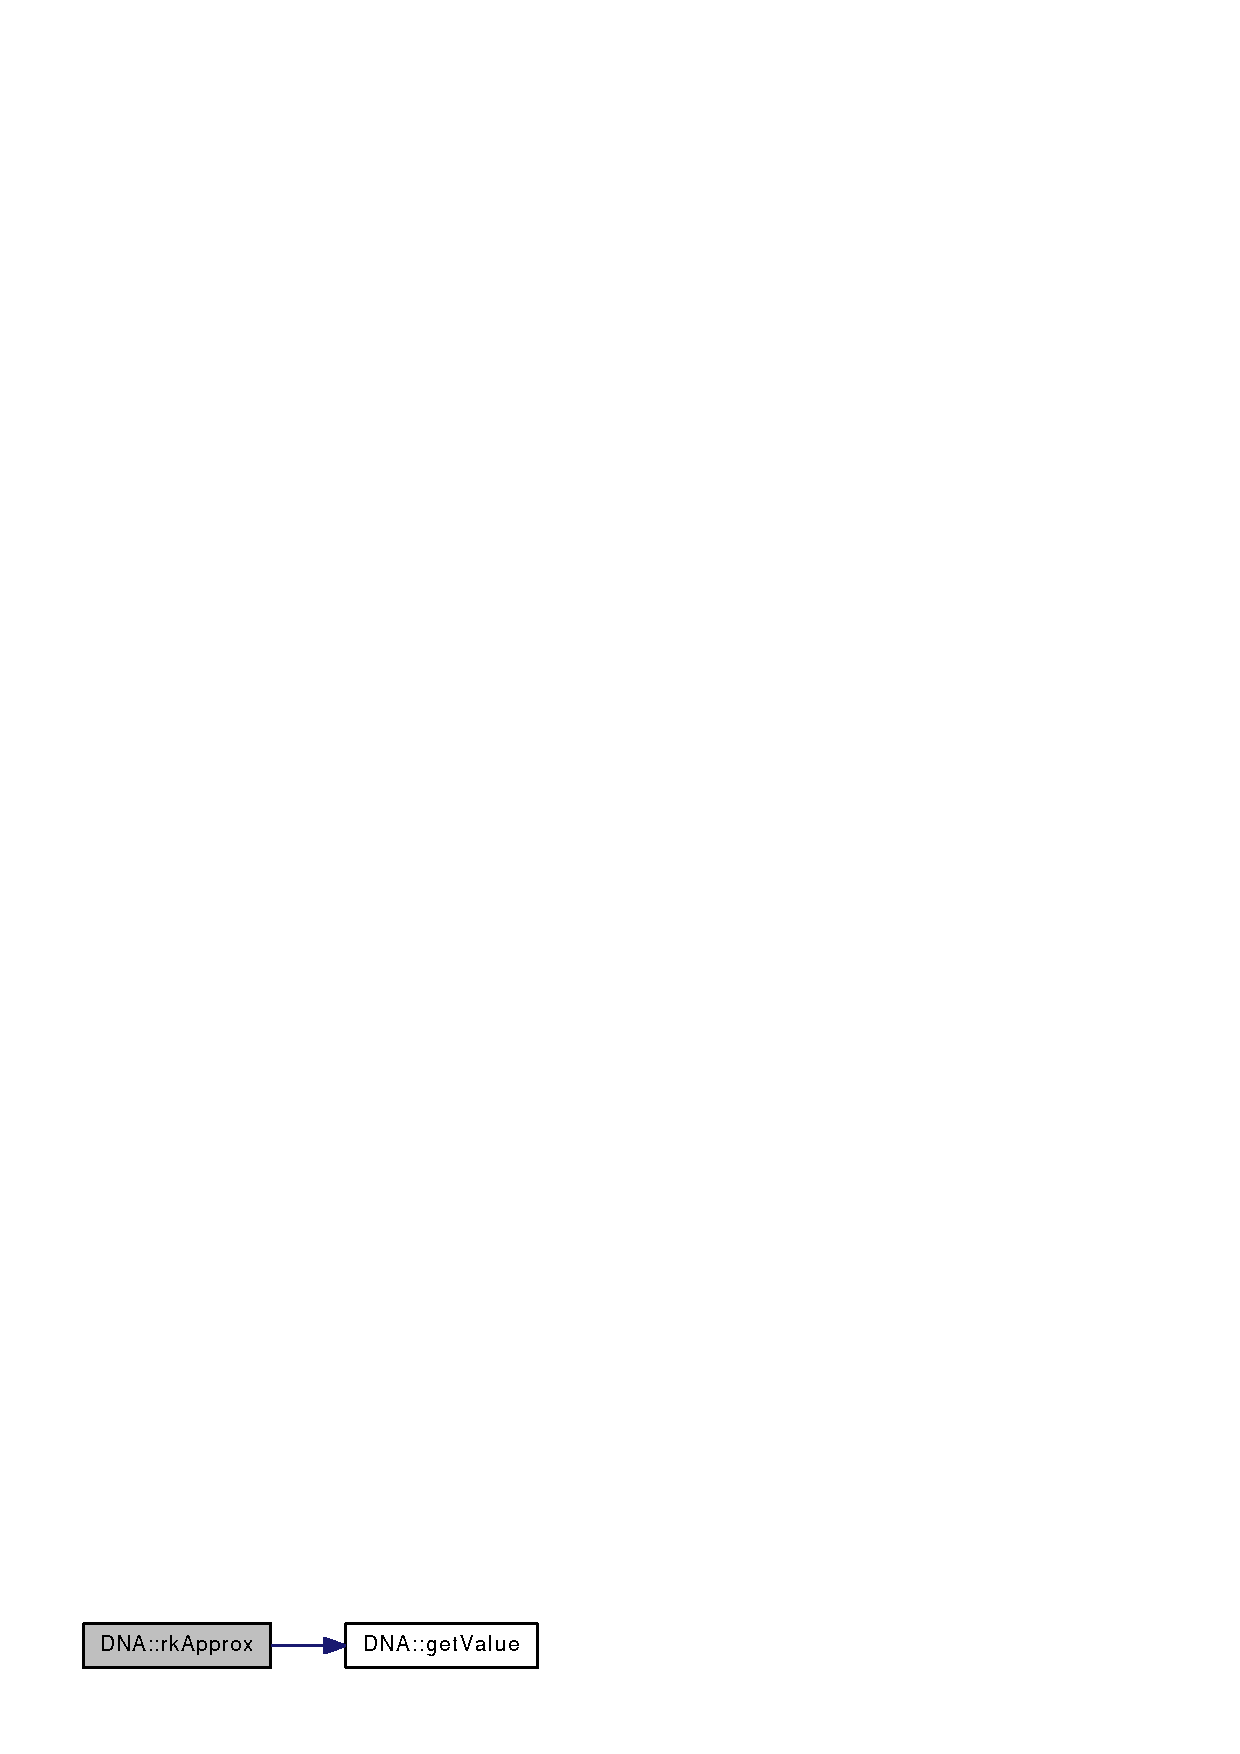
\includegraphics[width=131pt]{classDNA_a10bec8cdc5922b2780887666c53891f1_cgraph}
\end{center}
\end{figure}
\hypertarget{classDNA_aace4054119b4953683f23b2a0a9fd57c}{
\index{DNA@{DNA}!setHistoneModValue@{setHistoneModValue}}
\index{setHistoneModValue@{setHistoneModValue}!DNA@{DNA}}
\subsubsection[{setHistoneModValue}]{\setlength{\rightskip}{0pt plus 5cm}void DNA::setHistoneModValue (float {\em newVal})}}
\label{classDNA_aace4054119b4953683f23b2a0a9fd57c}


\subsection{Member Data Documentation}
\hypertarget{classDNA_a1c70e6e5beaf9ac5bfb9ab0d2cbf7f75}{
\index{DNA@{DNA}!hill@{hill}}
\index{hill@{hill}!DNA@{DNA}}
\subsubsection[{hill}]{\setlength{\rightskip}{0pt plus 5cm}int {\bf DNA::hill}}}
\label{classDNA_a1c70e6e5beaf9ac5bfb9ab0d2cbf7f75}
\hypertarget{classDNA_a29696d77ea7eaabd48ee1d7eb9705b8e}{
\index{DNA@{DNA}!promoterId@{promoterId}}
\index{promoterId@{promoterId}!DNA@{DNA}}
\subsubsection[{promoterId}]{\setlength{\rightskip}{0pt plus 5cm}int {\bf DNA::promoterId}}}
\label{classDNA_a29696d77ea7eaabd48ee1d7eb9705b8e}


The documentation for this class was generated from the following files:\begin{DoxyCompactItemize}
\item 
\hyperlink{CustomMolecules_8h}{CustomMolecules.h}\item 
\hyperlink{CustomMolecules_8cpp}{CustomMolecules.cpp}\end{DoxyCompactItemize}

\hypertarget{classExperiment}{
\section{Experiment Class Reference}
\label{classExperiment}\index{Experiment@{Experiment}}
}


{\ttfamily \#include $<$Experiment.h$>$}\subsection*{Public Member Functions}
\begin{DoxyCompactItemize}
\item 
\hyperlink{classExperiment_a600bd431197ce5df6c62f6647c561f7b}{Experiment} (int ncells, int generations, int max\_\-basic, int max\_\-ptm, int max\_\-comp, int max\_\-prom, float min\_\-kinetic\_\-rate, float max\_\-kinetic\_\-rate, float rk\_\-time\_\-limit, float rk\_\-time\_\-step, float initial\_\-conc)
\item 
\hyperlink{classExperiment_a96058d848040e45948bbb60623711da6}{$\sim$Experiment} ()
\item 
void \hyperlink{classExperiment_ab15fca04be9b7bcad65b264b23b4a499}{start} ()
\item 
void \hyperlink{classExperiment_a7597c63f9fe2f8dede62dbe79202bf61}{setOutputOptions} (int, int, int, int)
\end{DoxyCompactItemize}


\subsection{Constructor \& Destructor Documentation}
\hypertarget{classExperiment_a600bd431197ce5df6c62f6647c561f7b}{
\index{Experiment@{Experiment}!Experiment@{Experiment}}
\index{Experiment@{Experiment}!Experiment@{Experiment}}
\subsubsection[{Experiment}]{\setlength{\rightskip}{0pt plus 5cm}Experiment::Experiment (int {\em ncells}, \/  int {\em generations}, \/  int {\em max\_\-basic}, \/  int {\em max\_\-ptm}, \/  int {\em max\_\-comp}, \/  int {\em max\_\-prom}, \/  float {\em min\_\-kinetic\_\-rate}, \/  float {\em max\_\-kinetic\_\-rate}, \/  float {\em rk\_\-time\_\-limit}, \/  float {\em rk\_\-time\_\-step}, \/  float {\em initial\_\-conc})}}
\label{classExperiment_a600bd431197ce5df6c62f6647c561f7b}
Experiment::Experiment(int, int)

\hyperlink{classExperiment}{Experiment} constructor.


\begin{DoxyParams}{Parameters}
\item[{\em ncells}]number of \hyperlink{classCell}{Cell} objects to be created. \item[{\em generations}]number of Generations the \hyperlink{classExperiment}{Experiment} will run for. \item[{\em max\_\-basic}]maximum number of basic proteins allowed in each \hyperlink{classCell}{Cell} \item[{\em max\_\-ptm}]maximum number of PTM proteins allowed in each \hyperlink{classCell}{Cell} \item[{\em max\_\-comp}]maximum number of complexed proteins allowed in each \hyperlink{classCell}{Cell} \item[{\em max\_\-prom}]maximum number of protein-\/promoter interactions allowed in each cell \item[{\em min\_\-kinetic\_\-rate}]the lower bound on randomly generated kinetic rates \item[{\em max\_\-kinetic\_\-rate}]the upper bound on randomly generated kinetic rates \item[{\em rk\_\-time\_\-limit}]the stopping condition for runge-\/kutta iteration \item[{\em rk\_\-time\_\-step}]how much time to advance each iteration \item[{\em initial\_\-conc}]the initial concentration for molecules \end{DoxyParams}


Here is the call graph for this function:\nopagebreak
\begin{figure}[H]
\begin{center}
\leavevmode
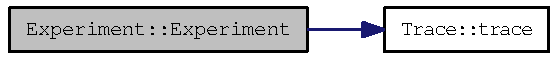
\includegraphics[width=152pt]{classExperiment_a600bd431197ce5df6c62f6647c561f7b_cgraph}
\end{center}
\end{figure}
\hypertarget{classExperiment_a96058d848040e45948bbb60623711da6}{
\index{Experiment@{Experiment}!$\sim$Experiment@{$\sim$Experiment}}
\index{$\sim$Experiment@{$\sim$Experiment}!Experiment@{Experiment}}
\subsubsection[{$\sim$Experiment}]{\setlength{\rightskip}{0pt plus 5cm}Experiment::$\sim$Experiment ()}}
\label{classExperiment_a96058d848040e45948bbb60623711da6}
Experiment::$\sim$Experiment(int, int)

\hyperlink{classExperiment}{Experiment} destructor.

Deletes the \hyperlink{classCell}{Cell} objects from the cells vector, then deletes the vector itself. 

Here is the call graph for this function:\nopagebreak
\begin{figure}[H]
\begin{center}
\leavevmode
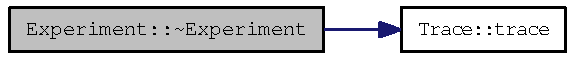
\includegraphics[width=156pt]{classExperiment_a96058d848040e45948bbb60623711da6_cgraph}
\end{center}
\end{figure}


\subsection{Member Function Documentation}
\hypertarget{classExperiment_a7597c63f9fe2f8dede62dbe79202bf61}{
\index{Experiment@{Experiment}!setOutputOptions@{setOutputOptions}}
\index{setOutputOptions@{setOutputOptions}!Experiment@{Experiment}}
\subsubsection[{setOutputOptions}]{\setlength{\rightskip}{0pt plus 5cm}void Experiment::setOutputOptions (int {\em gv\_\-flag}, \/  int {\em gp\_\-flag}, \/  int {\em eachgen\_\-flag}, \/  int {\em scoring\_\-interval})}}
\label{classExperiment_a7597c63f9fe2f8dede62dbe79202bf61}
\hypertarget{classExperiment_ab15fca04be9b7bcad65b264b23b4a499}{
\index{Experiment@{Experiment}!start@{start}}
\index{start@{start}!Experiment@{Experiment}}
\subsubsection[{start}]{\setlength{\rightskip}{0pt plus 5cm}void Experiment::start ()}}
\label{classExperiment_ab15fca04be9b7bcad65b264b23b4a499}


Here is the call graph for this function:\nopagebreak
\begin{figure}[H]
\begin{center}
\leavevmode
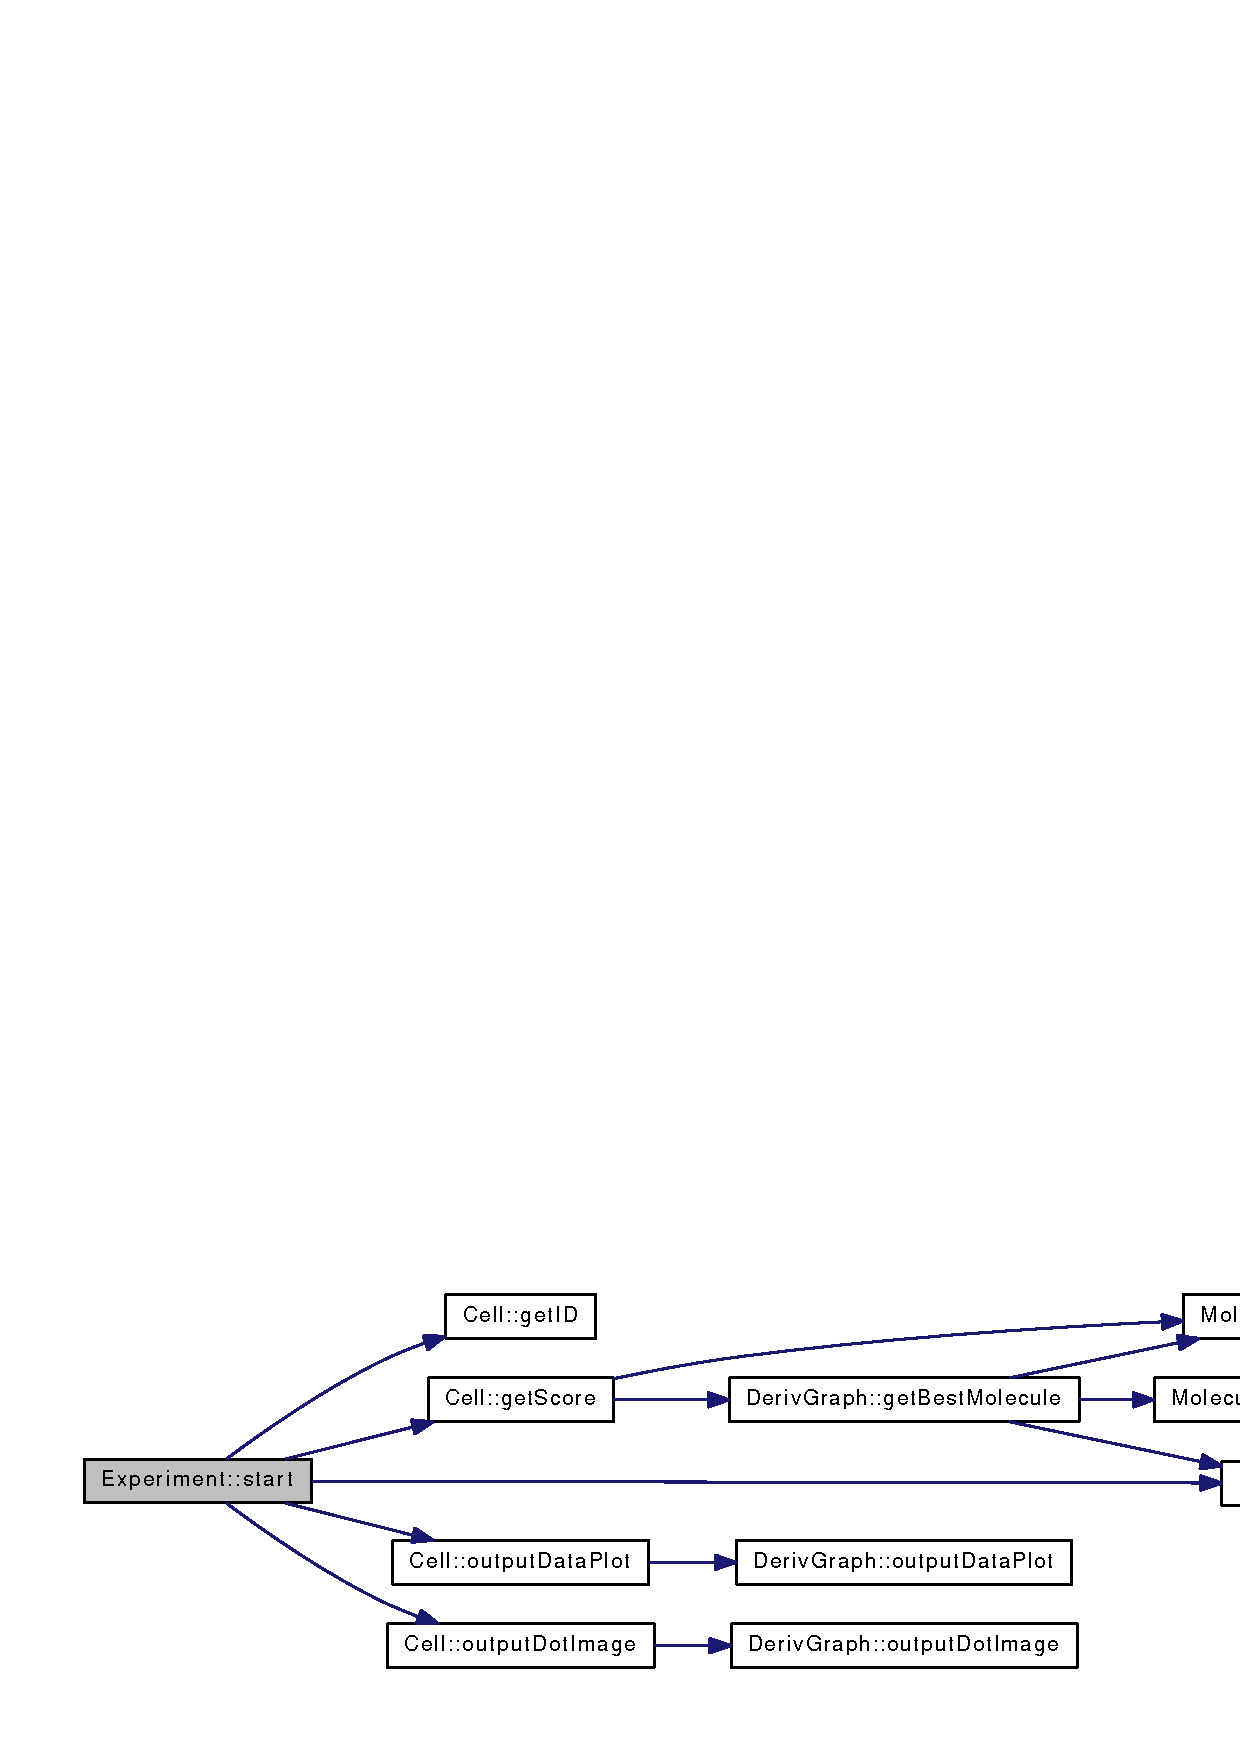
\includegraphics[width=351pt]{classExperiment_ab15fca04be9b7bcad65b264b23b4a499_cgraph}
\end{center}
\end{figure}


The documentation for this class was generated from the following files:\begin{DoxyCompactItemize}
\item 
\hyperlink{Experiment_8h}{Experiment.h}\item 
\hyperlink{Experiment_8cpp}{Experiment.cpp}\end{DoxyCompactItemize}

\hypertarget{classForwardComplexation}{
\section{ForwardComplexation Class Reference}
\label{classForwardComplexation}\index{ForwardComplexation@{ForwardComplexation}}
}


{\ttfamily \#include $<$CustomInteractions.h$>$}Inheritance diagram for ForwardComplexation:\nopagebreak
\begin{figure}[H]
\begin{center}
\leavevmode
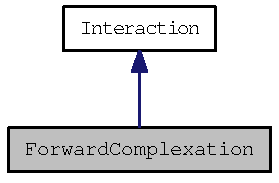
\includegraphics[width=170pt]{classForwardComplexation__inherit__graph}
\end{center}
\end{figure}
Collaboration diagram for ForwardComplexation:\nopagebreak
\begin{figure}[H]
\begin{center}
\leavevmode
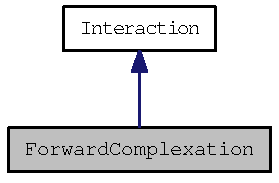
\includegraphics[width=170pt]{classForwardComplexation__coll__graph}
\end{center}
\end{figure}
\subsection*{Public Member Functions}
\begin{DoxyCompactItemize}
\item 
\hyperlink{classForwardComplexation_a0ab16d0c2ad4bef757d811d4b7fd9682}{ForwardComplexation} (int, int)
\item 
\hyperlink{classForwardComplexation_afd5c904c0ae1842caa2e26162300d2ff}{$\sim$ForwardComplexation} ()
\item 
virtual float \hyperlink{classForwardComplexation_a8f7f867b98b484ed0f09192ebd280e1a}{getEffect} (ListDigraph $\ast$, ListDigraph::NodeMap$<$ \hyperlink{classMolecule}{Molecule} $\ast$ $>$ $\ast$, ListDigraph::ArcMap$<$ \hyperlink{classInteraction}{Interaction} $\ast$ $>$ $\ast$, ListDigraph::Node, int, float)
\end{DoxyCompactItemize}
\subsection*{Public Attributes}
\begin{DoxyCompactItemize}
\item 
int \hyperlink{classForwardComplexation_ab8992a599d764810b7be577f88ee791c}{firstNodeID}
\item 
int \hyperlink{classForwardComplexation_a48ebe46e9ee3b749165649d8b14c33fc}{secondNodeID}
\end{DoxyCompactItemize}


\subsection{Constructor \& Destructor Documentation}
\hypertarget{classForwardComplexation_a0ab16d0c2ad4bef757d811d4b7fd9682}{
\index{ForwardComplexation@{ForwardComplexation}!ForwardComplexation@{ForwardComplexation}}
\index{ForwardComplexation@{ForwardComplexation}!ForwardComplexation@{ForwardComplexation}}
\subsubsection[{ForwardComplexation}]{\setlength{\rightskip}{0pt plus 5cm}ForwardComplexation::ForwardComplexation (int {\em n1}, \/  int {\em n2})}}
\label{classForwardComplexation_a0ab16d0c2ad4bef757d811d4b7fd9682}


Here is the call graph for this function:\nopagebreak
\begin{figure}[H]
\begin{center}
\leavevmode
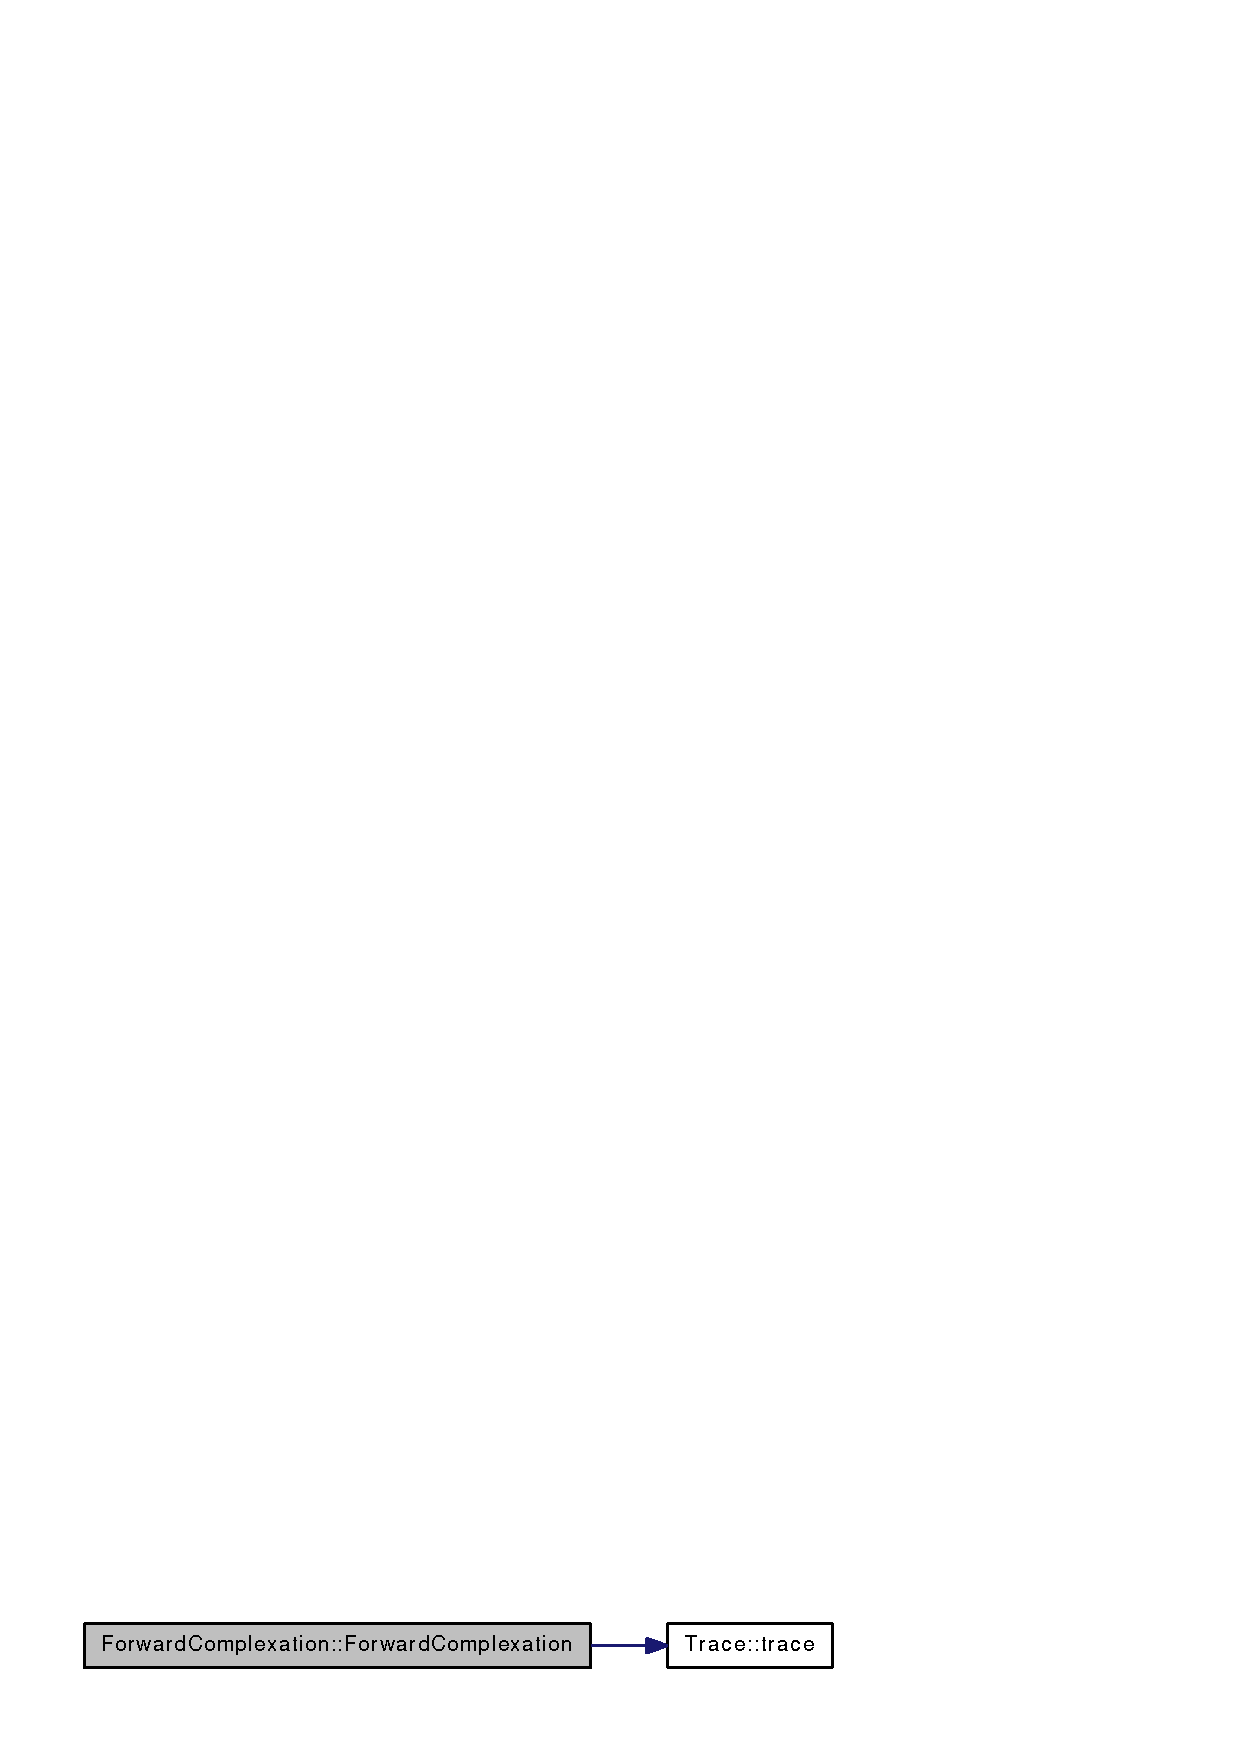
\includegraphics[width=202pt]{classForwardComplexation_a0ab16d0c2ad4bef757d811d4b7fd9682_cgraph}
\end{center}
\end{figure}
\hypertarget{classForwardComplexation_afd5c904c0ae1842caa2e26162300d2ff}{
\index{ForwardComplexation@{ForwardComplexation}!$\sim$ForwardComplexation@{$\sim$ForwardComplexation}}
\index{$\sim$ForwardComplexation@{$\sim$ForwardComplexation}!ForwardComplexation@{ForwardComplexation}}
\subsubsection[{$\sim$ForwardComplexation}]{\setlength{\rightskip}{0pt plus 5cm}ForwardComplexation::$\sim$ForwardComplexation ()}}
\label{classForwardComplexation_afd5c904c0ae1842caa2e26162300d2ff}


\subsection{Member Function Documentation}
\hypertarget{classForwardComplexation_a8f7f867b98b484ed0f09192ebd280e1a}{
\index{ForwardComplexation@{ForwardComplexation}!getEffect@{getEffect}}
\index{getEffect@{getEffect}!ForwardComplexation@{ForwardComplexation}}
\subsubsection[{getEffect}]{\setlength{\rightskip}{0pt plus 5cm}float ForwardComplexation::getEffect (ListDigraph $\ast$ {\em g}, \/  ListDigraph::NodeMap$<$ {\bf Molecule} $\ast$ $>$ $\ast$ {\em m}, \/  ListDigraph::ArcMap$<$ {\bf Interaction} $\ast$ $>$ $\ast$ {\em i}, \/  ListDigraph::Node {\em a}, \/  int {\em rkIter}, \/  float {\em rkStep})\hspace{0.3cm}{\ttfamily  \mbox{[}virtual\mbox{]}}}}
\label{classForwardComplexation_a8f7f867b98b484ed0f09192ebd280e1a}
float Interaction::getEffect(ListDigraph$\ast$ , NodeMap$<$Molecule$\ast$$>$$\ast$ , ArcMap$<$Interaction$\ast$$>$$\ast$ , Node , int, float)

Get the effect this interaction has on a particular node.

This method defines the behavior of an interaction which connects two molecules. The effect on Node a can be dependent on any other molecule, which can be accessed using the ListDigraph, NodeMap, and ArcMap parameters.

Runge-\/Kutta iteratively approximates the change in concentration during a given timestep. The first iteration is based soley on the current concentration, and each further iteration takes the result of the previous iteration into account. The Runge-\/Kutta data are stored in each molecule, and it is necessary to call Molecule::rkApprox(stepsize, iteration) rather than \hyperlink{classMolecule_a554ea822918374775d5f52b5d49d8195}{Molecule::getValue()} to get the current Iteration's approximated concentration.


\begin{DoxyParams}{Parameters}
\item[{\em g}]The graph object containing Node-\/Node relationships. \item[{\em m}]The NodeMap object containing Node-\/Molecule mappings. \item[{\em i}]The ArcMap object containing Arc-\/Interaction mappings. \item[{\em a}]The Node to calculate the effect for \item[{\em rkIter}]The current iteration of Runge-\/Kutta \mbox{[}0,3\mbox{]} \item[{\em rkStep}]The stepsize of Runge-\/Kutta \end{DoxyParams}


Reimplemented from \hyperlink{classInteraction_a6328831e714adf9c8177f6052d2e017f}{Interaction}.

Here is the call graph for this function:\nopagebreak
\begin{figure}[H]
\begin{center}
\leavevmode
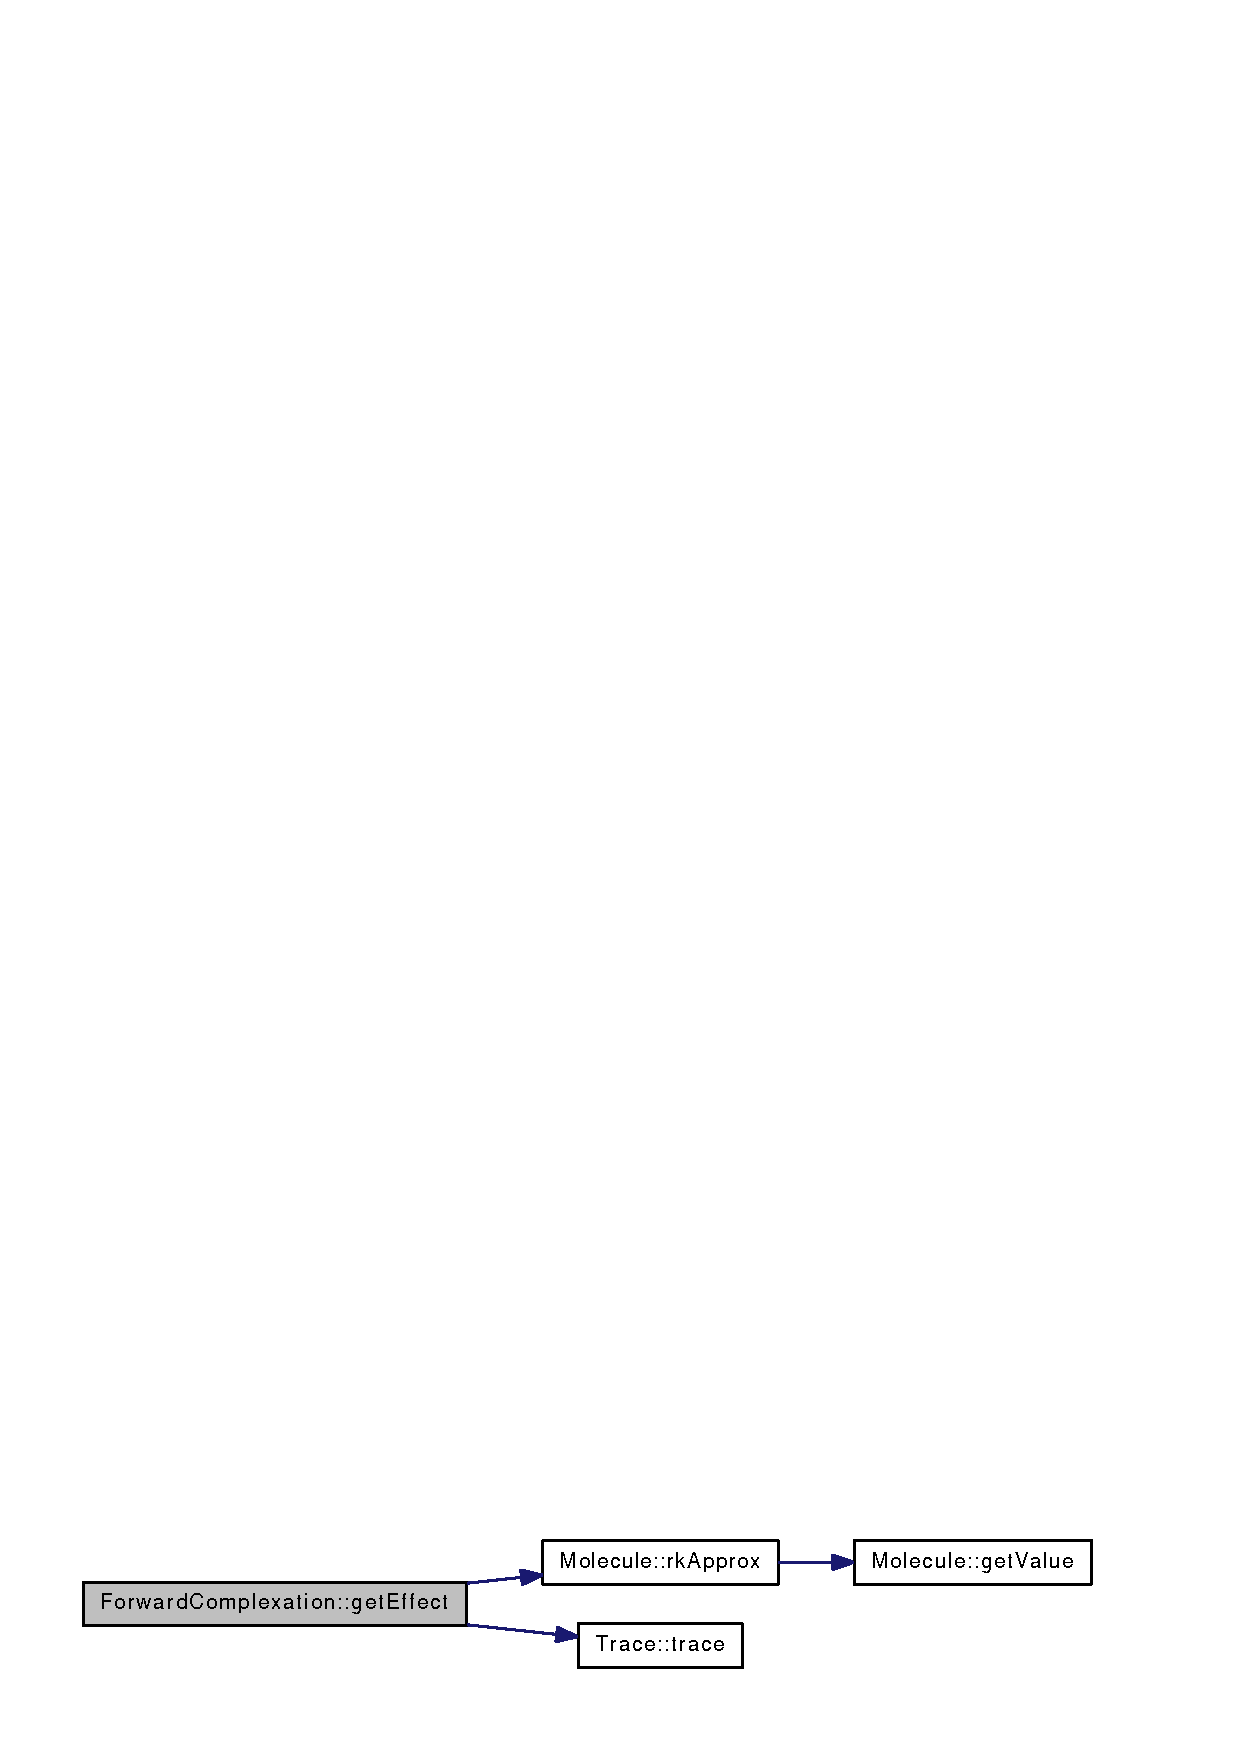
\includegraphics[width=264pt]{classForwardComplexation_a8f7f867b98b484ed0f09192ebd280e1a_cgraph}
\end{center}
\end{figure}


\subsection{Member Data Documentation}
\hypertarget{classForwardComplexation_ab8992a599d764810b7be577f88ee791c}{
\index{ForwardComplexation@{ForwardComplexation}!firstNodeID@{firstNodeID}}
\index{firstNodeID@{firstNodeID}!ForwardComplexation@{ForwardComplexation}}
\subsubsection[{firstNodeID}]{\setlength{\rightskip}{0pt plus 5cm}int {\bf ForwardComplexation::firstNodeID}}}
\label{classForwardComplexation_ab8992a599d764810b7be577f88ee791c}
\hypertarget{classForwardComplexation_a48ebe46e9ee3b749165649d8b14c33fc}{
\index{ForwardComplexation@{ForwardComplexation}!secondNodeID@{secondNodeID}}
\index{secondNodeID@{secondNodeID}!ForwardComplexation@{ForwardComplexation}}
\subsubsection[{secondNodeID}]{\setlength{\rightskip}{0pt plus 5cm}int {\bf ForwardComplexation::secondNodeID}}}
\label{classForwardComplexation_a48ebe46e9ee3b749165649d8b14c33fc}


The documentation for this class was generated from the following files:\begin{DoxyCompactItemize}
\item 
\hyperlink{CustomInteractions_8h}{CustomInteractions.h}\item 
\hyperlink{CustomInteractions_8cpp}{CustomInteractions.cpp}\end{DoxyCompactItemize}

\hypertarget{classForwardPTM}{
\section{ForwardPTM Class Reference}
\label{classForwardPTM}\index{ForwardPTM@{ForwardPTM}}
}


{\ttfamily \#include $<$CustomInteractions.h$>$}Inheritance diagram for ForwardPTM:\nopagebreak
\begin{figure}[H]
\begin{center}
\leavevmode
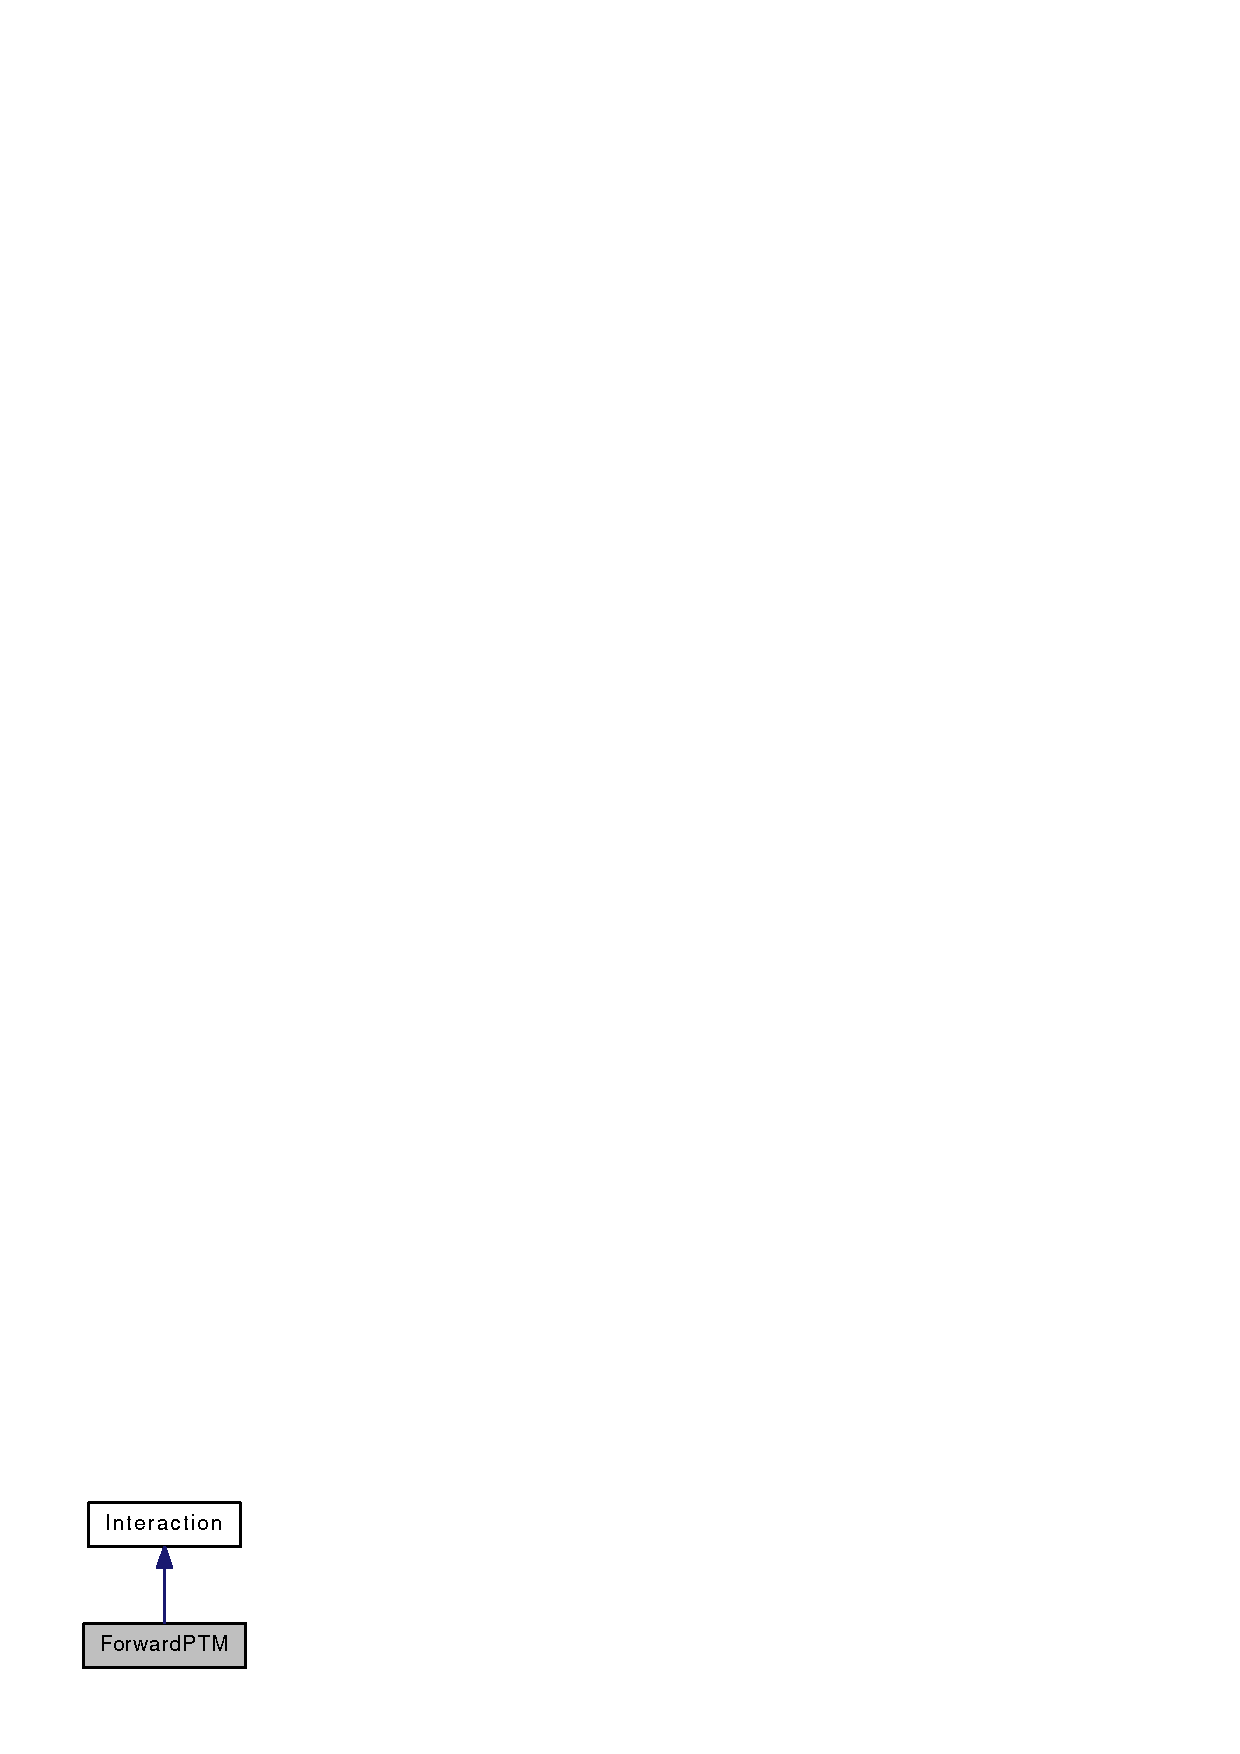
\includegraphics[width=122pt]{classForwardPTM__inherit__graph}
\end{center}
\end{figure}
Collaboration diagram for ForwardPTM:\nopagebreak
\begin{figure}[H]
\begin{center}
\leavevmode
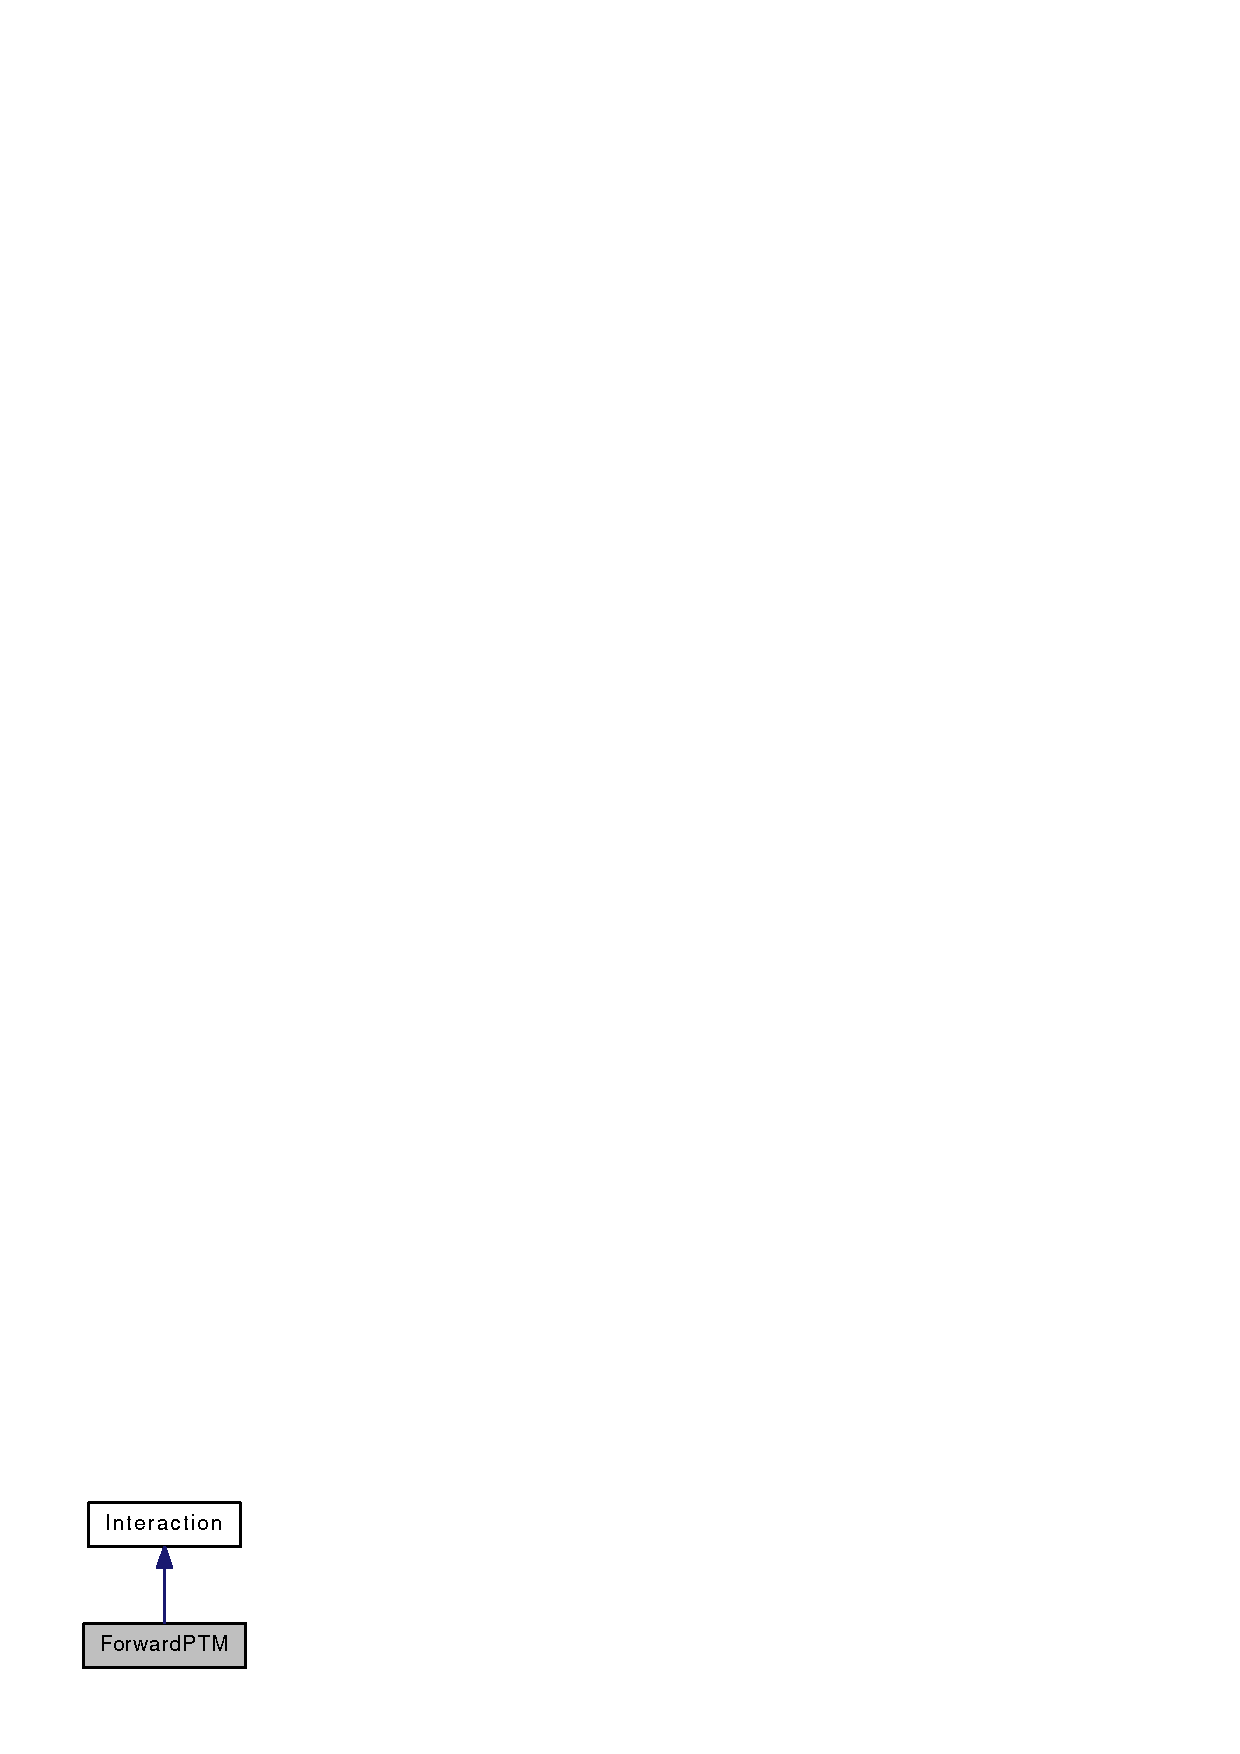
\includegraphics[width=122pt]{classForwardPTM__coll__graph}
\end{center}
\end{figure}
\subsection*{Public Member Functions}
\begin{DoxyCompactItemize}
\item 
\hyperlink{classForwardPTM_a42913d0481561a489b8664cd22cf7b0c}{ForwardPTM} ()
\item 
\hyperlink{classForwardPTM_a9fa8aa77099a6bb8d4fbe326a5d84704}{$\sim$ForwardPTM} ()
\end{DoxyCompactItemize}


\subsection{Constructor \& Destructor Documentation}
\hypertarget{classForwardPTM_a42913d0481561a489b8664cd22cf7b0c}{
\index{ForwardPTM@{ForwardPTM}!ForwardPTM@{ForwardPTM}}
\index{ForwardPTM@{ForwardPTM}!ForwardPTM@{ForwardPTM}}
\subsubsection[{ForwardPTM}]{\setlength{\rightskip}{0pt plus 5cm}ForwardPTM::ForwardPTM ()}}
\label{classForwardPTM_a42913d0481561a489b8664cd22cf7b0c}


Here is the call graph for this function:\nopagebreak
\begin{figure}[H]
\begin{center}
\leavevmode
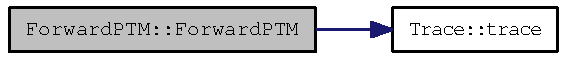
\includegraphics[width=154pt]{classForwardPTM_a42913d0481561a489b8664cd22cf7b0c_cgraph}
\end{center}
\end{figure}
\hypertarget{classForwardPTM_a9fa8aa77099a6bb8d4fbe326a5d84704}{
\index{ForwardPTM@{ForwardPTM}!$\sim$ForwardPTM@{$\sim$ForwardPTM}}
\index{$\sim$ForwardPTM@{$\sim$ForwardPTM}!ForwardPTM@{ForwardPTM}}
\subsubsection[{$\sim$ForwardPTM}]{\setlength{\rightskip}{0pt plus 5cm}ForwardPTM::$\sim$ForwardPTM ()}}
\label{classForwardPTM_a9fa8aa77099a6bb8d4fbe326a5d84704}


The documentation for this class was generated from the following files:\begin{DoxyCompactItemize}
\item 
\hyperlink{CustomInteractions_8h}{CustomInteractions.h}\item 
\hyperlink{CustomInteractions_8cpp}{CustomInteractions.cpp}\end{DoxyCompactItemize}

\hypertarget{classInteraction}{
\section{Interaction Class Reference}
\label{classInteraction}\index{Interaction@{Interaction}}
}


{\ttfamily \#include $<$Interaction.h$>$}Inheritance diagram for Interaction:\nopagebreak
\begin{figure}[H]
\begin{center}
\leavevmode
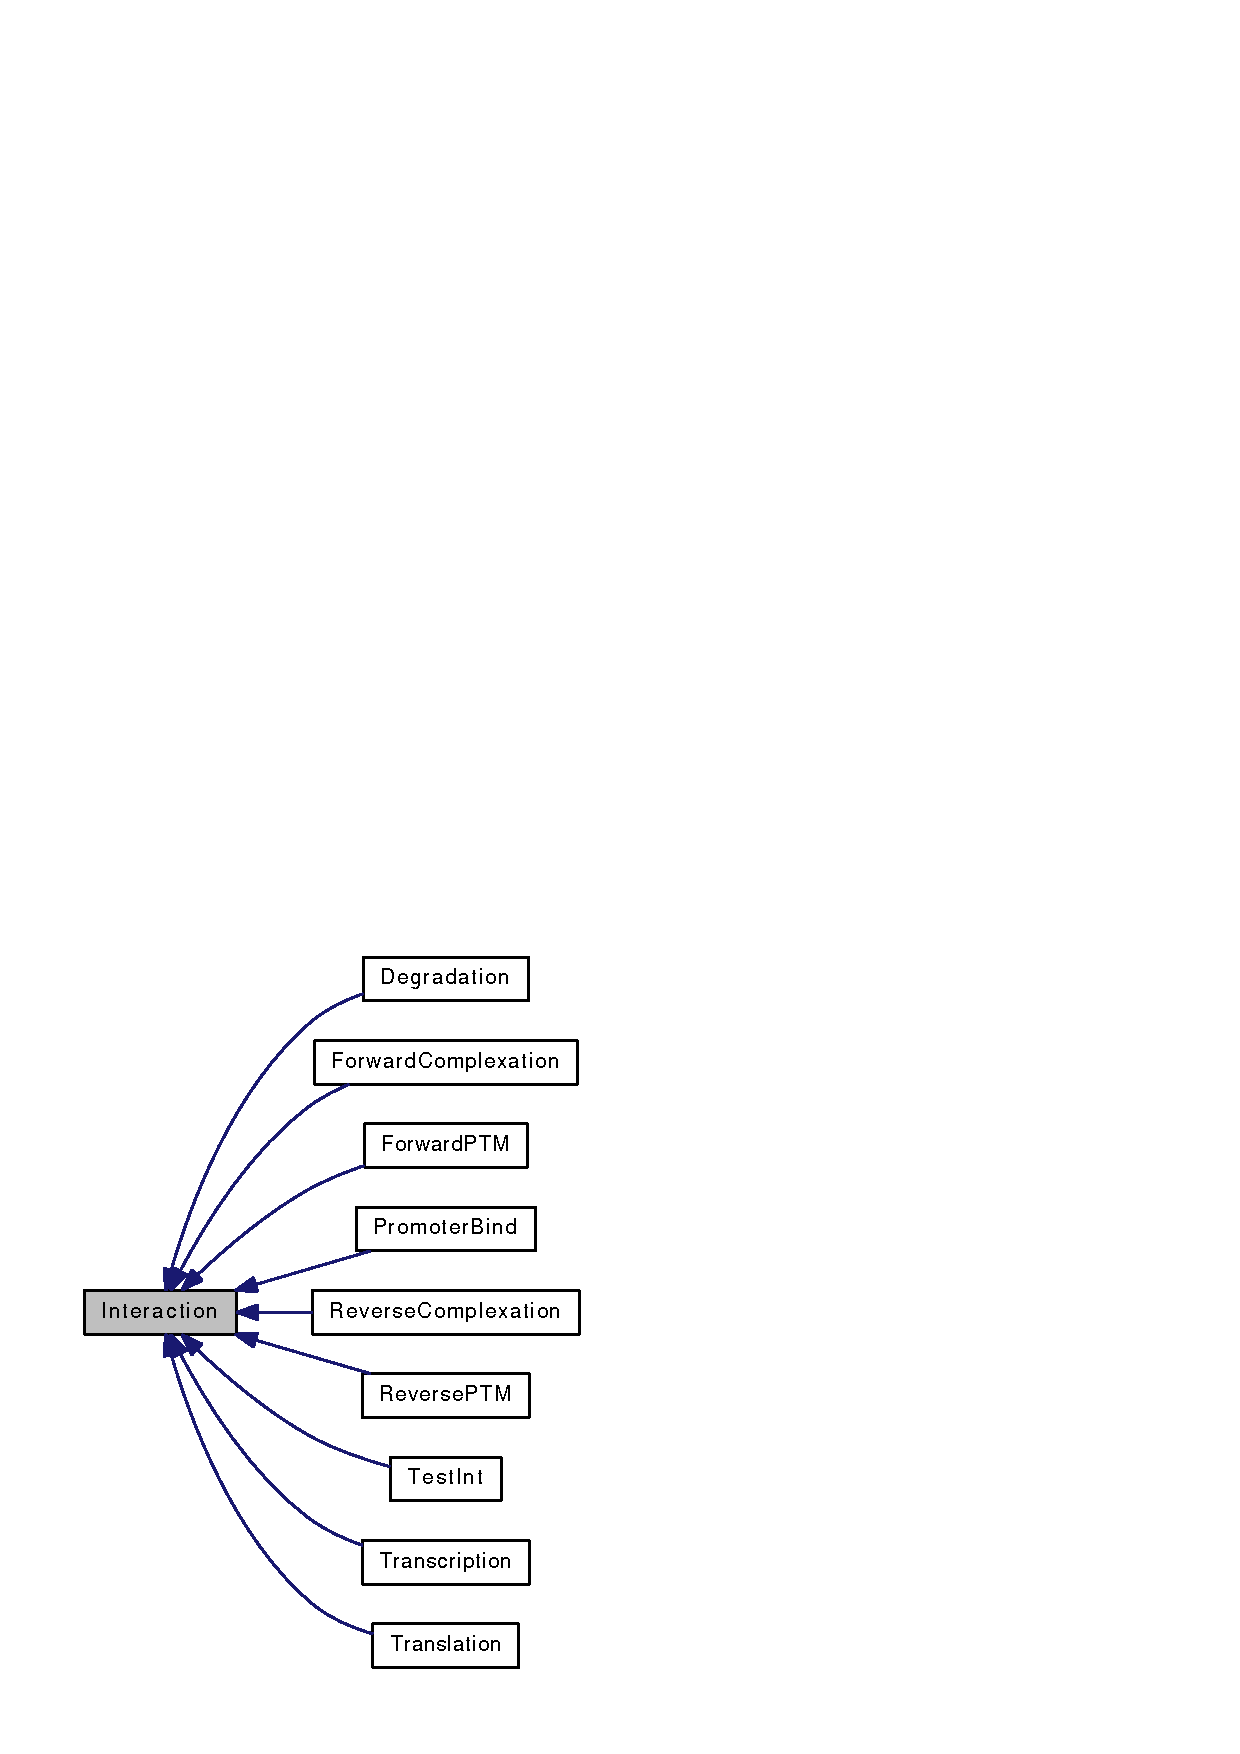
\includegraphics[width=282pt]{classInteraction__inherit__graph}
\end{center}
\end{figure}
\subsection*{Public Member Functions}
\begin{DoxyCompactItemize}
\item 
\hyperlink{classInteraction_aadfd0e254296043c26508d47090ace76}{Interaction} ()
\item 
\hyperlink{classInteraction_a6610199fedc7fae617003cb2f397c825}{$\sim$Interaction} ()
\item 
virtual float \hyperlink{classInteraction_a6328831e714adf9c8177f6052d2e017f}{getEffect} (ListDigraph $\ast$, ListDigraph::NodeMap$<$ \hyperlink{classMolecule}{Molecule} $\ast$ $>$ $\ast$, ListDigraph::ArcMap$<$ \hyperlink{classInteraction}{Interaction} $\ast$ $>$ $\ast$, ListDigraph::Node, int, float)
\item 
const char $\ast$ \hyperlink{classInteraction_a64c55f6b12dca30cc1793c30614220f4}{getName} ()
\item 
float \hyperlink{classInteraction_a82197452596f6bd849df062c5f9d9714}{setRate} (float)
\item 
virtual float \hyperlink{classInteraction_a5ff512276a432b6aa172e719d4866131}{getRate} ()
\end{DoxyCompactItemize}
\subsection*{Public Attributes}
\begin{DoxyCompactItemize}
\item 
const char $\ast$ \hyperlink{classInteraction_a32877e378c8312363a02622d09ae67d4}{name}
\item 
int \hyperlink{classInteraction_a3f30aa82589c3b34bb2feb0b09835aad}{arcID}
\end{DoxyCompactItemize}
\subsection*{Protected Attributes}
\begin{DoxyCompactItemize}
\item 
float \hyperlink{classInteraction_a0a5f4ea012be478c8fe13de552ea5055}{rate}
\end{DoxyCompactItemize}


\subsection{Constructor \& Destructor Documentation}
\hypertarget{classInteraction_aadfd0e254296043c26508d47090ace76}{
\index{Interaction@{Interaction}!Interaction@{Interaction}}
\index{Interaction@{Interaction}!Interaction@{Interaction}}
\subsubsection[{Interaction}]{\setlength{\rightskip}{0pt plus 5cm}Interaction::Interaction ()}}
\label{classInteraction_aadfd0e254296043c26508d47090ace76}
\hyperlink{classInteraction}{Interaction} base class implementation \hyperlink{classInteraction_aadfd0e254296043c26508d47090ace76}{Interaction::Interaction()}

\hyperlink{classInteraction}{Interaction} default constructor. 

Here is the call graph for this function:\nopagebreak
\begin{figure}[H]
\begin{center}
\leavevmode
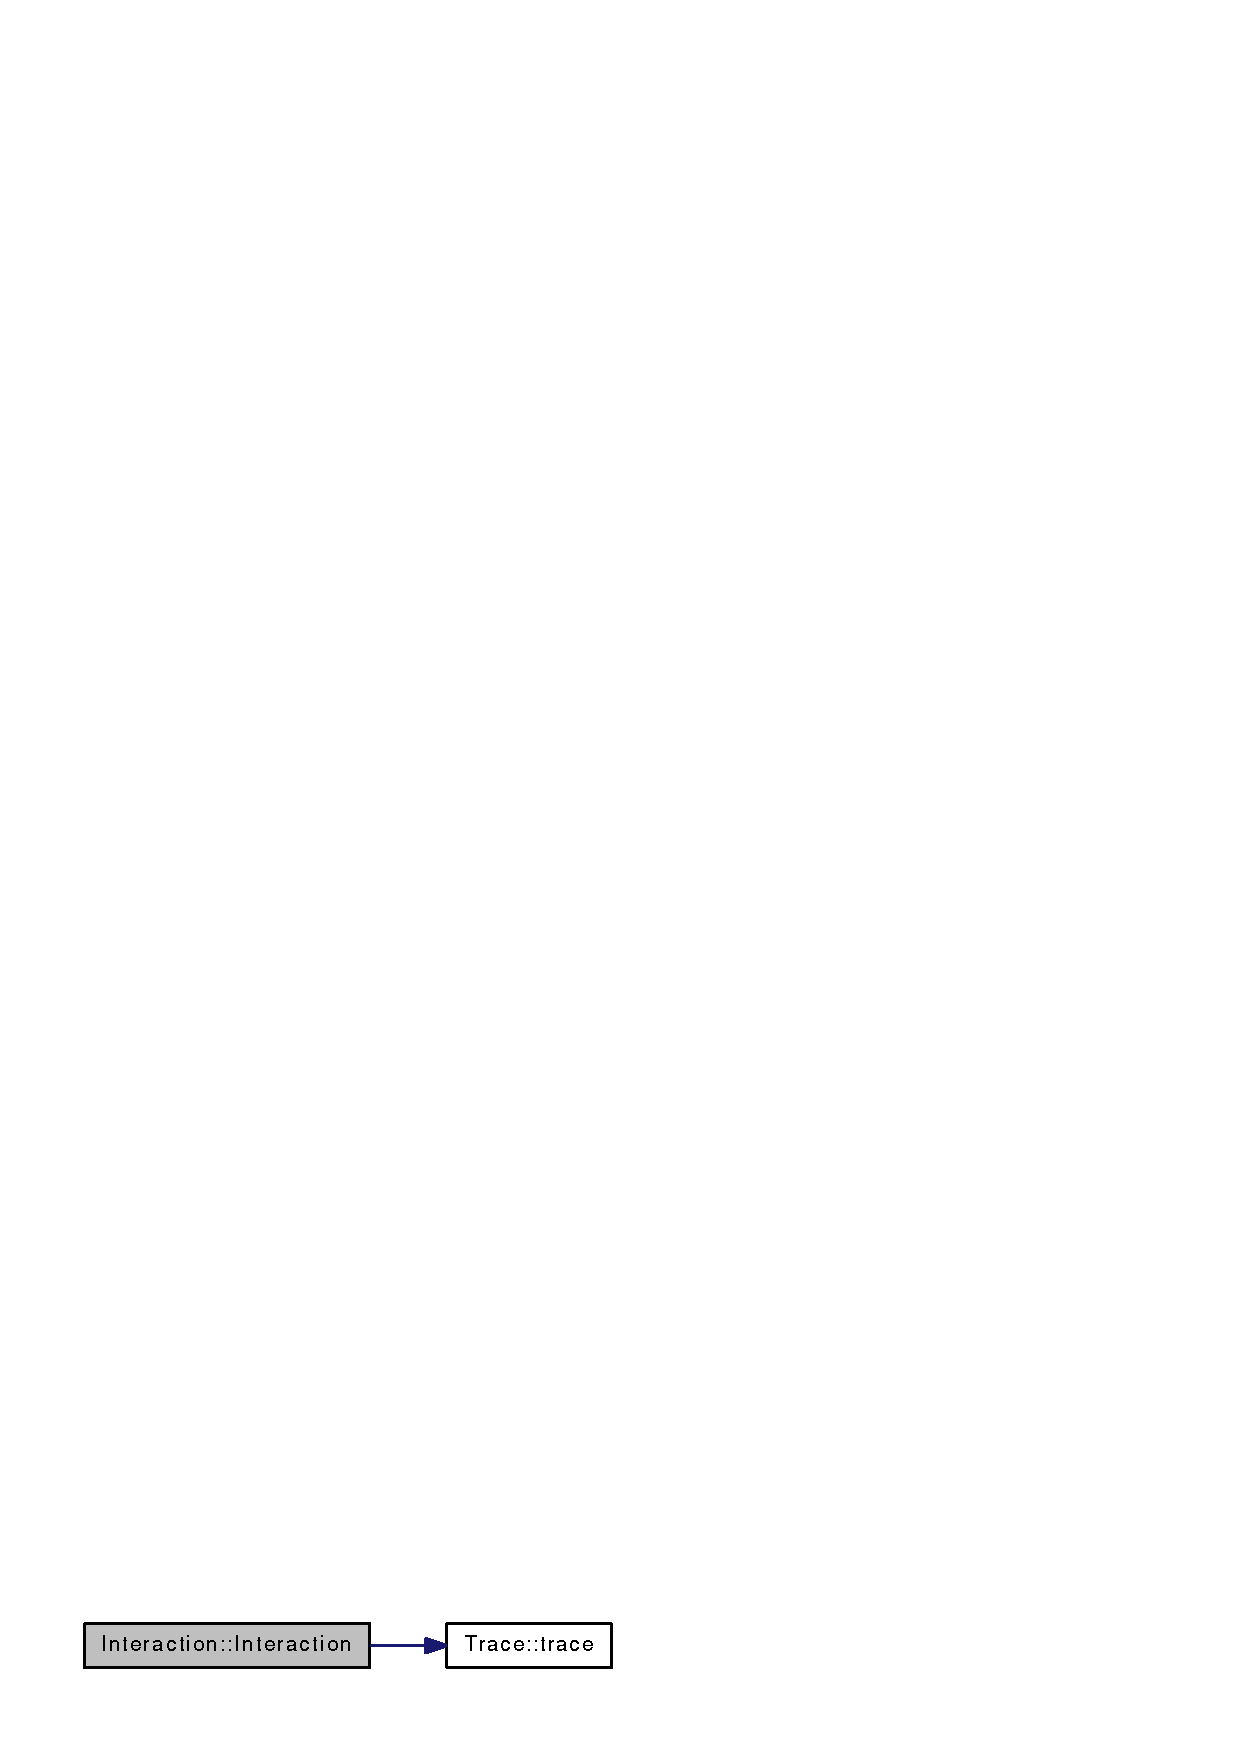
\includegraphics[width=149pt]{classInteraction_aadfd0e254296043c26508d47090ace76_cgraph}
\end{center}
\end{figure}
\hypertarget{classInteraction_a6610199fedc7fae617003cb2f397c825}{
\index{Interaction@{Interaction}!$\sim$Interaction@{$\sim$Interaction}}
\index{$\sim$Interaction@{$\sim$Interaction}!Interaction@{Interaction}}
\subsubsection[{$\sim$Interaction}]{\setlength{\rightskip}{0pt plus 5cm}Interaction::$\sim$Interaction ()}}
\label{classInteraction_a6610199fedc7fae617003cb2f397c825}
\hyperlink{classInteraction_a6610199fedc7fae617003cb2f397c825}{Interaction::$\sim$Interaction()}

\hyperlink{classInteraction}{Interaction} default destructor. 

Here is the call graph for this function:\nopagebreak
\begin{figure}[H]
\begin{center}
\leavevmode
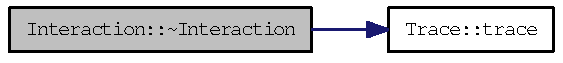
\includegraphics[width=153pt]{classInteraction_a6610199fedc7fae617003cb2f397c825_cgraph}
\end{center}
\end{figure}


\subsection{Member Function Documentation}
\hypertarget{classInteraction_a6328831e714adf9c8177f6052d2e017f}{
\index{Interaction@{Interaction}!getEffect@{getEffect}}
\index{getEffect@{getEffect}!Interaction@{Interaction}}
\subsubsection[{getEffect}]{\setlength{\rightskip}{0pt plus 5cm}float Interaction::getEffect (ListDigraph $\ast$ {\em g}, \/  ListDigraph::NodeMap$<$ {\bf Molecule} $\ast$ $>$ $\ast$ {\em m}, \/  ListDigraph::ArcMap$<$ {\bf Interaction} $\ast$ $>$ $\ast$ {\em i}, \/  ListDigraph::Node {\em a}, \/  int {\em rkIter}, \/  float {\em rkStep})\hspace{0.3cm}{\ttfamily  \mbox{[}virtual\mbox{]}}}}
\label{classInteraction_a6328831e714adf9c8177f6052d2e017f}
float Interaction::getEffect(ListDigraph$\ast$ , NodeMap$<$Molecule$\ast$$>$$\ast$ , ArcMap$<$Interaction$\ast$$>$$\ast$ , Node , int, float)

Get the effect this interaction has on a particular node.

This method defines the behavior of an interaction which connects two molecules. The effect on Node a can be dependent on any other molecule, which can be accessed using the ListDigraph, NodeMap, and ArcMap parameters.

Runge-\/Kutta iteratively approximates the change in concentration during a given timestep. The first iteration is based soley on the current concentration, and each further iteration takes the result of the previous iteration into account. The Runge-\/Kutta data are stored in each molecule, and it is necessary to call Molecule::rkApprox(stepsize, iteration) rather than \hyperlink{classMolecule_a554ea822918374775d5f52b5d49d8195}{Molecule::getValue()} to get the current Iteration's approximated concentration.


\begin{DoxyParams}{Parameters}
\item[{\em g}]The graph object containing Node-\/Node relationships. \item[{\em m}]The NodeMap object containing Node-\/Molecule mappings. \item[{\em i}]The ArcMap object containing Arc-\/Interaction mappings. \item[{\em a}]The Node to calculate the effect for \item[{\em rkIter}]The current iteration of Runge-\/Kutta \mbox{[}0,3\mbox{]} \item[{\em rkStep}]The stepsize of Runge-\/Kutta \end{DoxyParams}


Reimplemented in \hyperlink{classTestInt_a7e6d8e60a2ebc357052a7776244893d7}{TestInt}, \hyperlink{classTranscription_a73f9e09dac4b601a297fd4d59c92cea5}{Transcription}, \hyperlink{classDegradation_a3cad4fc84026c6f627306a7e35527f3c}{Degradation}, \hyperlink{classTranslation_a6599a0f28a58b5adf122d8b8c6206061}{Translation}, \hyperlink{classForwardComplexation_a8f7f867b98b484ed0f09192ebd280e1a}{ForwardComplexation}, \hyperlink{classReverseComplexation_a9dceec2b67efbe7c14a7e53c959263f5}{ReverseComplexation}, and \hyperlink{classPromoterBind_afadb621f9976cc52d83caec0e8613244}{PromoterBind}.

Here is the call graph for this function:\nopagebreak
\begin{figure}[H]
\begin{center}
\leavevmode
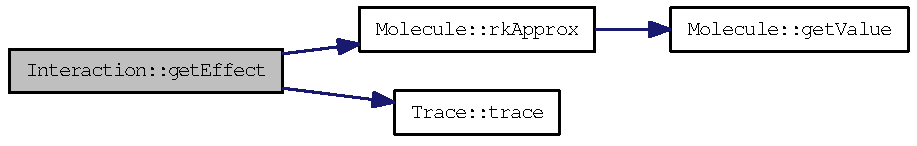
\includegraphics[width=238pt]{classInteraction_a6328831e714adf9c8177f6052d2e017f_cgraph}
\end{center}
\end{figure}
\hypertarget{classInteraction_a64c55f6b12dca30cc1793c30614220f4}{
\index{Interaction@{Interaction}!getName@{getName}}
\index{getName@{getName}!Interaction@{Interaction}}
\subsubsection[{getName}]{\setlength{\rightskip}{0pt plus 5cm}const char $\ast$ Interaction::getName ()}}
\label{classInteraction_a64c55f6b12dca30cc1793c30614220f4}
\hypertarget{classInteraction_a5ff512276a432b6aa172e719d4866131}{
\index{Interaction@{Interaction}!getRate@{getRate}}
\index{getRate@{getRate}!Interaction@{Interaction}}
\subsubsection[{getRate}]{\setlength{\rightskip}{0pt plus 5cm}float Interaction::getRate ()\hspace{0.3cm}{\ttfamily  \mbox{[}virtual\mbox{]}}}}
\label{classInteraction_a5ff512276a432b6aa172e719d4866131}
\hypertarget{classInteraction_a82197452596f6bd849df062c5f9d9714}{
\index{Interaction@{Interaction}!setRate@{setRate}}
\index{setRate@{setRate}!Interaction@{Interaction}}
\subsubsection[{setRate}]{\setlength{\rightskip}{0pt plus 5cm}float Interaction::setRate (float {\em f})}}
\label{classInteraction_a82197452596f6bd849df062c5f9d9714}
void \hyperlink{classInteraction_a82197452596f6bd849df062c5f9d9714}{Interaction::setRate(float)}

Change the kinetic rate of the \hyperlink{classInteraction}{Interaction}


\begin{DoxyParams}{Parameters}
\item[{\em f}]the new rate for the interaction\end{DoxyParams}
\begin{DoxyReturn}{Returns}
the old rate for the interaction 
\end{DoxyReturn}


\subsection{Member Data Documentation}
\hypertarget{classInteraction_a3f30aa82589c3b34bb2feb0b09835aad}{
\index{Interaction@{Interaction}!arcID@{arcID}}
\index{arcID@{arcID}!Interaction@{Interaction}}
\subsubsection[{arcID}]{\setlength{\rightskip}{0pt plus 5cm}int {\bf Interaction::arcID}}}
\label{classInteraction_a3f30aa82589c3b34bb2feb0b09835aad}
\hypertarget{classInteraction_a32877e378c8312363a02622d09ae67d4}{
\index{Interaction@{Interaction}!name@{name}}
\index{name@{name}!Interaction@{Interaction}}
\subsubsection[{name}]{\setlength{\rightskip}{0pt plus 5cm}const char$\ast$ {\bf Interaction::name}}}
\label{classInteraction_a32877e378c8312363a02622d09ae67d4}
\hypertarget{classInteraction_a0a5f4ea012be478c8fe13de552ea5055}{
\index{Interaction@{Interaction}!rate@{rate}}
\index{rate@{rate}!Interaction@{Interaction}}
\subsubsection[{rate}]{\setlength{\rightskip}{0pt plus 5cm}float {\bf Interaction::rate}\hspace{0.3cm}{\ttfamily  \mbox{[}protected\mbox{]}}}}
\label{classInteraction_a0a5f4ea012be478c8fe13de552ea5055}


The documentation for this class was generated from the following files:\begin{DoxyCompactItemize}
\item 
\hyperlink{Interaction_8h}{Interaction.h}\item 
\hyperlink{Interaction_8cpp}{Interaction.cpp}\end{DoxyCompactItemize}

\hypertarget{classMolecule}{
\section{Molecule Class Reference}
\label{classMolecule}\index{Molecule@{Molecule}}
}


{\ttfamily \#include $<$Molecule.h$>$}Inheritance diagram for Molecule:\nopagebreak
\begin{figure}[H]
\begin{center}
\leavevmode
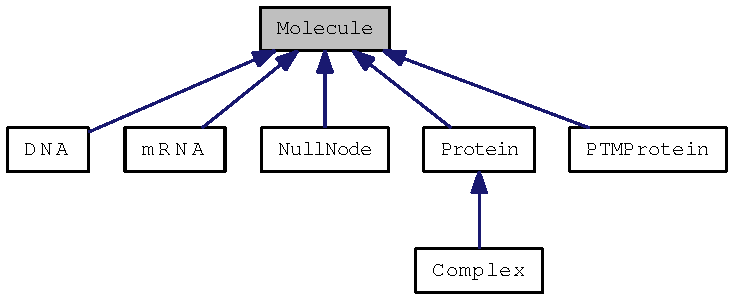
\includegraphics[width=388pt]{classMolecule__inherit__graph}
\end{center}
\end{figure}
\subsection*{Public Member Functions}
\begin{DoxyCompactItemize}
\item 
\hyperlink{classMolecule_a7e7d290ae641518ad4c4d5303b519d0f}{Molecule} ()
\item 
virtual \hyperlink{classMolecule_a1ff980b574a62526abff3d631c83bf94}{$\sim$Molecule} ()
\item 
virtual float \hyperlink{classMolecule_a554ea822918374775d5f52b5d49d8195}{getValue} ()
\item 
void \hyperlink{classMolecule_ab1dd1cb050ddb53a5ce4d9635e3ae03b}{updateRkVal} (int, float)
\item 
void \hyperlink{classMolecule_af67c8a4dcbde3f500509ee1bd94ff4ef}{nextPoint} (float)
\item 
void \hyperlink{classMolecule_a227fedba365853cee63c4e18669a56fa}{setValue} (float)
\item 
void \hyperlink{classMolecule_ac6c78f4a49e270815d7e7dba311b7e14}{outputRK} ()
\item 
float \hyperlink{classMolecule_a66d5e242462b12c0a742fedec0a6bf78}{getrkVal} (int)
\item 
vector$<$ float $>$ $\ast$ \hyperlink{classMolecule_a4405c3a17adfed340826d8b31e4da589}{getRungeKuttaSolution} ()
\item 
virtual float \hyperlink{classMolecule_adabb58a65655a7f55dae0d82b65d04ba}{rkApprox} (int, float)
\item 
virtual char $\ast$ \hyperlink{classMolecule_a6d8720e89d81c1297beced997ad62718}{getShortName} ()
\item 
virtual char $\ast$ \hyperlink{classMolecule_a6d3c3fd4827a62dacfd9d7a7d3a7f6ea}{getLongName} ()
\item 
void \hyperlink{classMolecule_a4f1f48fc2b13b96d7f8015394895e240}{setID} (int)
\item 
int \hyperlink{classMolecule_a9a596dbbdced6d8cec10ad158d4a9f2a}{getID} ()
\item 
void \hyperlink{classMolecule_ab073ddc977c06fe8f70b2c5108eead8c}{reset} ()
\item 
int \hyperlink{classMolecule_a125243e73faff1e5e482e65ba923ca3a}{getScore} ()
\item 
int \hyperlink{classMolecule_ae946ae8bea91c5893ad9bf0fb66b6e0d}{getPTMCount} (int, int)
\item 
virtual int \hyperlink{classMolecule_a7a8b15817d1f1baafe07b50c29cbbc9d}{getPTMCount} (int)
\end{DoxyCompactItemize}
\subsection*{Public Attributes}
\begin{DoxyCompactItemize}
\item 
int \hyperlink{classMolecule_a4eafa2831869e116f64c86987f1cac81}{nodeID}
\item 
int \hyperlink{classMolecule_a134dd5ffa71953792912c7b0cca01405}{wasPTM}
\item 
int \hyperlink{classMolecule_ae6aff39305dd77531ea5a213b6f2b1c5}{PTMArray} \mbox{[}4\mbox{]}
\item 
MTRand \hyperlink{classMolecule_af036bbaa1f3ec537d3711ae3242d3074}{r}
\end{DoxyCompactItemize}
\subsection*{Protected Attributes}
\begin{DoxyCompactItemize}
\item 
float \hyperlink{classMolecule_ac3b04a11e12391be3fdac1251f0a62d0}{initialConcentration}
\item 
float \hyperlink{classMolecule_a2c7587932c7eae82adedfd1022eefea9}{currentConcentration}
\item 
float \hyperlink{classMolecule_a36d750dfda76602691edfb988f6aee42}{rkVal} \mbox{[}4\mbox{]}
\item 
int \hyperlink{classMolecule_a526a58eb943156887bb75b24bdb2b8a0}{numChanges}
\item 
int \hyperlink{classMolecule_acefb24656feeb161148e9594db6ada0b}{prevDir}
\item 
int \hyperlink{classMolecule_a4cd5591c0a8c07ceec922c4f2e8f295c}{currentDir}
\item 
char \hyperlink{classMolecule_a5b6f24dea7138830541e938e2eed707a}{buf} \mbox{[}200\mbox{]}
\item 
const char $\ast$ \hyperlink{classMolecule_a4ac09eefeba07dcb455014acc1ad00c9}{longName}
\item 
const char $\ast$ \hyperlink{classMolecule_ae79f60ef35ffcb500e91013f59563e03}{shortName}
\item 
int \hyperlink{classMolecule_a563a9a295191833b51660f77749e3628}{moleculeID}
\item 
vector$<$ float $>$ \hyperlink{classMolecule_a3e3be6cd7b1286e8d8d489642ab19641}{rungeKuttaSolution}
\end{DoxyCompactItemize}


\subsection{Constructor \& Destructor Documentation}
\hypertarget{classMolecule_a7e7d290ae641518ad4c4d5303b519d0f}{
\index{Molecule@{Molecule}!Molecule@{Molecule}}
\index{Molecule@{Molecule}!Molecule@{Molecule}}
\subsubsection[{Molecule}]{\setlength{\rightskip}{0pt plus 5cm}Molecule::Molecule ()}}
\label{classMolecule_a7e7d290ae641518ad4c4d5303b519d0f}
\hyperlink{classMolecule_a7e7d290ae641518ad4c4d5303b519d0f}{Molecule::Molecule()}

Default Constructor 

Here is the call graph for this function:\nopagebreak
\begin{figure}[H]
\begin{center}
\leavevmode
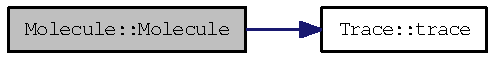
\includegraphics[width=137pt]{classMolecule_a7e7d290ae641518ad4c4d5303b519d0f_cgraph}
\end{center}
\end{figure}
\hypertarget{classMolecule_a1ff980b574a62526abff3d631c83bf94}{
\index{Molecule@{Molecule}!$\sim$Molecule@{$\sim$Molecule}}
\index{$\sim$Molecule@{$\sim$Molecule}!Molecule@{Molecule}}
\subsubsection[{$\sim$Molecule}]{\setlength{\rightskip}{0pt plus 5cm}Molecule::$\sim$Molecule ()\hspace{0.3cm}{\ttfamily  \mbox{[}virtual\mbox{]}}}}
\label{classMolecule_a1ff980b574a62526abff3d631c83bf94}
\hyperlink{classMolecule_a1ff980b574a62526abff3d631c83bf94}{Molecule::$\sim$Molecule()}

Default Destructor 

\subsection{Member Function Documentation}
\hypertarget{classMolecule_a9a596dbbdced6d8cec10ad158d4a9f2a}{
\index{Molecule@{Molecule}!getID@{getID}}
\index{getID@{getID}!Molecule@{Molecule}}
\subsubsection[{getID}]{\setlength{\rightskip}{0pt plus 5cm}int Molecule::getID ()}}
\label{classMolecule_a9a596dbbdced6d8cec10ad158d4a9f2a}
int \hyperlink{classMolecule_a9a596dbbdced6d8cec10ad158d4a9f2a}{Molecule::getID()}

Get the ID of the current molecule.

\begin{DoxyReturn}{Returns}
the current Molecule's ID 
\end{DoxyReturn}
\hypertarget{classMolecule_a6d3c3fd4827a62dacfd9d7a7d3a7f6ea}{
\index{Molecule@{Molecule}!getLongName@{getLongName}}
\index{getLongName@{getLongName}!Molecule@{Molecule}}
\subsubsection[{getLongName}]{\setlength{\rightskip}{0pt plus 5cm}char $\ast$ Molecule::getLongName ()\hspace{0.3cm}{\ttfamily  \mbox{[}virtual\mbox{]}}}}
\label{classMolecule_a6d3c3fd4827a62dacfd9d7a7d3a7f6ea}
char$\ast$ \hyperlink{classMolecule_a6d3c3fd4827a62dacfd9d7a7d3a7f6ea}{Molecule::getLongName()} (Virtual function)

Return the \char`\"{}long\char`\"{} name of a molecule.

The long name consists of the long prefix set in the constructor appended to the moleculeID with a space in between. Ex. \hyperlink{classDNA}{DNA} 1, \hyperlink{classProtein}{Protein} 3, \hyperlink{classComplex}{Complex} 8

\begin{DoxyReturn}{Returns}
the long name of the current molecule 
\end{DoxyReturn}


Reimplemented in \hyperlink{classPTMProtein_a933492fe6252149290b4a2e9885588da}{PTMProtein}.\hypertarget{classMolecule_a7a8b15817d1f1baafe07b50c29cbbc9d}{
\index{Molecule@{Molecule}!getPTMCount@{getPTMCount}}
\index{getPTMCount@{getPTMCount}!Molecule@{Molecule}}
\subsubsection[{getPTMCount}]{\setlength{\rightskip}{0pt plus 5cm}int Molecule::getPTMCount (int {\em index})\hspace{0.3cm}{\ttfamily  \mbox{[}virtual\mbox{]}}}}
\label{classMolecule_a7a8b15817d1f1baafe07b50c29cbbc9d}
\hypertarget{classMolecule_ae946ae8bea91c5893ad9bf0fb66b6e0d}{
\index{Molecule@{Molecule}!getPTMCount@{getPTMCount}}
\index{getPTMCount@{getPTMCount}!Molecule@{Molecule}}
\subsubsection[{getPTMCount}]{\setlength{\rightskip}{0pt plus 5cm}int Molecule::getPTMCount (int, \/  int)}}
\label{classMolecule_ae946ae8bea91c5893ad9bf0fb66b6e0d}
\hypertarget{classMolecule_a66d5e242462b12c0a742fedec0a6bf78}{
\index{Molecule@{Molecule}!getrkVal@{getrkVal}}
\index{getrkVal@{getrkVal}!Molecule@{Molecule}}
\subsubsection[{getrkVal}]{\setlength{\rightskip}{0pt plus 5cm}float Molecule::getrkVal (int {\em k})}}
\label{classMolecule_a66d5e242462b12c0a742fedec0a6bf78}
float \hyperlink{classMolecule_a66d5e242462b12c0a742fedec0a6bf78}{Molecule::getrkVal(int)}

Get the value of the intermediate Runge-\/Kutta value for a particular iteration.


\begin{DoxyParams}{Parameters}
\item[{\em k}]Which iterations rkVal to return\end{DoxyParams}
\begin{DoxyReturn}{Returns}
The value of this molecules rkVal\mbox{[}k\mbox{]} 
\end{DoxyReturn}
\hypertarget{classMolecule_a4405c3a17adfed340826d8b31e4da589}{
\index{Molecule@{Molecule}!getRungeKuttaSolution@{getRungeKuttaSolution}}
\index{getRungeKuttaSolution@{getRungeKuttaSolution}!Molecule@{Molecule}}
\subsubsection[{getRungeKuttaSolution}]{\setlength{\rightskip}{0pt plus 5cm}vector$<$ float $>$ $\ast$ Molecule::getRungeKuttaSolution ()}}
\label{classMolecule_a4405c3a17adfed340826d8b31e4da589}
\hypertarget{classMolecule_a125243e73faff1e5e482e65ba923ca3a}{
\index{Molecule@{Molecule}!getScore@{getScore}}
\index{getScore@{getScore}!Molecule@{Molecule}}
\subsubsection[{getScore}]{\setlength{\rightskip}{0pt plus 5cm}int Molecule::getScore ()}}
\label{classMolecule_a125243e73faff1e5e482e65ba923ca3a}
\hypertarget{classMolecule_a6d8720e89d81c1297beced997ad62718}{
\index{Molecule@{Molecule}!getShortName@{getShortName}}
\index{getShortName@{getShortName}!Molecule@{Molecule}}
\subsubsection[{getShortName}]{\setlength{\rightskip}{0pt plus 5cm}char $\ast$ Molecule::getShortName ()\hspace{0.3cm}{\ttfamily  \mbox{[}virtual\mbox{]}}}}
\label{classMolecule_a6d8720e89d81c1297beced997ad62718}
char$\ast$ \hyperlink{classMolecule_a6d8720e89d81c1297beced997ad62718}{Molecule::getShortName()} (Virtual function)

Return the \char`\"{}short\char`\"{} name of a molecule.

The short name consists of the short prefix set in the constructor appended to the moleculeID with no space in between. Ex. g1, p4, ptm2

\begin{DoxyReturn}{Returns}
the short name of the current molecule 
\end{DoxyReturn}
\hypertarget{classMolecule_a554ea822918374775d5f52b5d49d8195}{
\index{Molecule@{Molecule}!getValue@{getValue}}
\index{getValue@{getValue}!Molecule@{Molecule}}
\subsubsection[{getValue}]{\setlength{\rightskip}{0pt plus 5cm}float Molecule::getValue ()\hspace{0.3cm}{\ttfamily  \mbox{[}virtual\mbox{]}}}}
\label{classMolecule_a554ea822918374775d5f52b5d49d8195}
float \hyperlink{classMolecule_a554ea822918374775d5f52b5d49d8195}{Molecule::getValue()} (Virtual Function)

Get the current value of this molecule.

\begin{DoxyReturn}{Returns}
the current value of the concentration 
\end{DoxyReturn}


Reimplemented in \hyperlink{classDNA_ac3f4ef00894483313ea44df6a85b3bab}{DNA}, and \hyperlink{classNullNode_ae1cddbf915028ab4f2aebf6879c6a682}{NullNode}.\hypertarget{classMolecule_af67c8a4dcbde3f500509ee1bd94ff4ef}{
\index{Molecule@{Molecule}!nextPoint@{nextPoint}}
\index{nextPoint@{nextPoint}!Molecule@{Molecule}}
\subsubsection[{nextPoint}]{\setlength{\rightskip}{0pt plus 5cm}void Molecule::nextPoint (float {\em step})}}
\label{classMolecule_af67c8a4dcbde3f500509ee1bd94ff4ef}
void \hyperlink{classMolecule_af67c8a4dcbde3f500509ee1bd94ff4ef}{Molecule::nextPoint(float)}

Adds a data point to the rungeKuttaSolution based on the rkVals calculated by Runge-\/Kutta


\begin{DoxyParams}{Parameters}
\item[{\em step}]The stepsize used to calculate the rkVals \end{DoxyParams}


Here is the call graph for this function:\nopagebreak
\begin{figure}[H]
\begin{center}
\leavevmode
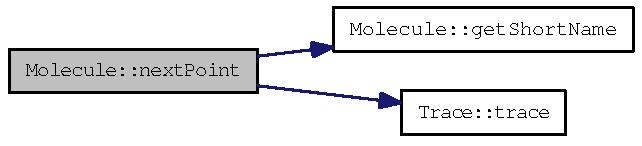
\includegraphics[width=172pt]{classMolecule_af67c8a4dcbde3f500509ee1bd94ff4ef_cgraph}
\end{center}
\end{figure}
\hypertarget{classMolecule_ac6c78f4a49e270815d7e7dba311b7e14}{
\index{Molecule@{Molecule}!outputRK@{outputRK}}
\index{outputRK@{outputRK}!Molecule@{Molecule}}
\subsubsection[{outputRK}]{\setlength{\rightskip}{0pt plus 5cm}void Molecule::outputRK ()}}
\label{classMolecule_ac6c78f4a49e270815d7e7dba311b7e14}
void \hyperlink{classMolecule_ac6c78f4a49e270815d7e7dba311b7e14}{Molecule::outputRK()}

TEST METHOD 

Here is the call graph for this function:\nopagebreak
\begin{figure}[H]
\begin{center}
\leavevmode
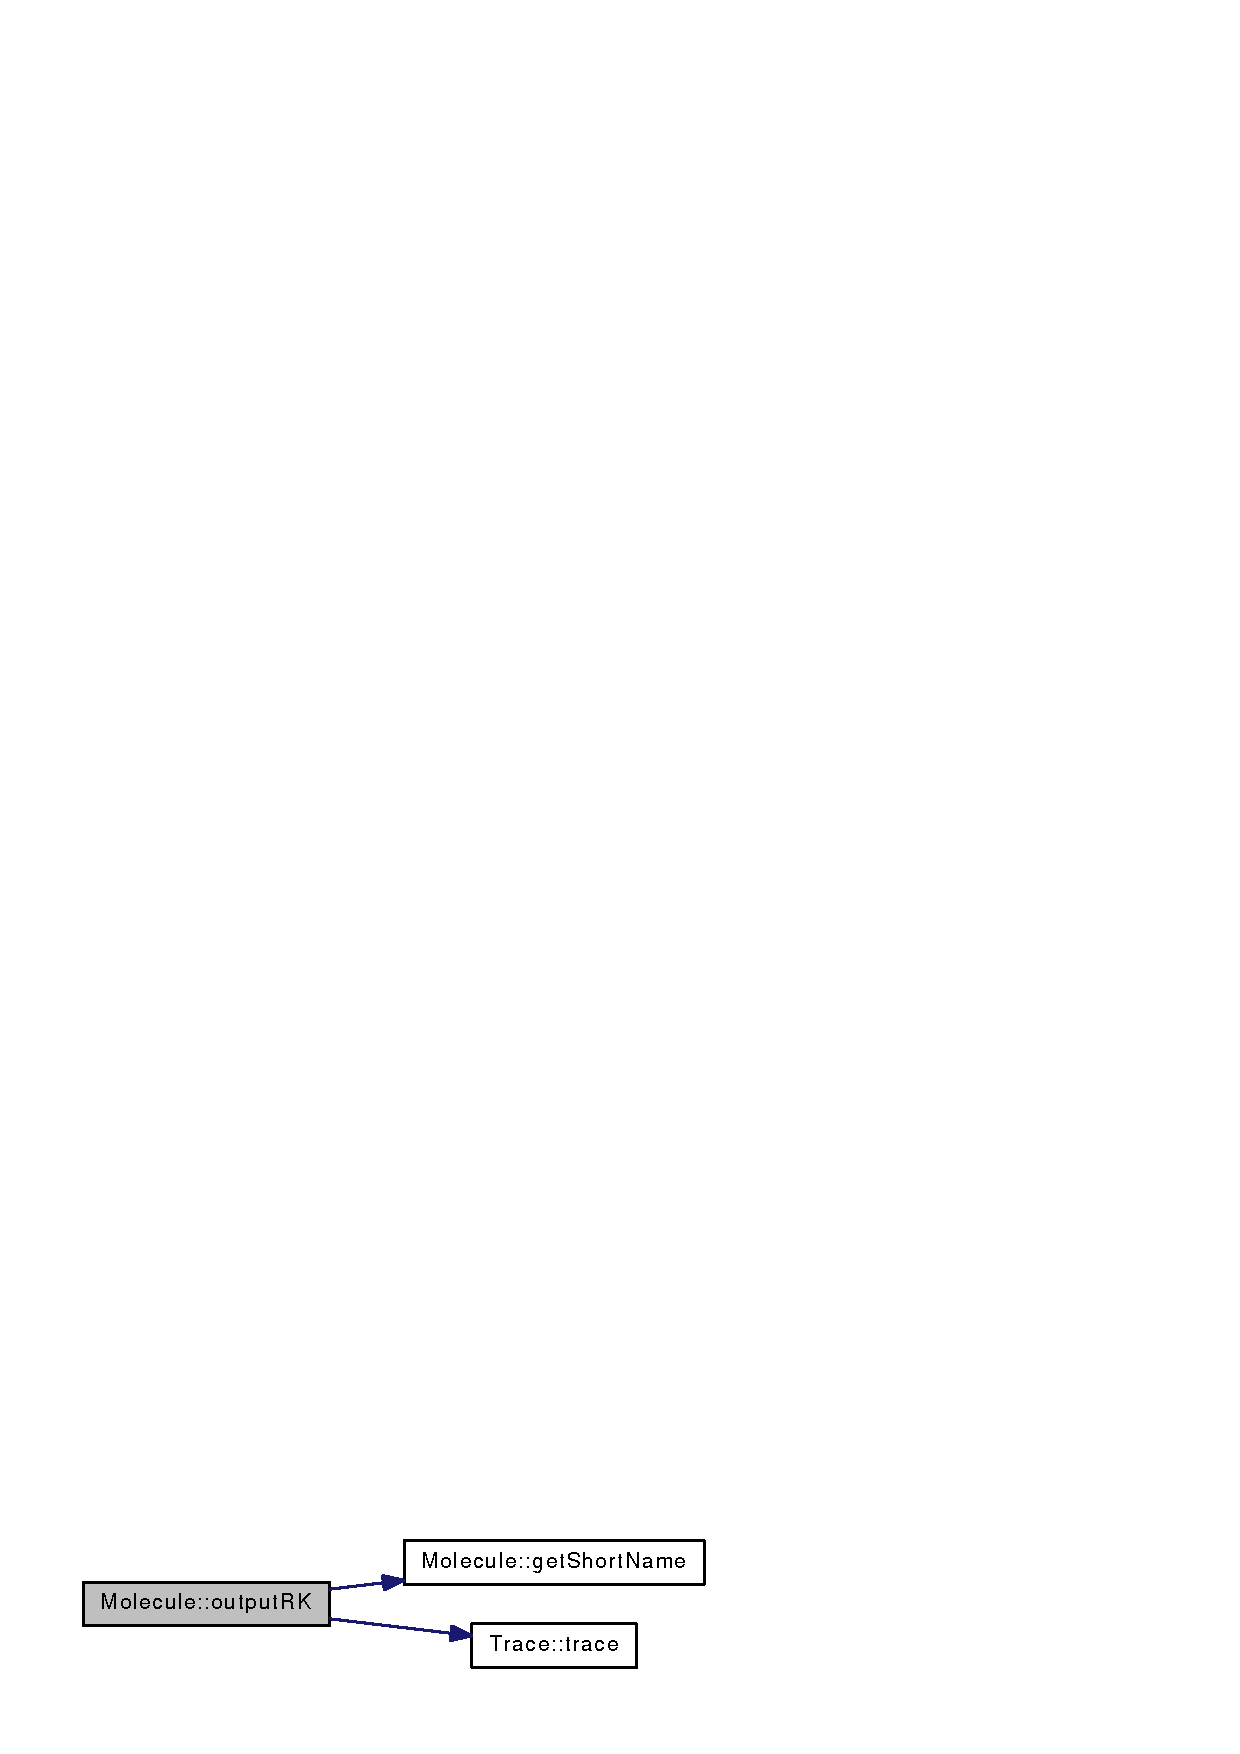
\includegraphics[width=171pt]{classMolecule_ac6c78f4a49e270815d7e7dba311b7e14_cgraph}
\end{center}
\end{figure}
\hypertarget{classMolecule_ab073ddc977c06fe8f70b2c5108eead8c}{
\index{Molecule@{Molecule}!reset@{reset}}
\index{reset@{reset}!Molecule@{Molecule}}
\subsubsection[{reset}]{\setlength{\rightskip}{0pt plus 5cm}void Molecule::reset ()}}
\label{classMolecule_ab073ddc977c06fe8f70b2c5108eead8c}
void \hyperlink{classMolecule_ab073ddc977c06fe8f70b2c5108eead8c}{Molecule::reset()}

Reset the molecule between Runge-\/Kutta runs. The vector containing runge-\/kutta data points is erased, the initial concentration is added as the first element, and the rkVals are all reset to 0. \hypertarget{classMolecule_adabb58a65655a7f55dae0d82b65d04ba}{
\index{Molecule@{Molecule}!rkApprox@{rkApprox}}
\index{rkApprox@{rkApprox}!Molecule@{Molecule}}
\subsubsection[{rkApprox}]{\setlength{\rightskip}{0pt plus 5cm}float Molecule::rkApprox (int {\em rkIteration}, \/  float {\em rkStepSize})\hspace{0.3cm}{\ttfamily  \mbox{[}virtual\mbox{]}}}}
\label{classMolecule_adabb58a65655a7f55dae0d82b65d04ba}
float \hyperlink{classMolecule_adabb58a65655a7f55dae0d82b65d04ba}{Molecule::rkApprox(int, float)} (Virtual Function)

Returns the next approximate value of this molecule for the next timestep for the specified stage of Runge-\/Kutta. Runge-\/Kutta uses successive iterations to make more accurate approximations of a solution.

rkApprox should be used in \hyperlink{classInteraction_a6328831e714adf9c8177f6052d2e017f}{Interaction::getEffect}, to provide the Runge-\/Kutta corrected concentrations of molecules during runge-\/kutta calculation instead of the base value for all iterations.


\begin{DoxyParams}{Parameters}
\item[{\em rkIteration}]the current iteration of Runge-\/Kutta \item[{\em rkStepSize}]the timestep being used by Runge-\/Kutta \end{DoxyParams}


Reimplemented in \hyperlink{classDNA_a10bec8cdc5922b2780887666c53891f1}{DNA}.

Here is the call graph for this function:\nopagebreak
\begin{figure}[H]
\begin{center}
\leavevmode
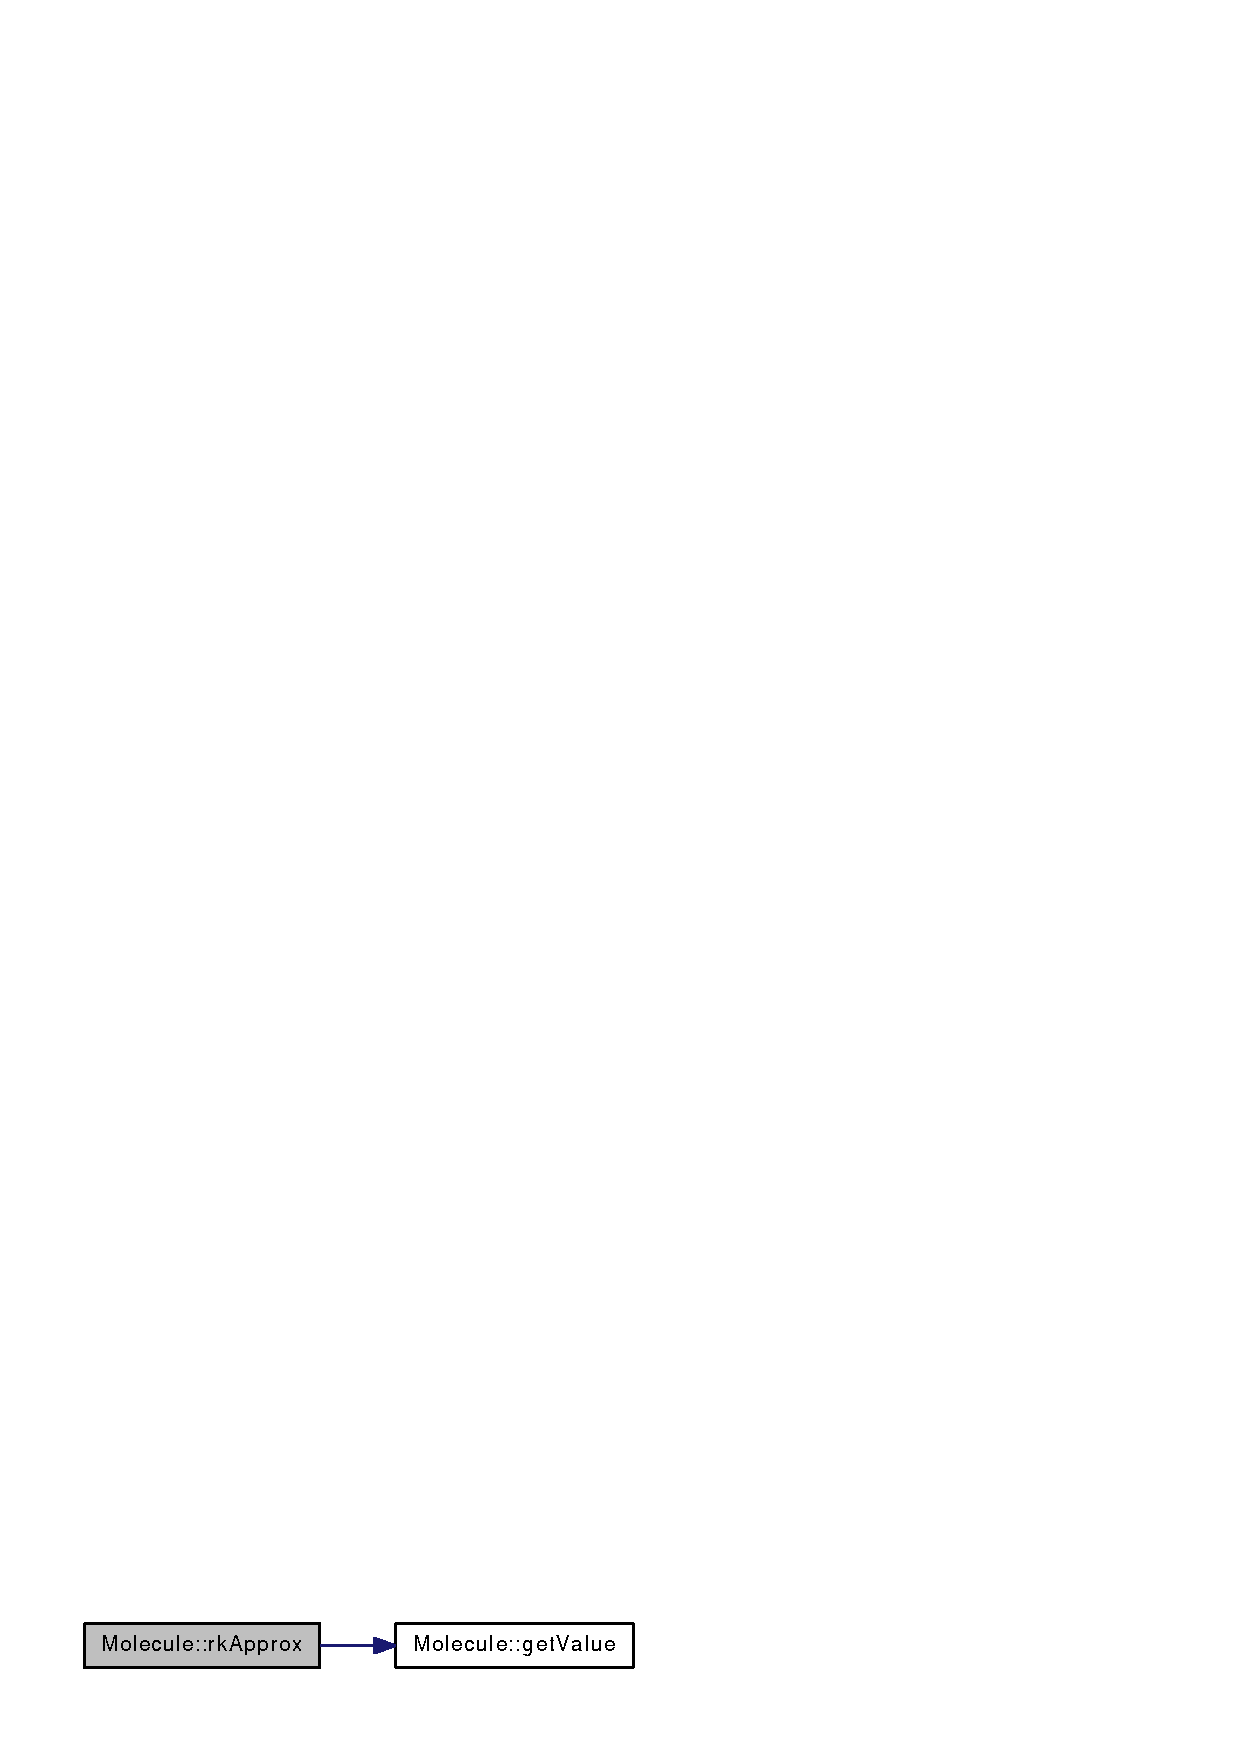
\includegraphics[width=154pt]{classMolecule_adabb58a65655a7f55dae0d82b65d04ba_cgraph}
\end{center}
\end{figure}
\hypertarget{classMolecule_a4f1f48fc2b13b96d7f8015394895e240}{
\index{Molecule@{Molecule}!setID@{setID}}
\index{setID@{setID}!Molecule@{Molecule}}
\subsubsection[{setID}]{\setlength{\rightskip}{0pt plus 5cm}void Molecule::setID (int {\em i})}}
\label{classMolecule_a4f1f48fc2b13b96d7f8015394895e240}
void \hyperlink{classMolecule_a4f1f48fc2b13b96d7f8015394895e240}{Molecule::setID(int)}

Set the ID of a molecule, used when displaying molecule names. The ID is a number which is not necessarily unique, but should only be shared between strongly related molecules. \hypertarget{classMolecule_a227fedba365853cee63c4e18669a56fa}{
\index{Molecule@{Molecule}!setValue@{setValue}}
\index{setValue@{setValue}!Molecule@{Molecule}}
\subsubsection[{setValue}]{\setlength{\rightskip}{0pt plus 5cm}void Molecule::setValue (float {\em v})}}
\label{classMolecule_a227fedba365853cee63c4e18669a56fa}
void \hyperlink{classMolecule_a227fedba365853cee63c4e18669a56fa}{Molecule::setValue(float)}


\begin{DoxyParams}{Parameters}
\item[{\em v}]the new value to set as the concentration \end{DoxyParams}
\hypertarget{classMolecule_ab1dd1cb050ddb53a5ce4d9635e3ae03b}{
\index{Molecule@{Molecule}!updateRkVal@{updateRkVal}}
\index{updateRkVal@{updateRkVal}!Molecule@{Molecule}}
\subsubsection[{updateRkVal}]{\setlength{\rightskip}{0pt plus 5cm}void Molecule::updateRkVal (int {\em index}, \/  float {\em amount})}}
\label{classMolecule_ab1dd1cb050ddb53a5ce4d9635e3ae03b}
void \hyperlink{classMolecule_ab1dd1cb050ddb53a5ce4d9635e3ae03b}{Molecule::updateRkVal(int, float)}

Adds some amount to the specified intermediate values used by Runge-\/Kutta.


\begin{DoxyParams}{Parameters}
\item[{\em index}]The index of the rkValue array to update \item[{\em amount}]The amount to add to the rkValue array \end{DoxyParams}


Here is the call graph for this function:\nopagebreak
\begin{figure}[H]
\begin{center}
\leavevmode
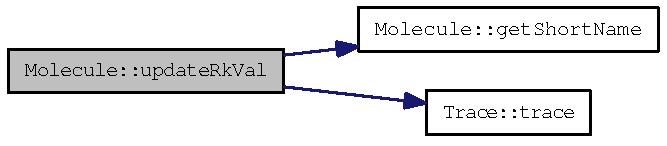
\includegraphics[width=178pt]{classMolecule_ab1dd1cb050ddb53a5ce4d9635e3ae03b_cgraph}
\end{center}
\end{figure}


\subsection{Member Data Documentation}
\hypertarget{classMolecule_a5b6f24dea7138830541e938e2eed707a}{
\index{Molecule@{Molecule}!buf@{buf}}
\index{buf@{buf}!Molecule@{Molecule}}
\subsubsection[{buf}]{\setlength{\rightskip}{0pt plus 5cm}char {\bf Molecule::buf}\mbox{[}200\mbox{]}\hspace{0.3cm}{\ttfamily  \mbox{[}protected\mbox{]}}}}
\label{classMolecule_a5b6f24dea7138830541e938e2eed707a}
\hypertarget{classMolecule_a2c7587932c7eae82adedfd1022eefea9}{
\index{Molecule@{Molecule}!currentConcentration@{currentConcentration}}
\index{currentConcentration@{currentConcentration}!Molecule@{Molecule}}
\subsubsection[{currentConcentration}]{\setlength{\rightskip}{0pt plus 5cm}float {\bf Molecule::currentConcentration}\hspace{0.3cm}{\ttfamily  \mbox{[}protected\mbox{]}}}}
\label{classMolecule_a2c7587932c7eae82adedfd1022eefea9}
\hypertarget{classMolecule_a4cd5591c0a8c07ceec922c4f2e8f295c}{
\index{Molecule@{Molecule}!currentDir@{currentDir}}
\index{currentDir@{currentDir}!Molecule@{Molecule}}
\subsubsection[{currentDir}]{\setlength{\rightskip}{0pt plus 5cm}int {\bf Molecule::currentDir}\hspace{0.3cm}{\ttfamily  \mbox{[}protected\mbox{]}}}}
\label{classMolecule_a4cd5591c0a8c07ceec922c4f2e8f295c}
\hypertarget{classMolecule_ac3b04a11e12391be3fdac1251f0a62d0}{
\index{Molecule@{Molecule}!initialConcentration@{initialConcentration}}
\index{initialConcentration@{initialConcentration}!Molecule@{Molecule}}
\subsubsection[{initialConcentration}]{\setlength{\rightskip}{0pt plus 5cm}float {\bf Molecule::initialConcentration}\hspace{0.3cm}{\ttfamily  \mbox{[}protected\mbox{]}}}}
\label{classMolecule_ac3b04a11e12391be3fdac1251f0a62d0}
\hypertarget{classMolecule_a4ac09eefeba07dcb455014acc1ad00c9}{
\index{Molecule@{Molecule}!longName@{longName}}
\index{longName@{longName}!Molecule@{Molecule}}
\subsubsection[{longName}]{\setlength{\rightskip}{0pt plus 5cm}const char$\ast$ {\bf Molecule::longName}\hspace{0.3cm}{\ttfamily  \mbox{[}protected\mbox{]}}}}
\label{classMolecule_a4ac09eefeba07dcb455014acc1ad00c9}
\hypertarget{classMolecule_a563a9a295191833b51660f77749e3628}{
\index{Molecule@{Molecule}!moleculeID@{moleculeID}}
\index{moleculeID@{moleculeID}!Molecule@{Molecule}}
\subsubsection[{moleculeID}]{\setlength{\rightskip}{0pt plus 5cm}int {\bf Molecule::moleculeID}\hspace{0.3cm}{\ttfamily  \mbox{[}protected\mbox{]}}}}
\label{classMolecule_a563a9a295191833b51660f77749e3628}
\hypertarget{classMolecule_a4eafa2831869e116f64c86987f1cac81}{
\index{Molecule@{Molecule}!nodeID@{nodeID}}
\index{nodeID@{nodeID}!Molecule@{Molecule}}
\subsubsection[{nodeID}]{\setlength{\rightskip}{0pt plus 5cm}int {\bf Molecule::nodeID}}}
\label{classMolecule_a4eafa2831869e116f64c86987f1cac81}
\hypertarget{classMolecule_a526a58eb943156887bb75b24bdb2b8a0}{
\index{Molecule@{Molecule}!numChanges@{numChanges}}
\index{numChanges@{numChanges}!Molecule@{Molecule}}
\subsubsection[{numChanges}]{\setlength{\rightskip}{0pt plus 5cm}int {\bf Molecule::numChanges}\hspace{0.3cm}{\ttfamily  \mbox{[}protected\mbox{]}}}}
\label{classMolecule_a526a58eb943156887bb75b24bdb2b8a0}
\hypertarget{classMolecule_acefb24656feeb161148e9594db6ada0b}{
\index{Molecule@{Molecule}!prevDir@{prevDir}}
\index{prevDir@{prevDir}!Molecule@{Molecule}}
\subsubsection[{prevDir}]{\setlength{\rightskip}{0pt plus 5cm}int {\bf Molecule::prevDir}\hspace{0.3cm}{\ttfamily  \mbox{[}protected\mbox{]}}}}
\label{classMolecule_acefb24656feeb161148e9594db6ada0b}
\hypertarget{classMolecule_ae6aff39305dd77531ea5a213b6f2b1c5}{
\index{Molecule@{Molecule}!PTMArray@{PTMArray}}
\index{PTMArray@{PTMArray}!Molecule@{Molecule}}
\subsubsection[{PTMArray}]{\setlength{\rightskip}{0pt plus 5cm}int {\bf Molecule::PTMArray}\mbox{[}4\mbox{]}}}
\label{classMolecule_ae6aff39305dd77531ea5a213b6f2b1c5}
\hypertarget{classMolecule_af036bbaa1f3ec537d3711ae3242d3074}{
\index{Molecule@{Molecule}!r@{r}}
\index{r@{r}!Molecule@{Molecule}}
\subsubsection[{r}]{\setlength{\rightskip}{0pt plus 5cm}MTRand {\bf Molecule::r}}}
\label{classMolecule_af036bbaa1f3ec537d3711ae3242d3074}
\hypertarget{classMolecule_a36d750dfda76602691edfb988f6aee42}{
\index{Molecule@{Molecule}!rkVal@{rkVal}}
\index{rkVal@{rkVal}!Molecule@{Molecule}}
\subsubsection[{rkVal}]{\setlength{\rightskip}{0pt plus 5cm}float {\bf Molecule::rkVal}\mbox{[}4\mbox{]}\hspace{0.3cm}{\ttfamily  \mbox{[}protected\mbox{]}}}}
\label{classMolecule_a36d750dfda76602691edfb988f6aee42}
\hypertarget{classMolecule_a3e3be6cd7b1286e8d8d489642ab19641}{
\index{Molecule@{Molecule}!rungeKuttaSolution@{rungeKuttaSolution}}
\index{rungeKuttaSolution@{rungeKuttaSolution}!Molecule@{Molecule}}
\subsubsection[{rungeKuttaSolution}]{\setlength{\rightskip}{0pt plus 5cm}vector$<$float$>$ {\bf Molecule::rungeKuttaSolution}\hspace{0.3cm}{\ttfamily  \mbox{[}protected\mbox{]}}}}
\label{classMolecule_a3e3be6cd7b1286e8d8d489642ab19641}
\hypertarget{classMolecule_ae79f60ef35ffcb500e91013f59563e03}{
\index{Molecule@{Molecule}!shortName@{shortName}}
\index{shortName@{shortName}!Molecule@{Molecule}}
\subsubsection[{shortName}]{\setlength{\rightskip}{0pt plus 5cm}const char$\ast$ {\bf Molecule::shortName}\hspace{0.3cm}{\ttfamily  \mbox{[}protected\mbox{]}}}}
\label{classMolecule_ae79f60ef35ffcb500e91013f59563e03}
\hypertarget{classMolecule_a134dd5ffa71953792912c7b0cca01405}{
\index{Molecule@{Molecule}!wasPTM@{wasPTM}}
\index{wasPTM@{wasPTM}!Molecule@{Molecule}}
\subsubsection[{wasPTM}]{\setlength{\rightskip}{0pt plus 5cm}int {\bf Molecule::wasPTM}}}
\label{classMolecule_a134dd5ffa71953792912c7b0cca01405}


The documentation for this class was generated from the following files:\begin{DoxyCompactItemize}
\item 
\hyperlink{Molecule_8h}{Molecule.h}\item 
\hyperlink{Molecule_8cpp}{Molecule.cpp}\end{DoxyCompactItemize}

\hypertarget{classMoleculeType}{
\section{MoleculeType Class Reference}
\label{classMoleculeType}\index{MoleculeType@{MoleculeType}}
}


{\ttfamily \#include $<$MoleculeType.h$>$}\subsection*{Public Member Functions}
\begin{DoxyCompactItemize}
\item 
\hyperlink{classMoleculeType_aac38f7675a0f8a29bd7cecd5e5ddb97b}{MoleculeType} ()
\item 
\hyperlink{classMoleculeType_a1b62655acafa2ba0271a7bc5cab51357}{$\sim$MoleculeType} ()
\end{DoxyCompactItemize}


\subsection{Detailed Description}
\hyperlink{MoleculeType_8h}{MoleculeType.h}

\hyperlink{classMoleculeType}{MoleculeType} holds default information about a type of molecule. 

\subsection{Constructor \& Destructor Documentation}
\hypertarget{classMoleculeType_aac38f7675a0f8a29bd7cecd5e5ddb97b}{
\index{MoleculeType@{MoleculeType}!MoleculeType@{MoleculeType}}
\index{MoleculeType@{MoleculeType}!MoleculeType@{MoleculeType}}
\subsubsection[{MoleculeType}]{\setlength{\rightskip}{0pt plus 5cm}MoleculeType::MoleculeType ()}}
\label{classMoleculeType_aac38f7675a0f8a29bd7cecd5e5ddb97b}
\hypertarget{classMoleculeType_a1b62655acafa2ba0271a7bc5cab51357}{
\index{MoleculeType@{MoleculeType}!$\sim$MoleculeType@{$\sim$MoleculeType}}
\index{$\sim$MoleculeType@{$\sim$MoleculeType}!MoleculeType@{MoleculeType}}
\subsubsection[{$\sim$MoleculeType}]{\setlength{\rightskip}{0pt plus 5cm}MoleculeType::$\sim$MoleculeType ()}}
\label{classMoleculeType_a1b62655acafa2ba0271a7bc5cab51357}


The documentation for this class was generated from the following file:\begin{DoxyCompactItemize}
\item 
\hyperlink{MoleculeType_8h}{MoleculeType.h}\end{DoxyCompactItemize}

\hypertarget{classmRNA}{
\section{mRNA Class Reference}
\label{classmRNA}\index{mRNA@{mRNA}}
}


{\ttfamily \#include $<$CustomMolecules.h$>$}Inheritance diagram for mRNA:\nopagebreak
\begin{figure}[H]
\begin{center}
\leavevmode
\includegraphics[width=106pt]{classmRNA__inherit__graph}
\end{center}
\end{figure}
Collaboration diagram for mRNA:\nopagebreak
\begin{figure}[H]
\begin{center}
\leavevmode
\includegraphics[width=106pt]{classmRNA__coll__graph}
\end{center}
\end{figure}
\subsection*{Public Member Functions}
\begin{DoxyCompactItemize}
\item 
\hyperlink{classmRNA_add6fc6ce355527cdab338afb3c9a118f}{mRNA} ()
\item 
\hyperlink{classmRNA_a31f5c877c9941cee8d9f991c8e40b8ec}{$\sim$mRNA} ()
\end{DoxyCompactItemize}


\subsection{Constructor \& Destructor Documentation}
\hypertarget{classmRNA_add6fc6ce355527cdab338afb3c9a118f}{
\index{mRNA@{mRNA}!mRNA@{mRNA}}
\index{mRNA@{mRNA}!mRNA@{mRNA}}
\subsubsection[{mRNA}]{\setlength{\rightskip}{0pt plus 5cm}mRNA::mRNA ()}}
\label{classmRNA_add6fc6ce355527cdab338afb3c9a118f}


Here is the call graph for this function:\nopagebreak
\begin{figure}[H]
\begin{center}
\leavevmode
\includegraphics[width=199pt]{classmRNA_add6fc6ce355527cdab338afb3c9a118f_cgraph}
\end{center}
\end{figure}
\hypertarget{classmRNA_a31f5c877c9941cee8d9f991c8e40b8ec}{
\index{mRNA@{mRNA}!$\sim$mRNA@{$\sim$mRNA}}
\index{$\sim$mRNA@{$\sim$mRNA}!mRNA@{mRNA}}
\subsubsection[{$\sim$mRNA}]{\setlength{\rightskip}{0pt plus 5cm}mRNA::$\sim$mRNA ()}}
\label{classmRNA_a31f5c877c9941cee8d9f991c8e40b8ec}


The documentation for this class was generated from the following files:\begin{DoxyCompactItemize}
\item 
\hyperlink{CustomMolecules_8h}{CustomMolecules.h}\item 
\hyperlink{CustomMolecules_8cpp}{CustomMolecules.cpp}\end{DoxyCompactItemize}

\hypertarget{classNullNode}{
\section{NullNode Class Reference}
\label{classNullNode}\index{NullNode@{NullNode}}
}


{\ttfamily \#include $<$CustomMolecules.h$>$}Inheritance diagram for NullNode:\nopagebreak
\begin{figure}[H]
\begin{center}
\leavevmode
\includegraphics[width=106pt]{classNullNode__inherit__graph}
\end{center}
\end{figure}
Collaboration diagram for NullNode:\nopagebreak
\begin{figure}[H]
\begin{center}
\leavevmode
\includegraphics[width=106pt]{classNullNode__coll__graph}
\end{center}
\end{figure}
\subsection*{Public Member Functions}
\begin{DoxyCompactItemize}
\item 
\hyperlink{classNullNode_ac6fefccfedcc2be3ac11cf4f33a6c113}{NullNode} ()
\item 
\hyperlink{classNullNode_ab7852d5e1b9665bb765fd3f10d33ce0b}{$\sim$NullNode} ()
\item 
virtual float \hyperlink{classNullNode_ae1cddbf915028ab4f2aebf6879c6a682}{getValue} ()
\end{DoxyCompactItemize}


\subsection{Constructor \& Destructor Documentation}
\hypertarget{classNullNode_ac6fefccfedcc2be3ac11cf4f33a6c113}{
\index{NullNode@{NullNode}!NullNode@{NullNode}}
\index{NullNode@{NullNode}!NullNode@{NullNode}}
\subsubsection[{NullNode}]{\setlength{\rightskip}{0pt plus 5cm}NullNode::NullNode ()}}
\label{classNullNode_ac6fefccfedcc2be3ac11cf4f33a6c113}


Here is the call graph for this function:\nopagebreak
\begin{figure}[H]
\begin{center}
\leavevmode
\includegraphics[width=212pt]{classNullNode_ac6fefccfedcc2be3ac11cf4f33a6c113_cgraph}
\end{center}
\end{figure}
\hypertarget{classNullNode_ab7852d5e1b9665bb765fd3f10d33ce0b}{
\index{NullNode@{NullNode}!$\sim$NullNode@{$\sim$NullNode}}
\index{$\sim$NullNode@{$\sim$NullNode}!NullNode@{NullNode}}
\subsubsection[{$\sim$NullNode}]{\setlength{\rightskip}{0pt plus 5cm}NullNode::$\sim$NullNode ()}}
\label{classNullNode_ab7852d5e1b9665bb765fd3f10d33ce0b}


\subsection{Member Function Documentation}
\hypertarget{classNullNode_ae1cddbf915028ab4f2aebf6879c6a682}{
\index{NullNode@{NullNode}!getValue@{getValue}}
\index{getValue@{getValue}!NullNode@{NullNode}}
\subsubsection[{getValue}]{\setlength{\rightskip}{0pt plus 5cm}float NullNode::getValue ()\hspace{0.3cm}{\ttfamily  \mbox{[}virtual\mbox{]}}}}
\label{classNullNode_ae1cddbf915028ab4f2aebf6879c6a682}
float \hyperlink{classMolecule_a554ea822918374775d5f52b5d49d8195}{Molecule::getValue()} (Virtual Function)

Get the current value of this molecule.

\begin{DoxyReturn}{Returns}
the current value of the concentration 
\end{DoxyReturn}


Reimplemented from \hyperlink{classMolecule_a554ea822918374775d5f52b5d49d8195}{Molecule}.

The documentation for this class was generated from the following files:\begin{DoxyCompactItemize}
\item 
\hyperlink{CustomMolecules_8h}{CustomMolecules.h}\item 
\hyperlink{CustomMolecules_8cpp}{CustomMolecules.cpp}\end{DoxyCompactItemize}

\hypertarget{classPromoterBind}{
\section{PromoterBind Class Reference}
\label{classPromoterBind}\index{PromoterBind@{PromoterBind}}
}


{\ttfamily \#include $<$CustomInteractions.h$>$}Inheritance diagram for PromoterBind:\nopagebreak
\begin{figure}[H]
\begin{center}
\leavevmode
\includegraphics[width=130pt]{classPromoterBind__inherit__graph}
\end{center}
\end{figure}
Collaboration diagram for PromoterBind:\nopagebreak
\begin{figure}[H]
\begin{center}
\leavevmode
\includegraphics[width=130pt]{classPromoterBind__coll__graph}
\end{center}
\end{figure}
\subsection*{Public Member Functions}
\begin{DoxyCompactItemize}
\item 
\hyperlink{classPromoterBind_a9b26e7c71c89dd80a4943d42d82bee6e}{PromoterBind} (float, float)
\item 
\hyperlink{classPromoterBind_af6e1a9353873574965b23cc4b02b0ac2}{$\sim$PromoterBind} ()
\item 
virtual float \hyperlink{classPromoterBind_afadb621f9976cc52d83caec0e8613244}{getEffect} (ListDigraph $\ast$, ListDigraph::NodeMap$<$ \hyperlink{classMolecule}{Molecule} $\ast$ $>$ $\ast$, ListDigraph::ArcMap$<$ \hyperlink{classInteraction}{Interaction} $\ast$ $>$ $\ast$, ListDigraph::Node, int, float)
\end{DoxyCompactItemize}
\subsection*{Public Attributes}
\begin{DoxyCompactItemize}
\item 
float \hyperlink{classPromoterBind_a1d7aec80f269b55174bfb6de07444323}{kf}
\item 
float \hyperlink{classPromoterBind_a8c4425cb2db8caed97296e4a539b93d9}{kr}
\end{DoxyCompactItemize}


\subsection{Constructor \& Destructor Documentation}
\hypertarget{classPromoterBind_a9b26e7c71c89dd80a4943d42d82bee6e}{
\index{PromoterBind@{PromoterBind}!PromoterBind@{PromoterBind}}
\index{PromoterBind@{PromoterBind}!PromoterBind@{PromoterBind}}
\subsubsection[{PromoterBind}]{\setlength{\rightskip}{0pt plus 5cm}PromoterBind::PromoterBind (float {\em fwdRate}, \/  float {\em revRate})}}
\label{classPromoterBind_a9b26e7c71c89dd80a4943d42d82bee6e}
\hypertarget{classPromoterBind_af6e1a9353873574965b23cc4b02b0ac2}{
\index{PromoterBind@{PromoterBind}!$\sim$PromoterBind@{$\sim$PromoterBind}}
\index{$\sim$PromoterBind@{$\sim$PromoterBind}!PromoterBind@{PromoterBind}}
\subsubsection[{$\sim$PromoterBind}]{\setlength{\rightskip}{0pt plus 5cm}PromoterBind::$\sim$PromoterBind ()}}
\label{classPromoterBind_af6e1a9353873574965b23cc4b02b0ac2}


\subsection{Member Function Documentation}
\hypertarget{classPromoterBind_afadb621f9976cc52d83caec0e8613244}{
\index{PromoterBind@{PromoterBind}!getEffect@{getEffect}}
\index{getEffect@{getEffect}!PromoterBind@{PromoterBind}}
\subsubsection[{getEffect}]{\setlength{\rightskip}{0pt plus 5cm}float PromoterBind::getEffect (ListDigraph $\ast$ {\em g}, \/  ListDigraph::NodeMap$<$ {\bf Molecule} $\ast$ $>$ $\ast$ {\em m}, \/  ListDigraph::ArcMap$<$ {\bf Interaction} $\ast$ $>$ $\ast$ {\em i}, \/  ListDigraph::Node {\em a}, \/  int {\em rkIter}, \/  float {\em rkStep})\hspace{0.3cm}{\ttfamily  \mbox{[}virtual\mbox{]}}}}
\label{classPromoterBind_afadb621f9976cc52d83caec0e8613244}
float Interaction::getEffect(ListDigraph$\ast$ , NodeMap$<$Molecule$\ast$$>$$\ast$ , ArcMap$<$Interaction$\ast$$>$$\ast$ , Node , int, float)

Get the effect this interaction has on a particular node.

This method defines the behavior of an interaction which connects two molecules. The effect on Node a can be dependent on any other molecule, which can be accessed using the ListDigraph, NodeMap, and ArcMap parameters.

Runge-\/Kutta iteratively approximates the change in concentration during a given timestep. The first iteration is based soley on the current concentration, and each further iteration takes the result of the previous iteration into account. The Runge-\/Kutta data are stored in each molecule, and it is necessary to call Molecule::rkApprox(stepsize, iteration) rather than \hyperlink{classMolecule_a554ea822918374775d5f52b5d49d8195}{Molecule::getValue()} to get the current Iteration's approximated concentration.


\begin{DoxyParams}{Parameters}
\item[{\em g}]The graph object containing Node-\/Node relationships. \item[{\em m}]The NodeMap object containing Node-\/Molecule mappings. \item[{\em i}]The ArcMap object containing Arc-\/Interaction mappings. \item[{\em a}]The Node to calculate the effect for \item[{\em rkIter}]The current iteration of Runge-\/Kutta \mbox{[}0,3\mbox{]} \item[{\em rkStep}]The stepsize of Runge-\/Kutta \end{DoxyParams}


Reimplemented from \hyperlink{classInteraction_a6328831e714adf9c8177f6052d2e017f}{Interaction}.

Here is the call graph for this function:\nopagebreak
\begin{figure}[H]
\begin{center}
\leavevmode
\includegraphics[width=244pt]{classPromoterBind_afadb621f9976cc52d83caec0e8613244_cgraph}
\end{center}
\end{figure}


\subsection{Member Data Documentation}
\hypertarget{classPromoterBind_a1d7aec80f269b55174bfb6de07444323}{
\index{PromoterBind@{PromoterBind}!kf@{kf}}
\index{kf@{kf}!PromoterBind@{PromoterBind}}
\subsubsection[{kf}]{\setlength{\rightskip}{0pt plus 5cm}float {\bf PromoterBind::kf}}}
\label{classPromoterBind_a1d7aec80f269b55174bfb6de07444323}
\hypertarget{classPromoterBind_a8c4425cb2db8caed97296e4a539b93d9}{
\index{PromoterBind@{PromoterBind}!kr@{kr}}
\index{kr@{kr}!PromoterBind@{PromoterBind}}
\subsubsection[{kr}]{\setlength{\rightskip}{0pt plus 5cm}float {\bf PromoterBind::kr}}}
\label{classPromoterBind_a8c4425cb2db8caed97296e4a539b93d9}


The documentation for this class was generated from the following files:\begin{DoxyCompactItemize}
\item 
\hyperlink{CustomInteractions_8h}{CustomInteractions.h}\item 
\hyperlink{CustomInteractions_8cpp}{CustomInteractions.cpp}\end{DoxyCompactItemize}

\hypertarget{classProtein}{
\section{Protein Class Reference}
\label{classProtein}\index{Protein@{Protein}}
}


{\ttfamily \#include $<$CustomMolecules.h$>$}Inheritance diagram for Protein:\nopagebreak
\begin{figure}[H]
\begin{center}
\leavevmode
\includegraphics[width=106pt]{classProtein__inherit__graph}
\end{center}
\end{figure}
Collaboration diagram for Protein:\nopagebreak
\begin{figure}[H]
\begin{center}
\leavevmode
\includegraphics[width=106pt]{classProtein__coll__graph}
\end{center}
\end{figure}
\subsection*{Public Member Functions}
\begin{DoxyCompactItemize}
\item 
\hyperlink{classProtein_a4610c6369d2f7e4bd31481d53e5001a1}{Protein} ()
\item 
\hyperlink{classProtein_a86b3ed374eead087b00d556915a584f6}{$\sim$Protein} ()
\end{DoxyCompactItemize}


\subsection{Constructor \& Destructor Documentation}
\hypertarget{classProtein_a4610c6369d2f7e4bd31481d53e5001a1}{
\index{Protein@{Protein}!Protein@{Protein}}
\index{Protein@{Protein}!Protein@{Protein}}
\subsubsection[{Protein}]{\setlength{\rightskip}{0pt plus 5cm}Protein::Protein ()}}
\label{classProtein_a4610c6369d2f7e4bd31481d53e5001a1}


Here is the call graph for this function:\nopagebreak
\begin{figure}[H]
\begin{center}
\leavevmode
\includegraphics[width=204pt]{classProtein_a4610c6369d2f7e4bd31481d53e5001a1_cgraph}
\end{center}
\end{figure}
\hypertarget{classProtein_a86b3ed374eead087b00d556915a584f6}{
\index{Protein@{Protein}!$\sim$Protein@{$\sim$Protein}}
\index{$\sim$Protein@{$\sim$Protein}!Protein@{Protein}}
\subsubsection[{$\sim$Protein}]{\setlength{\rightskip}{0pt plus 5cm}Protein::$\sim$Protein ()}}
\label{classProtein_a86b3ed374eead087b00d556915a584f6}


The documentation for this class was generated from the following files:\begin{DoxyCompactItemize}
\item 
\hyperlink{CustomMolecules_8h}{CustomMolecules.h}\item 
\hyperlink{CustomMolecules_8cpp}{CustomMolecules.cpp}\end{DoxyCompactItemize}

\hypertarget{classPTMProtein}{
\section{PTMProtein Class Reference}
\label{classPTMProtein}\index{PTMProtein@{PTMProtein}}
}


{\ttfamily \#include $<$CustomMolecules.h$>$}Inheritance diagram for PTMProtein:\nopagebreak
\begin{figure}[H]
\begin{center}
\leavevmode
\includegraphics[width=118pt]{classPTMProtein__inherit__graph}
\end{center}
\end{figure}
Collaboration diagram for PTMProtein:\nopagebreak
\begin{figure}[H]
\begin{center}
\leavevmode
\includegraphics[width=118pt]{classPTMProtein__coll__graph}
\end{center}
\end{figure}
\subsection*{Public Member Functions}
\begin{DoxyCompactItemize}
\item 
\hyperlink{classPTMProtein_ad7f9e5f107659b4c8a0c675f2aeb7b8b}{PTMProtein} ()
\item 
\hyperlink{classPTMProtein_a6a642aeb0eb0d1ca2a9120922637ca0d}{PTMProtein} (\hyperlink{classPTMProtein}{PTMProtein} $\ast$)
\item 
\hyperlink{classPTMProtein_a1ca801134018861350af3eb36a359b48}{$\sim$PTMProtein} ()
\item 
char $\ast$ \hyperlink{classPTMProtein_a933492fe6252149290b4a2e9885588da}{getLongName} ()
\item 
void \hyperlink{classPTMProtein_a8ffaa9989ec5a1000bf5143f7abb1fff}{addRandPTM} (int)
\item 
void \hyperlink{classPTMProtein_a7ce484e1d24adb5cf50ef07c6004d386}{setPTMCount} (int, int)
\end{DoxyCompactItemize}


\subsection{Constructor \& Destructor Documentation}
\hypertarget{classPTMProtein_ad7f9e5f107659b4c8a0c675f2aeb7b8b}{
\index{PTMProtein@{PTMProtein}!PTMProtein@{PTMProtein}}
\index{PTMProtein@{PTMProtein}!PTMProtein@{PTMProtein}}
\subsubsection[{PTMProtein}]{\setlength{\rightskip}{0pt plus 5cm}PTMProtein::PTMProtein ()}}
\label{classPTMProtein_ad7f9e5f107659b4c8a0c675f2aeb7b8b}


Here is the call graph for this function:\nopagebreak
\begin{figure}[H]
\begin{center}
\leavevmode
\includegraphics[width=151pt]{classPTMProtein_ad7f9e5f107659b4c8a0c675f2aeb7b8b_cgraph}
\end{center}
\end{figure}
\hypertarget{classPTMProtein_a6a642aeb0eb0d1ca2a9120922637ca0d}{
\index{PTMProtein@{PTMProtein}!PTMProtein@{PTMProtein}}
\index{PTMProtein@{PTMProtein}!PTMProtein@{PTMProtein}}
\subsubsection[{PTMProtein}]{\setlength{\rightskip}{0pt plus 5cm}PTMProtein::PTMProtein ({\bf PTMProtein} $\ast$ {\em c})}}
\label{classPTMProtein_a6a642aeb0eb0d1ca2a9120922637ca0d}
\hypertarget{classPTMProtein_a1ca801134018861350af3eb36a359b48}{
\index{PTMProtein@{PTMProtein}!$\sim$PTMProtein@{$\sim$PTMProtein}}
\index{$\sim$PTMProtein@{$\sim$PTMProtein}!PTMProtein@{PTMProtein}}
\subsubsection[{$\sim$PTMProtein}]{\setlength{\rightskip}{0pt plus 5cm}PTMProtein::$\sim$PTMProtein ()}}
\label{classPTMProtein_a1ca801134018861350af3eb36a359b48}


\subsection{Member Function Documentation}
\hypertarget{classPTMProtein_a8ffaa9989ec5a1000bf5143f7abb1fff}{
\index{PTMProtein@{PTMProtein}!addRandPTM@{addRandPTM}}
\index{addRandPTM@{addRandPTM}!PTMProtein@{PTMProtein}}
\subsubsection[{addRandPTM}]{\setlength{\rightskip}{0pt plus 5cm}void PTMProtein::addRandPTM (int {\em i})}}
\label{classPTMProtein_a8ffaa9989ec5a1000bf5143f7abb1fff}
\hypertarget{classPTMProtein_a933492fe6252149290b4a2e9885588da}{
\index{PTMProtein@{PTMProtein}!getLongName@{getLongName}}
\index{getLongName@{getLongName}!PTMProtein@{PTMProtein}}
\subsubsection[{getLongName}]{\setlength{\rightskip}{0pt plus 5cm}char $\ast$ PTMProtein::getLongName ()\hspace{0.3cm}{\ttfamily  \mbox{[}virtual\mbox{]}}}}
\label{classPTMProtein_a933492fe6252149290b4a2e9885588da}
char$\ast$ \hyperlink{classMolecule_a6d3c3fd4827a62dacfd9d7a7d3a7f6ea}{Molecule::getLongName()} (Virtual function)

Return the \char`\"{}long\char`\"{} name of a molecule.

The long name consists of the long prefix set in the constructor appended to the moleculeID with a space in between. Ex. \hyperlink{classDNA}{DNA} 1, \hyperlink{classProtein}{Protein} 3, \hyperlink{classComplex}{Complex} 8

\begin{DoxyReturn}{Returns}
the long name of the current molecule 
\end{DoxyReturn}


Reimplemented from \hyperlink{classMolecule_a6d3c3fd4827a62dacfd9d7a7d3a7f6ea}{Molecule}.\hypertarget{classPTMProtein_a7ce484e1d24adb5cf50ef07c6004d386}{
\index{PTMProtein@{PTMProtein}!setPTMCount@{setPTMCount}}
\index{setPTMCount@{setPTMCount}!PTMProtein@{PTMProtein}}
\subsubsection[{setPTMCount}]{\setlength{\rightskip}{0pt plus 5cm}void PTMProtein::setPTMCount (int {\em index}, \/  int {\em count})}}
\label{classPTMProtein_a7ce484e1d24adb5cf50ef07c6004d386}


The documentation for this class was generated from the following files:\begin{DoxyCompactItemize}
\item 
\hyperlink{CustomMolecules_8h}{CustomMolecules.h}\item 
\hyperlink{CustomMolecules_8cpp}{CustomMolecules.cpp}\end{DoxyCompactItemize}

\hypertarget{classReverseComplexation}{
\section{ReverseComplexation Class Reference}
\label{classReverseComplexation}\index{ReverseComplexation@{ReverseComplexation}}
}


{\ttfamily \#include $<$CustomInteractions.h$>$}Inheritance diagram for ReverseComplexation:\nopagebreak
\begin{figure}[H]
\begin{center}
\leavevmode
\includegraphics[width=172pt]{classReverseComplexation__inherit__graph}
\end{center}
\end{figure}
Collaboration diagram for ReverseComplexation:\nopagebreak
\begin{figure}[H]
\begin{center}
\leavevmode
\includegraphics[width=172pt]{classReverseComplexation__coll__graph}
\end{center}
\end{figure}
\subsection*{Public Member Functions}
\begin{DoxyCompactItemize}
\item 
\hyperlink{classReverseComplexation_a12c42d3947dcd67f5cff0e9dd218a4c6}{ReverseComplexation} (int, int)
\item 
\hyperlink{classReverseComplexation_a8f2824bf550b11d11dd51db704534473}{$\sim$ReverseComplexation} ()
\item 
virtual float \hyperlink{classReverseComplexation_a9dceec2b67efbe7c14a7e53c959263f5}{getEffect} (ListDigraph $\ast$, ListDigraph::NodeMap$<$ \hyperlink{classMolecule}{Molecule} $\ast$ $>$ $\ast$, ListDigraph::ArcMap$<$ \hyperlink{classInteraction}{Interaction} $\ast$ $>$ $\ast$, ListDigraph::Node, int, float)
\end{DoxyCompactItemize}
\subsection*{Public Attributes}
\begin{DoxyCompactItemize}
\item 
int \hyperlink{classReverseComplexation_aa9ed054c37191c54e372b941eb49478f}{firstNodeID}
\item 
int \hyperlink{classReverseComplexation_a2d42a108e3fce695be1b9867e4f16ec4}{secondNodeID}
\end{DoxyCompactItemize}


\subsection{Constructor \& Destructor Documentation}
\hypertarget{classReverseComplexation_a12c42d3947dcd67f5cff0e9dd218a4c6}{
\index{ReverseComplexation@{ReverseComplexation}!ReverseComplexation@{ReverseComplexation}}
\index{ReverseComplexation@{ReverseComplexation}!ReverseComplexation@{ReverseComplexation}}
\subsubsection[{ReverseComplexation}]{\setlength{\rightskip}{0pt plus 5cm}ReverseComplexation::ReverseComplexation (int {\em n1}, \/  int {\em n2})}}
\label{classReverseComplexation_a12c42d3947dcd67f5cff0e9dd218a4c6}


Here is the call graph for this function:\nopagebreak
\begin{figure}[H]
\begin{center}
\leavevmode
\includegraphics[width=204pt]{classReverseComplexation_a12c42d3947dcd67f5cff0e9dd218a4c6_cgraph}
\end{center}
\end{figure}
\hypertarget{classReverseComplexation_a8f2824bf550b11d11dd51db704534473}{
\index{ReverseComplexation@{ReverseComplexation}!$\sim$ReverseComplexation@{$\sim$ReverseComplexation}}
\index{$\sim$ReverseComplexation@{$\sim$ReverseComplexation}!ReverseComplexation@{ReverseComplexation}}
\subsubsection[{$\sim$ReverseComplexation}]{\setlength{\rightskip}{0pt plus 5cm}ReverseComplexation::$\sim$ReverseComplexation ()}}
\label{classReverseComplexation_a8f2824bf550b11d11dd51db704534473}


\subsection{Member Function Documentation}
\hypertarget{classReverseComplexation_a9dceec2b67efbe7c14a7e53c959263f5}{
\index{ReverseComplexation@{ReverseComplexation}!getEffect@{getEffect}}
\index{getEffect@{getEffect}!ReverseComplexation@{ReverseComplexation}}
\subsubsection[{getEffect}]{\setlength{\rightskip}{0pt plus 5cm}float ReverseComplexation::getEffect (ListDigraph $\ast$ {\em g}, \/  ListDigraph::NodeMap$<$ {\bf Molecule} $\ast$ $>$ $\ast$ {\em m}, \/  ListDigraph::ArcMap$<$ {\bf Interaction} $\ast$ $>$ $\ast$ {\em i}, \/  ListDigraph::Node {\em a}, \/  int {\em rkIter}, \/  float {\em rkStep})\hspace{0.3cm}{\ttfamily  \mbox{[}virtual\mbox{]}}}}
\label{classReverseComplexation_a9dceec2b67efbe7c14a7e53c959263f5}
float Interaction::getEffect(ListDigraph$\ast$ , NodeMap$<$Molecule$\ast$$>$$\ast$ , ArcMap$<$Interaction$\ast$$>$$\ast$ , Node , int, float)

Get the effect this interaction has on a particular node.

This method defines the behavior of an interaction which connects two molecules. The effect on Node a can be dependent on any other molecule, which can be accessed using the ListDigraph, NodeMap, and ArcMap parameters.

Runge-\/Kutta iteratively approximates the change in concentration during a given timestep. The first iteration is based soley on the current concentration, and each further iteration takes the result of the previous iteration into account. The Runge-\/Kutta data are stored in each molecule, and it is necessary to call Molecule::rkApprox(stepsize, iteration) rather than \hyperlink{classMolecule_a554ea822918374775d5f52b5d49d8195}{Molecule::getValue()} to get the current Iteration's approximated concentration.


\begin{DoxyParams}{Parameters}
\item[{\em g}]The graph object containing Node-\/Node relationships. \item[{\em m}]The NodeMap object containing Node-\/Molecule mappings. \item[{\em i}]The ArcMap object containing Arc-\/Interaction mappings. \item[{\em a}]The Node to calculate the effect for \item[{\em rkIter}]The current iteration of Runge-\/Kutta \mbox{[}0,3\mbox{]} \item[{\em rkStep}]The stepsize of Runge-\/Kutta \end{DoxyParams}


Reimplemented from \hyperlink{classInteraction_a6328831e714adf9c8177f6052d2e017f}{Interaction}.

Here is the call graph for this function:\nopagebreak
\begin{figure}[H]
\begin{center}
\leavevmode
\includegraphics[width=265pt]{classReverseComplexation_a9dceec2b67efbe7c14a7e53c959263f5_cgraph}
\end{center}
\end{figure}


\subsection{Member Data Documentation}
\hypertarget{classReverseComplexation_aa9ed054c37191c54e372b941eb49478f}{
\index{ReverseComplexation@{ReverseComplexation}!firstNodeID@{firstNodeID}}
\index{firstNodeID@{firstNodeID}!ReverseComplexation@{ReverseComplexation}}
\subsubsection[{firstNodeID}]{\setlength{\rightskip}{0pt plus 5cm}int {\bf ReverseComplexation::firstNodeID}}}
\label{classReverseComplexation_aa9ed054c37191c54e372b941eb49478f}
\hypertarget{classReverseComplexation_a2d42a108e3fce695be1b9867e4f16ec4}{
\index{ReverseComplexation@{ReverseComplexation}!secondNodeID@{secondNodeID}}
\index{secondNodeID@{secondNodeID}!ReverseComplexation@{ReverseComplexation}}
\subsubsection[{secondNodeID}]{\setlength{\rightskip}{0pt plus 5cm}int {\bf ReverseComplexation::secondNodeID}}}
\label{classReverseComplexation_a2d42a108e3fce695be1b9867e4f16ec4}


The documentation for this class was generated from the following files:\begin{DoxyCompactItemize}
\item 
\hyperlink{CustomInteractions_8h}{CustomInteractions.h}\item 
\hyperlink{CustomInteractions_8cpp}{CustomInteractions.cpp}\end{DoxyCompactItemize}

\hypertarget{classReversePTM}{
\section{ReversePTM Class Reference}
\label{classReversePTM}\index{ReversePTM@{ReversePTM}}
}


{\ttfamily \#include $<$CustomInteractions.h$>$}Inheritance diagram for ReversePTM:\nopagebreak
\begin{figure}[H]
\begin{center}
\leavevmode
\includegraphics[width=124pt]{classReversePTM__inherit__graph}
\end{center}
\end{figure}
Collaboration diagram for ReversePTM:\nopagebreak
\begin{figure}[H]
\begin{center}
\leavevmode
\includegraphics[width=124pt]{classReversePTM__coll__graph}
\end{center}
\end{figure}
\subsection*{Public Member Functions}
\begin{DoxyCompactItemize}
\item 
\hyperlink{classReversePTM_a300458e98e0701ca87cf608eca89b3b3}{ReversePTM} ()
\item 
\hyperlink{classReversePTM_a338b4f272334ae707b910fcee0f86ffc}{$\sim$ReversePTM} ()
\end{DoxyCompactItemize}


\subsection{Constructor \& Destructor Documentation}
\hypertarget{classReversePTM_a300458e98e0701ca87cf608eca89b3b3}{
\index{ReversePTM@{ReversePTM}!ReversePTM@{ReversePTM}}
\index{ReversePTM@{ReversePTM}!ReversePTM@{ReversePTM}}
\subsubsection[{ReversePTM}]{\setlength{\rightskip}{0pt plus 5cm}ReversePTM::ReversePTM ()}}
\label{classReversePTM_a300458e98e0701ca87cf608eca89b3b3}


Here is the call graph for this function:\nopagebreak
\begin{figure}[H]
\begin{center}
\leavevmode
\includegraphics[width=156pt]{classReversePTM_a300458e98e0701ca87cf608eca89b3b3_cgraph}
\end{center}
\end{figure}
\hypertarget{classReversePTM_a338b4f272334ae707b910fcee0f86ffc}{
\index{ReversePTM@{ReversePTM}!$\sim$ReversePTM@{$\sim$ReversePTM}}
\index{$\sim$ReversePTM@{$\sim$ReversePTM}!ReversePTM@{ReversePTM}}
\subsubsection[{$\sim$ReversePTM}]{\setlength{\rightskip}{0pt plus 5cm}ReversePTM::$\sim$ReversePTM ()}}
\label{classReversePTM_a338b4f272334ae707b910fcee0f86ffc}


The documentation for this class was generated from the following files:\begin{DoxyCompactItemize}
\item 
\hyperlink{CustomInteractions_8h}{CustomInteractions.h}\item 
\hyperlink{CustomInteractions_8cpp}{CustomInteractions.cpp}\end{DoxyCompactItemize}

\hypertarget{classTestInt}{
\section{TestInt Class Reference}
\label{classTestInt}\index{TestInt@{TestInt}}
}


{\ttfamily \#include $<$CustomInteractions.h$>$}Inheritance diagram for TestInt:\nopagebreak
\begin{figure}[H]
\begin{center}
\leavevmode
\includegraphics[width=116pt]{classTestInt__inherit__graph}
\end{center}
\end{figure}
Collaboration diagram for TestInt:\nopagebreak
\begin{figure}[H]
\begin{center}
\leavevmode
\includegraphics[width=116pt]{classTestInt__coll__graph}
\end{center}
\end{figure}
\subsection*{Public Member Functions}
\begin{DoxyCompactItemize}
\item 
\hyperlink{classTestInt_ae60099905c20a07851e869710024f416}{TestInt} ()
\item 
\hyperlink{classTestInt_a3a50d31f6bc9d3e255fd6c4b6367c33d}{$\sim$TestInt} ()
\item 
virtual float \hyperlink{classTestInt_a7e6d8e60a2ebc357052a7776244893d7}{getEffect} (ListDigraph $\ast$, ListDigraph::NodeMap$<$ \hyperlink{classMolecule}{Molecule} $\ast$ $>$ $\ast$, ListDigraph::ArcMap$<$ \hyperlink{classInteraction}{Interaction} $\ast$ $>$ $\ast$, ListDigraph::Node, int, float)
\end{DoxyCompactItemize}


\subsection{Constructor \& Destructor Documentation}
\hypertarget{classTestInt_ae60099905c20a07851e869710024f416}{
\index{TestInt@{TestInt}!TestInt@{TestInt}}
\index{TestInt@{TestInt}!TestInt@{TestInt}}
\subsubsection[{TestInt}]{\setlength{\rightskip}{0pt plus 5cm}TestInt::TestInt ()}}
\label{classTestInt_ae60099905c20a07851e869710024f416}


Here is the call graph for this function:\nopagebreak
\begin{figure}[H]
\begin{center}
\leavevmode
\includegraphics[width=128pt]{classTestInt_ae60099905c20a07851e869710024f416_cgraph}
\end{center}
\end{figure}
\hypertarget{classTestInt_a3a50d31f6bc9d3e255fd6c4b6367c33d}{
\index{TestInt@{TestInt}!$\sim$TestInt@{$\sim$TestInt}}
\index{$\sim$TestInt@{$\sim$TestInt}!TestInt@{TestInt}}
\subsubsection[{$\sim$TestInt}]{\setlength{\rightskip}{0pt plus 5cm}TestInt::$\sim$TestInt ()}}
\label{classTestInt_a3a50d31f6bc9d3e255fd6c4b6367c33d}


\subsection{Member Function Documentation}
\hypertarget{classTestInt_a7e6d8e60a2ebc357052a7776244893d7}{
\index{TestInt@{TestInt}!getEffect@{getEffect}}
\index{getEffect@{getEffect}!TestInt@{TestInt}}
\subsubsection[{getEffect}]{\setlength{\rightskip}{0pt plus 5cm}float TestInt::getEffect (ListDigraph $\ast$ {\em g}, \/  ListDigraph::NodeMap$<$ {\bf Molecule} $\ast$ $>$ $\ast$ {\em m}, \/  ListDigraph::ArcMap$<$ {\bf Interaction} $\ast$ $>$ $\ast$ {\em i}, \/  ListDigraph::Node {\em a}, \/  int {\em rkIter}, \/  float {\em rkStep})\hspace{0.3cm}{\ttfamily  \mbox{[}virtual\mbox{]}}}}
\label{classTestInt_a7e6d8e60a2ebc357052a7776244893d7}
float Interaction::getEffect(ListDigraph$\ast$ , NodeMap$<$Molecule$\ast$$>$$\ast$ , ArcMap$<$Interaction$\ast$$>$$\ast$ , Node , int, float)

Get the effect this interaction has on a particular node.

This method defines the behavior of an interaction which connects two molecules. The effect on Node a can be dependent on any other molecule, which can be accessed using the ListDigraph, NodeMap, and ArcMap parameters.

Runge-\/Kutta iteratively approximates the change in concentration during a given timestep. The first iteration is based soley on the current concentration, and each further iteration takes the result of the previous iteration into account. The Runge-\/Kutta data are stored in each molecule, and it is necessary to call Molecule::rkApprox(stepsize, iteration) rather than \hyperlink{classMolecule_a554ea822918374775d5f52b5d49d8195}{Molecule::getValue()} to get the current Iteration's approximated concentration.


\begin{DoxyParams}{Parameters}
\item[{\em g}]The graph object containing Node-\/Node relationships. \item[{\em m}]The NodeMap object containing Node-\/Molecule mappings. \item[{\em i}]The ArcMap object containing Arc-\/Interaction mappings. \item[{\em a}]The Node to calculate the effect for \item[{\em rkIter}]The current iteration of Runge-\/Kutta \mbox{[}0,3\mbox{]} \item[{\em rkStep}]The stepsize of Runge-\/Kutta \end{DoxyParams}


Reimplemented from \hyperlink{classInteraction_a6328831e714adf9c8177f6052d2e017f}{Interaction}.

Here is the call graph for this function:\nopagebreak
\begin{figure}[H]
\begin{center}
\leavevmode
\includegraphics[width=227pt]{classTestInt_a7e6d8e60a2ebc357052a7776244893d7_cgraph}
\end{center}
\end{figure}


The documentation for this class was generated from the following files:\begin{DoxyCompactItemize}
\item 
\hyperlink{CustomInteractions_8h}{CustomInteractions.h}\item 
\hyperlink{CustomInteractions_8cpp}{CustomInteractions.cpp}\end{DoxyCompactItemize}

\hypertarget{classTrace}{
\section{Trace Class Reference}
\label{classTrace}\index{Trace@{Trace}}
}


{\ttfamily \#include $<$Trace.h$>$}\subsection*{Public Member Functions}
\begin{DoxyCompactItemize}
\item 
\hyperlink{classTrace_aafef8ed744b967d133c34c8a813f7fc5}{Trace} ()
\item 
\hyperlink{classTrace_ae1caa27c33613b7645a212c31d19bc68}{Trace} (const char $\ast$)
\item 
\hyperlink{classTrace_a39492ecec74969a4905ec5fcf026dc09}{$\sim$Trace} ()
\item 
void \hyperlink{classTrace_a307942e3b0179af28fb7a7a0868fe4b1}{addTraceType} (const char $\ast$, int)
\item 
void \hyperlink{classTrace_a17c20d8abd43a042ac5a75e82d45047b}{trace} (const char $\ast$, const char $\ast$,...)
\item 
FILE $\ast$ \hyperlink{classTrace_ac0b94d02155d5b9a1bf457801cfeb120}{getTraceFile} ()
\item 
FILE $\ast$ \hyperlink{classTrace_a750f5adef7ebc7c23ecb0a8c90af1f85}{setTraceFile} (FILE $\ast$)
\item 
void \hyperlink{classTrace_aba8fd6ff6e39496ca25050ae01800523}{enableTraceType} (const char $\ast$)
\item 
void \hyperlink{classTrace_ace78e6fb4da6fc7cb85ec4ee5421c148}{disableTraceType} (const char $\ast$)
\end{DoxyCompactItemize}
\subsection*{Public Attributes}
\begin{DoxyCompactItemize}
\item 
FILE $\ast$ \hyperlink{classTrace_add836c59b7ac76f215560d71343b5c62}{traceFile}
\item 
map$<$ const char $\ast$, int, \hyperlink{structcmp__str}{cmp\_\-str} $>$ \hyperlink{classTrace_af65cfa6584d7f34ea3809d727675e729}{traceTypes}
\end{DoxyCompactItemize}


\subsection{Constructor \& Destructor Documentation}
\hypertarget{classTrace_aafef8ed744b967d133c34c8a813f7fc5}{
\index{Trace@{Trace}!Trace@{Trace}}
\index{Trace@{Trace}!Trace@{Trace}}
\subsubsection[{Trace}]{\setlength{\rightskip}{0pt plus 5cm}Trace::Trace ()}}
\label{classTrace_aafef8ed744b967d133c34c8a813f7fc5}
\hyperlink{Trace_8cpp}{Trace.cpp}

\hyperlink{classTrace}{Trace} implementation.

\hyperlink{classTrace}{Trace} messages are called with a tag that can be optionally turned on or off with a simple call.

This allows trace messages to be given context and turned on or off very flexibly. \hyperlink{classTrace_aafef8ed744b967d133c34c8a813f7fc5}{Trace::Trace()}

Default Constructor. \hypertarget{classTrace_ae1caa27c33613b7645a212c31d19bc68}{
\index{Trace@{Trace}!Trace@{Trace}}
\index{Trace@{Trace}!Trace@{Trace}}
\subsubsection[{Trace}]{\setlength{\rightskip}{0pt plus 5cm}Trace::Trace (const char $\ast$ {\em c})}}
\label{classTrace_ae1caa27c33613b7645a212c31d19bc68}
\hypertarget{classTrace_a39492ecec74969a4905ec5fcf026dc09}{
\index{Trace@{Trace}!$\sim$Trace@{$\sim$Trace}}
\index{$\sim$Trace@{$\sim$Trace}!Trace@{Trace}}
\subsubsection[{$\sim$Trace}]{\setlength{\rightskip}{0pt plus 5cm}Trace::$\sim$Trace ()}}
\label{classTrace_a39492ecec74969a4905ec5fcf026dc09}
\hyperlink{classTrace_a39492ecec74969a4905ec5fcf026dc09}{Trace::$\sim$Trace()}

Default Destructor. 

\subsection{Member Function Documentation}
\hypertarget{classTrace_a307942e3b0179af28fb7a7a0868fe4b1}{
\index{Trace@{Trace}!addTraceType@{addTraceType}}
\index{addTraceType@{addTraceType}!Trace@{Trace}}
\subsubsection[{addTraceType}]{\setlength{\rightskip}{0pt plus 5cm}void Trace::addTraceType (const char $\ast$ {\em tag}, \/  int {\em enabled})}}
\label{classTrace_a307942e3b0179af28fb7a7a0868fe4b1}
void \hyperlink{classTrace_a307942e3b0179af28fb7a7a0868fe4b1}{Trace::addTraceType(const char$\ast$, int)}

Adds a new trace tag and enables it.

e.g. \hyperlink{classTrace_a307942e3b0179af28fb7a7a0868fe4b1}{Trace::addTraceType}(\char`\"{}output\char`\"{}) //output related t.trace(\char`\"{}output\char`\"{}, \char`\"{}Output complete\char`\"{});


\begin{DoxyParams}{Parameters}
\item[{\em tag}]The tag to be used for tracing \item[{\em enabled}]Initial state of the trace type. Nonzero is enabled. \end{DoxyParams}


Here is the call graph for this function:\nopagebreak
\begin{figure}[H]
\begin{center}
\leavevmode
\includegraphics[width=226pt]{classTrace_a307942e3b0179af28fb7a7a0868fe4b1_cgraph}
\end{center}
\end{figure}
\hypertarget{classTrace_ace78e6fb4da6fc7cb85ec4ee5421c148}{
\index{Trace@{Trace}!disableTraceType@{disableTraceType}}
\index{disableTraceType@{disableTraceType}!Trace@{Trace}}
\subsubsection[{disableTraceType}]{\setlength{\rightskip}{0pt plus 5cm}void Trace::disableTraceType (const char $\ast$ {\em tag})}}
\label{classTrace_ace78e6fb4da6fc7cb85ec4ee5421c148}
\hyperlink{classTrace_ace78e6fb4da6fc7cb85ec4ee5421c148}{Trace::disableTraceType(const char$\ast$)}

Disable the trace type, causing future trace messages tagged with this type to be surpressed.


\begin{DoxyParams}{Parameters}
\item[{\em tag}]the trace tag to disable. \end{DoxyParams}


Here is the call graph for this function:\nopagebreak
\begin{figure}[H]
\begin{center}
\leavevmode
\includegraphics[width=148pt]{classTrace_ace78e6fb4da6fc7cb85ec4ee5421c148_cgraph}
\end{center}
\end{figure}
\hypertarget{classTrace_aba8fd6ff6e39496ca25050ae01800523}{
\index{Trace@{Trace}!enableTraceType@{enableTraceType}}
\index{enableTraceType@{enableTraceType}!Trace@{Trace}}
\subsubsection[{enableTraceType}]{\setlength{\rightskip}{0pt plus 5cm}void Trace::enableTraceType (const char $\ast$ {\em tag})}}
\label{classTrace_aba8fd6ff6e39496ca25050ae01800523}
\hyperlink{classTrace_aba8fd6ff6e39496ca25050ae01800523}{Trace::enableTraceType(const char$\ast$)}

Enable the trace type, causing future trace messages tagged with this type to be output.


\begin{DoxyParams}{Parameters}
\item[{\em tag}]the trace tag to enable. \end{DoxyParams}


Here is the call graph for this function:\nopagebreak
\begin{figure}[H]
\begin{center}
\leavevmode
\includegraphics[width=148pt]{classTrace_aba8fd6ff6e39496ca25050ae01800523_cgraph}
\end{center}
\end{figure}
\hypertarget{classTrace_ac0b94d02155d5b9a1bf457801cfeb120}{
\index{Trace@{Trace}!getTraceFile@{getTraceFile}}
\index{getTraceFile@{getTraceFile}!Trace@{Trace}}
\subsubsection[{getTraceFile}]{\setlength{\rightskip}{0pt plus 5cm}FILE $\ast$ Trace::getTraceFile ()}}
\label{classTrace_ac0b94d02155d5b9a1bf457801cfeb120}
\hypertarget{classTrace_a750f5adef7ebc7c23ecb0a8c90af1f85}{
\index{Trace@{Trace}!setTraceFile@{setTraceFile}}
\index{setTraceFile@{setTraceFile}!Trace@{Trace}}
\subsubsection[{setTraceFile}]{\setlength{\rightskip}{0pt plus 5cm}FILE $\ast$ Trace::setTraceFile (FILE $\ast$ {\em tf})}}
\label{classTrace_a750f5adef7ebc7c23ecb0a8c90af1f85}
\hypertarget{classTrace_a17c20d8abd43a042ac5a75e82d45047b}{
\index{Trace@{Trace}!trace@{trace}}
\index{trace@{trace}!Trace@{Trace}}
\subsubsection[{trace}]{\setlength{\rightskip}{0pt plus 5cm}void Trace::trace (const char $\ast$ {\em tag}, \/  const char $\ast$ {\em format}, \/   {\em ...})}}
\label{classTrace_a17c20d8abd43a042ac5a75e82d45047b}
void \hyperlink{classTrace_a17c20d8abd43a042ac5a75e82d45047b}{Trace::trace}(const char$\ast$, const char$\ast$, ...)

Outputs a trace message with the given format if the trace tag is enabled. Output is not automatically terminated with a newline character.


\begin{DoxyParams}{Parameters}
\item[{\em tag}]\hyperlink{classTrace}{Trace} type \item[{\em format}]string \item[{\em ...}]variable arguments corresponding to format string \end{DoxyParams}


\subsection{Member Data Documentation}
\hypertarget{classTrace_add836c59b7ac76f215560d71343b5c62}{
\index{Trace@{Trace}!traceFile@{traceFile}}
\index{traceFile@{traceFile}!Trace@{Trace}}
\subsubsection[{traceFile}]{\setlength{\rightskip}{0pt plus 5cm}FILE$\ast$ {\bf Trace::traceFile}}}
\label{classTrace_add836c59b7ac76f215560d71343b5c62}
\hypertarget{classTrace_af65cfa6584d7f34ea3809d727675e729}{
\index{Trace@{Trace}!traceTypes@{traceTypes}}
\index{traceTypes@{traceTypes}!Trace@{Trace}}
\subsubsection[{traceTypes}]{\setlength{\rightskip}{0pt plus 5cm}map$<$const char$\ast$, int, {\bf cmp\_\-str}$>$ {\bf Trace::traceTypes}}}
\label{classTrace_af65cfa6584d7f34ea3809d727675e729}


The documentation for this class was generated from the following files:\begin{DoxyCompactItemize}
\item 
\hyperlink{Trace_8h}{Trace.h}\item 
\hyperlink{Trace_8cpp}{Trace.cpp}\end{DoxyCompactItemize}

\hypertarget{classTranscription}{
\section{Transcription Class Reference}
\label{classTranscription}\index{Transcription@{Transcription}}
}


{\ttfamily \#include $<$CustomInteractions.h$>$}Inheritance diagram for Transcription:\nopagebreak
\begin{figure}[H]
\begin{center}
\leavevmode
\includegraphics[width=124pt]{classTranscription__inherit__graph}
\end{center}
\end{figure}
Collaboration diagram for Transcription:\nopagebreak
\begin{figure}[H]
\begin{center}
\leavevmode
\includegraphics[width=124pt]{classTranscription__coll__graph}
\end{center}
\end{figure}
\subsection*{Public Member Functions}
\begin{DoxyCompactItemize}
\item 
\hyperlink{classTranscription_a62de8bf657c60367b130dee116cb5dd5}{Transcription} ()
\item 
\hyperlink{classTranscription_a51326fb001bf9d6dc18debd770ef0321}{$\sim$Transcription} ()
\item 
virtual float \hyperlink{classTranscription_a73f9e09dac4b601a297fd4d59c92cea5}{getEffect} (ListDigraph $\ast$, ListDigraph::NodeMap$<$ \hyperlink{classMolecule}{Molecule} $\ast$ $>$ $\ast$, ListDigraph::ArcMap$<$ \hyperlink{classInteraction}{Interaction} $\ast$ $>$ $\ast$, ListDigraph::Node, int, float)
\end{DoxyCompactItemize}


\subsection{Constructor \& Destructor Documentation}
\hypertarget{classTranscription_a62de8bf657c60367b130dee116cb5dd5}{
\index{Transcription@{Transcription}!Transcription@{Transcription}}
\index{Transcription@{Transcription}!Transcription@{Transcription}}
\subsubsection[{Transcription}]{\setlength{\rightskip}{0pt plus 5cm}Transcription::Transcription ()}}
\label{classTranscription_a62de8bf657c60367b130dee116cb5dd5}
Implementation file for Custom Interactions.

Interactions may overload the virtual method \hyperlink{classTranscription_a73f9e09dac4b601a297fd4d59c92cea5}{getEffect()} to create a custom effect between Molecules \hypertarget{classTranscription_a51326fb001bf9d6dc18debd770ef0321}{
\index{Transcription@{Transcription}!$\sim$Transcription@{$\sim$Transcription}}
\index{$\sim$Transcription@{$\sim$Transcription}!Transcription@{Transcription}}
\subsubsection[{$\sim$Transcription}]{\setlength{\rightskip}{0pt plus 5cm}Transcription::$\sim$Transcription ()}}
\label{classTranscription_a51326fb001bf9d6dc18debd770ef0321}


\subsection{Member Function Documentation}
\hypertarget{classTranscription_a73f9e09dac4b601a297fd4d59c92cea5}{
\index{Transcription@{Transcription}!getEffect@{getEffect}}
\index{getEffect@{getEffect}!Transcription@{Transcription}}
\subsubsection[{getEffect}]{\setlength{\rightskip}{0pt plus 5cm}float Transcription::getEffect (ListDigraph $\ast$ {\em g}, \/  ListDigraph::NodeMap$<$ {\bf Molecule} $\ast$ $>$ $\ast$ {\em m}, \/  ListDigraph::ArcMap$<$ {\bf Interaction} $\ast$ $>$ $\ast$ {\em i}, \/  ListDigraph::Node {\em a}, \/  int {\em rkIter}, \/  float {\em rkStep})\hspace{0.3cm}{\ttfamily  \mbox{[}virtual\mbox{]}}}}
\label{classTranscription_a73f9e09dac4b601a297fd4d59c92cea5}
float Interaction::getEffect(ListDigraph$\ast$ , NodeMap$<$Molecule$\ast$$>$$\ast$ , ArcMap$<$Interaction$\ast$$>$$\ast$ , Node , int, float)

Get the effect this interaction has on a particular node.

This method defines the behavior of an interaction which connects two molecules. The effect on Node a can be dependent on any other molecule, which can be accessed using the ListDigraph, NodeMap, and ArcMap parameters.

Runge-\/Kutta iteratively approximates the change in concentration during a given timestep. The first iteration is based soley on the current concentration, and each further iteration takes the result of the previous iteration into account. The Runge-\/Kutta data are stored in each molecule, and it is necessary to call Molecule::rkApprox(stepsize, iteration) rather than \hyperlink{classMolecule_a554ea822918374775d5f52b5d49d8195}{Molecule::getValue()} to get the current Iteration's approximated concentration.


\begin{DoxyParams}{Parameters}
\item[{\em g}]The graph object containing Node-\/Node relationships. \item[{\em m}]The NodeMap object containing Node-\/Molecule mappings. \item[{\em i}]The ArcMap object containing Arc-\/Interaction mappings. \item[{\em a}]The Node to calculate the effect for \item[{\em rkIter}]The current iteration of Runge-\/Kutta \mbox{[}0,3\mbox{]} \item[{\em rkStep}]The stepsize of Runge-\/Kutta \end{DoxyParams}


Reimplemented from \hyperlink{classInteraction_a6328831e714adf9c8177f6052d2e017f}{Interaction}.

Here is the call graph for this function:\nopagebreak
\begin{figure}[H]
\begin{center}
\leavevmode
\includegraphics[width=241pt]{classTranscription_a73f9e09dac4b601a297fd4d59c92cea5_cgraph}
\end{center}
\end{figure}


The documentation for this class was generated from the following files:\begin{DoxyCompactItemize}
\item 
\hyperlink{CustomInteractions_8h}{CustomInteractions.h}\item 
\hyperlink{CustomInteractions_8cpp}{CustomInteractions.cpp}\end{DoxyCompactItemize}

\hypertarget{classTranslation}{
\section{Translation Class Reference}
\label{classTranslation}\index{Translation@{Translation}}
}


{\ttfamily \#include $<$CustomInteractions.h$>$}Inheritance diagram for Translation:\nopagebreak
\begin{figure}[H]
\begin{center}
\leavevmode
\includegraphics[width=116pt]{classTranslation__inherit__graph}
\end{center}
\end{figure}
Collaboration diagram for Translation:\nopagebreak
\begin{figure}[H]
\begin{center}
\leavevmode
\includegraphics[width=116pt]{classTranslation__coll__graph}
\end{center}
\end{figure}
\subsection*{Public Member Functions}
\begin{DoxyCompactItemize}
\item 
\hyperlink{classTranslation_a19a6742a807888b66b0a402469bbf588}{Translation} ()
\item 
\hyperlink{classTranslation_ab6843356b4ba3234408b6a6024f0a5f1}{$\sim$Translation} ()
\end{DoxyCompactItemize}


\subsection{Constructor \& Destructor Documentation}
\hypertarget{classTranslation_a19a6742a807888b66b0a402469bbf588}{
\index{Translation@{Translation}!Translation@{Translation}}
\index{Translation@{Translation}!Translation@{Translation}}
\subsubsection[{Translation}]{\setlength{\rightskip}{0pt plus 5cm}Translation::Translation ()}}
\label{classTranslation_a19a6742a807888b66b0a402469bbf588}


Here is the call graph for this function:\nopagebreak
\begin{figure}[H]
\begin{center}
\leavevmode
\includegraphics[width=146pt]{classTranslation_a19a6742a807888b66b0a402469bbf588_cgraph}
\end{center}
\end{figure}
\hypertarget{classTranslation_ab6843356b4ba3234408b6a6024f0a5f1}{
\index{Translation@{Translation}!$\sim$Translation@{$\sim$Translation}}
\index{$\sim$Translation@{$\sim$Translation}!Translation@{Translation}}
\subsubsection[{$\sim$Translation}]{\setlength{\rightskip}{0pt plus 5cm}Translation::$\sim$Translation ()}}
\label{classTranslation_ab6843356b4ba3234408b6a6024f0a5f1}


The documentation for this class was generated from the following files:\begin{DoxyCompactItemize}
\item 
\hyperlink{CustomInteractions_8h}{CustomInteractions.h}\item 
\hyperlink{CustomInteractions_8cpp}{CustomInteractions.cpp}\end{DoxyCompactItemize}

\chapter{File Documentation}
\hypertarget{Cell_8cpp}{
\section{Cell.cpp File Reference}
\label{Cell_8cpp}\index{Cell.cpp@{Cell.cpp}}
}
{\ttfamily \#include $<$iostream$>$}\par
{\ttfamily \#include \char`\"{}Cell.h\char`\"{}}\par
{\ttfamily \#include \char`\"{}ExternTrace.h\char`\"{}}\par
Include dependency graph for Cell.cpp:\nopagebreak
\begin{figure}[H]
\begin{center}
\leavevmode
\includegraphics[width=420pt]{Cell_8cpp__incl}
\end{center}
\end{figure}

\hypertarget{Cell_8h}{
\section{Cell.h File Reference}
\label{Cell_8h}\index{Cell.h@{Cell.h}}
}
{\ttfamily \#include \char`\"{}MersenneTwister.h\char`\"{}}\par
{\ttfamily \#include \char`\"{}DerivGraph.h\char`\"{}}\par
Include dependency graph for Cell.h:\nopagebreak
\begin{figure}[H]
\begin{center}
\leavevmode
\includegraphics[width=420pt]{Cell_8h__incl}
\end{center}
\end{figure}
This graph shows which files directly or indirectly include this file:\nopagebreak
\begin{figure}[H]
\begin{center}
\leavevmode
\includegraphics[width=119pt]{Cell_8h__dep__incl}
\end{center}
\end{figure}
\subsection*{Classes}
\begin{DoxyCompactItemize}
\item 
class \hyperlink{classCell}{Cell}
\end{DoxyCompactItemize}

\hypertarget{CustomInteractions_8cpp}{
\section{CustomInteractions.cpp File Reference}
\label{CustomInteractions_8cpp}\index{CustomInteractions.cpp@{CustomInteractions.cpp}}
}
{\ttfamily \#include \char`\"{}CustomInteractions.h\char`\"{}}\par
{\ttfamily \#include \char`\"{}ExternTrace.h\char`\"{}}\par
Include dependency graph for CustomInteractions.cpp:\nopagebreak
\begin{figure}[H]
\begin{center}
\leavevmode
\includegraphics[width=318pt]{CustomInteractions_8cpp__incl}
\end{center}
\end{figure}

\hypertarget{CustomInteractions_8h}{
\section{CustomInteractions.h File Reference}
\label{CustomInteractions_8h}\index{CustomInteractions.h@{CustomInteractions.h}}
}
{\ttfamily \#include $<$cmath$>$}\par
{\ttfamily \#include \char`\"{}Interaction.h\char`\"{}}\par
{\ttfamily \#include $<$cstdio$>$}\par
{\ttfamily \#include \char`\"{}lemon/list\_\-graph.h\char`\"{}}\par
Include dependency graph for CustomInteractions.h:\nopagebreak
\begin{figure}[H]
\begin{center}
\leavevmode
\includegraphics[width=215pt]{CustomInteractions_8h__incl}
\end{center}
\end{figure}
This graph shows which files directly or indirectly include this file:\nopagebreak
\begin{figure}[H]
\begin{center}
\leavevmode
\includegraphics[width=178pt]{CustomInteractions_8h__dep__incl}
\end{center}
\end{figure}
\subsection*{Classes}
\begin{DoxyCompactItemize}
\item 
class \hyperlink{classTestInt}{TestInt}
\item 
class \hyperlink{classTranscription}{Transcription}
\item 
class \hyperlink{classDegradation}{Degradation}
\item 
class \hyperlink{classTranslation}{Translation}
\item 
class \hyperlink{classForwardComplexation}{ForwardComplexation}
\item 
class \hyperlink{classReverseComplexation}{ReverseComplexation}
\item 
class \hyperlink{classForwardPTM}{ForwardPTM}
\item 
class \hyperlink{classReversePTM}{ReversePTM}
\item 
class \hyperlink{classPromoterBind}{PromoterBind}
\end{DoxyCompactItemize}

\hypertarget{CustomMolecules_8cpp}{
\section{CustomMolecules.cpp File Reference}
\label{CustomMolecules_8cpp}\index{CustomMolecules.cpp@{CustomMolecules.cpp}}
}
{\ttfamily \#include \char`\"{}CustomMolecules.h\char`\"{}}\par
{\ttfamily \#include \char`\"{}ExternTrace.h\char`\"{}}\par
Include dependency graph for CustomMolecules.cpp:\nopagebreak
\begin{figure}[H]
\begin{center}
\leavevmode
\includegraphics[width=356pt]{CustomMolecules_8cpp__incl}
\end{center}
\end{figure}

\hypertarget{CustomMolecules_8h}{
\section{CustomMolecules.h File Reference}
\label{CustomMolecules_8h}\index{CustomMolecules.h@{CustomMolecules.h}}
}
{\ttfamily \#include $<$cmath$>$}\par
{\ttfamily \#include $<$map$>$}\par
{\ttfamily \#include \char`\"{}Molecule.h\char`\"{}}\par
Include dependency graph for CustomMolecules.h:\nopagebreak
\begin{figure}[H]
\begin{center}
\leavevmode
\includegraphics[width=215pt]{CustomMolecules_8h__incl}
\end{center}
\end{figure}
This graph shows which files directly or indirectly include this file:\nopagebreak
\begin{figure}[H]
\begin{center}
\leavevmode
\includegraphics[width=255pt]{CustomMolecules_8h__dep__incl}
\end{center}
\end{figure}
\subsection*{Classes}
\begin{DoxyCompactItemize}
\item 
class \hyperlink{classPTMProtein}{PTMProtein}
\item 
class \hyperlink{classDNA}{DNA}
\item 
class \hyperlink{classNullNode}{NullNode}
\item 
class \hyperlink{classmRNA}{mRNA}
\item 
class \hyperlink{classProtein}{Protein}
\item 
class \hyperlink{classComplex}{Complex}
\end{DoxyCompactItemize}

\hypertarget{DerivGraph_8cpp}{
\section{DerivGraph.cpp File Reference}
\label{DerivGraph_8cpp}\index{DerivGraph.cpp@{DerivGraph.cpp}}
}
{\ttfamily \#include $<$iostream$>$}\par
{\ttfamily \#include \char`\"{}DerivGraph.h\char`\"{}}\par
{\ttfamily \#include \char`\"{}ExternTrace.h\char`\"{}}\par
Include dependency graph for DerivGraph.cpp:\nopagebreak
\begin{figure}[H]
\begin{center}
\leavevmode
\includegraphics[width=420pt]{DerivGraph_8cpp__incl}
\end{center}
\end{figure}

\hypertarget{DerivGraph_8h}{
\section{DerivGraph.h File Reference}
\label{DerivGraph_8h}\index{DerivGraph.h@{DerivGraph.h}}
}
{\ttfamily \#include \char`\"{}lemon/list\_\-graph.h\char`\"{}}\par
{\ttfamily \#include \char`\"{}lemon/concepts/maps.h\char`\"{}}\par
{\ttfamily \#include $<$cstdio$>$}\par
{\ttfamily \#include $<$vector$>$}\par
{\ttfamily \#include $<$fstream$>$}\par
{\ttfamily \#include $<$sys/stat.h$>$}\par
{\ttfamily \#include $<$sys/types.h$>$}\par
{\ttfamily \#include $<$typeinfo$>$}\par
{\ttfamily \#include \char`\"{}MersenneTwister.h\char`\"{}}\par
{\ttfamily \#include \char`\"{}Molecule.h\char`\"{}}\par
{\ttfamily \#include \char`\"{}Interaction.h\char`\"{}}\par
{\ttfamily \#include \char`\"{}CustomInteractions.h\char`\"{}}\par
{\ttfamily \#include \char`\"{}CustomMolecules.h\char`\"{}}\par
Include dependency graph for DerivGraph.h:\nopagebreak
\begin{figure}[H]
\begin{center}
\leavevmode
\includegraphics[width=420pt]{DerivGraph_8h__incl}
\end{center}
\end{figure}
This graph shows which files directly or indirectly include this file:\nopagebreak
\begin{figure}[H]
\begin{center}
\leavevmode
\includegraphics[width=125pt]{DerivGraph_8h__dep__incl}
\end{center}
\end{figure}
\subsection*{Classes}
\begin{DoxyCompactItemize}
\item 
class \hyperlink{classDerivGraph}{DerivGraph}
\end{DoxyCompactItemize}

\hypertarget{Experiment_8cpp}{
\section{Experiment.cpp File Reference}
\label{Experiment_8cpp}\index{Experiment.cpp@{Experiment.cpp}}
}
{\ttfamily \#include $<$fstream$>$}\par
{\ttfamily \#include $<$iostream$>$}\par
{\ttfamily \#include $<$stdlib.h$>$}\par
{\ttfamily \#include $<$time.h$>$}\par
{\ttfamily \#include $<$vector$>$}\par
{\ttfamily \#include \char`\"{}Experiment.h\char`\"{}}\par
{\ttfamily \#include \char`\"{}ExternTrace.h\char`\"{}}\par
Include dependency graph for Experiment.cpp:\nopagebreak
\begin{figure}[H]
\begin{center}
\leavevmode
\includegraphics[width=420pt]{Experiment_8cpp__incl}
\end{center}
\end{figure}

\hypertarget{Experiment_8h}{
\section{Experiment.h File Reference}
\label{Experiment_8h}\index{Experiment.h@{Experiment.h}}
}
{\ttfamily \#include $<$sys/stat.h$>$}\par
{\ttfamily \#include $<$sys/types.h$>$}\par
{\ttfamily \#include $<$cstdio$>$}\par
{\ttfamily \#include $<$stdlib.h$>$}\par
{\ttfamily \#include $<$vector$>$}\par
{\ttfamily \#include $<$fstream$>$}\par
{\ttfamily \#include \char`\"{}Cell.h\char`\"{}}\par
Include dependency graph for Experiment.h:\nopagebreak
\begin{figure}[H]
\begin{center}
\leavevmode
\includegraphics[width=420pt]{Experiment_8h__incl}
\end{center}
\end{figure}
This graph shows which files directly or indirectly include this file:\nopagebreak
\begin{figure}[H]
\begin{center}
\leavevmode
\includegraphics[width=109pt]{Experiment_8h__dep__incl}
\end{center}
\end{figure}
\subsection*{Classes}
\begin{DoxyCompactItemize}
\item 
class \hyperlink{classExperiment}{Experiment}
\end{DoxyCompactItemize}

\hypertarget{ExternTrace_8h}{
\section{ExternTrace.h File Reference}
\label{ExternTrace_8h}\index{ExternTrace.h@{ExternTrace.h}}
}
{\ttfamily \#include \char`\"{}Trace.h\char`\"{}}\par
Include dependency graph for ExternTrace.h:\nopagebreak
\begin{figure}[H]
\begin{center}
\leavevmode
\includegraphics[width=188pt]{ExternTrace_8h__incl}
\end{center}
\end{figure}
This graph shows which files directly or indirectly include this file:\nopagebreak
\begin{figure}[H]
\begin{center}
\leavevmode
\includegraphics[width=420pt]{ExternTrace_8h__dep__incl}
\end{center}
\end{figure}
\subsection*{Variables}
\begin{DoxyCompactItemize}
\item 
\hyperlink{classTrace}{Trace} \hyperlink{ExternTrace_8h_aa116c3492d6719f5f9213a5b26620b8d}{t}
\end{DoxyCompactItemize}


\subsection{Variable Documentation}
\hypertarget{ExternTrace_8h_aa116c3492d6719f5f9213a5b26620b8d}{
\index{ExternTrace.h@{ExternTrace.h}!t@{t}}
\index{t@{t}!ExternTrace.h@{ExternTrace.h}}
\subsubsection[{t}]{\setlength{\rightskip}{0pt plus 5cm}{\bf Trace} {\bf t}}}
\label{ExternTrace_8h_aa116c3492d6719f5f9213a5b26620b8d}

\hypertarget{Interaction_8cpp}{
\section{Interaction.cpp File Reference}
\label{Interaction_8cpp}\index{Interaction.cpp@{Interaction.cpp}}
}
{\ttfamily \#include \char`\"{}Interaction.h\char`\"{}}\par
{\ttfamily \#include $<$cstdio$>$}\par
{\ttfamily \#include \char`\"{}lemon/list\_\-graph.h\char`\"{}}\par
{\ttfamily \#include \char`\"{}ExternTrace.h\char`\"{}}\par
Include dependency graph for Interaction.cpp:\nopagebreak
\begin{figure}[H]
\begin{center}
\leavevmode
\includegraphics[width=320pt]{Interaction_8cpp__incl}
\end{center}
\end{figure}

\hypertarget{Interaction_8h}{
\section{Interaction.h File Reference}
\label{Interaction_8h}\index{Interaction.h@{Interaction.h}}
}
{\ttfamily \#include \char`\"{}Molecule.h\char`\"{}}\par
{\ttfamily \#include \char`\"{}CustomMolecules.h\char`\"{}}\par
{\ttfamily \#include \char`\"{}lemon/list\_\-graph.h\char`\"{}}\par
Include dependency graph for Interaction.h:\nopagebreak
\begin{figure}[H]
\begin{center}
\leavevmode
\includegraphics[width=234pt]{Interaction_8h__incl}
\end{center}
\end{figure}
This graph shows which files directly or indirectly include this file:\nopagebreak
\begin{figure}[H]
\begin{center}
\leavevmode
\includegraphics[width=212pt]{Interaction_8h__dep__incl}
\end{center}
\end{figure}
\subsection*{Classes}
\begin{DoxyCompactItemize}
\item 
class \hyperlink{classInteraction}{Interaction}
\end{DoxyCompactItemize}

\hypertarget{Main_8cpp}{
\section{Main.cpp File Reference}
\label{Main_8cpp}\index{Main.cpp@{Main.cpp}}
}
{\ttfamily \#include $<$stdlib.h$>$}\par
{\ttfamily \#include $<$stdio.h$>$}\par
{\ttfamily \#include $<$getopt.h$>$}\par
{\ttfamily \#include $<$iostream$>$}\par
{\ttfamily \#include \char`\"{}Experiment.h\char`\"{}}\par
{\ttfamily \#include \char`\"{}Trace.h\char`\"{}}\par
Include dependency graph for Main.cpp:\nopagebreak
\begin{figure}[H]
\begin{center}
\leavevmode
\includegraphics[width=420pt]{Main_8cpp__incl}
\end{center}
\end{figure}
\subsection*{Functions}
\begin{DoxyCompactItemize}
\item 
int \hyperlink{Main_8cpp_a3c04138a5bfe5d72780bb7e82a18e627}{main} (int argc, char $\ast$$\ast$argv)
\end{DoxyCompactItemize}
\subsection*{Variables}
\begin{DoxyCompactItemize}
\item 
\hyperlink{classTrace}{Trace} \hyperlink{Main_8cpp_aa116c3492d6719f5f9213a5b26620b8d}{t}
\end{DoxyCompactItemize}


\subsection{Function Documentation}
\hypertarget{Main_8cpp_a3c04138a5bfe5d72780bb7e82a18e627}{
\index{Main.cpp@{Main.cpp}!main@{main}}
\index{main@{main}!Main.cpp@{Main.cpp}}
\subsubsection[{main}]{\setlength{\rightskip}{0pt plus 5cm}int main (int {\em argc}, \/  char $\ast$$\ast$ {\em argv})}}
\label{Main_8cpp_a3c04138a5bfe5d72780bb7e82a18e627}


Here is the call graph for this function:\nopagebreak
\begin{figure}[H]
\begin{center}
\leavevmode
\includegraphics[width=265pt]{Main_8cpp_a3c04138a5bfe5d72780bb7e82a18e627_cgraph}
\end{center}
\end{figure}


\subsection{Variable Documentation}
\hypertarget{Main_8cpp_aa116c3492d6719f5f9213a5b26620b8d}{
\index{Main.cpp@{Main.cpp}!t@{t}}
\index{t@{t}!Main.cpp@{Main.cpp}}
\subsubsection[{t}]{\setlength{\rightskip}{0pt plus 5cm}{\bf Trace} {\bf t}}}
\label{Main_8cpp_aa116c3492d6719f5f9213a5b26620b8d}

\hypertarget{Molecule_8cpp}{
\section{Molecule.cpp File Reference}
\label{Molecule_8cpp}\index{Molecule.cpp@{Molecule.cpp}}
}
{\ttfamily \#include \char`\"{}Molecule.h\char`\"{}}\par
{\ttfamily \#include \char`\"{}ExternTrace.h\char`\"{}}\par
Include dependency graph for Molecule.cpp:\nopagebreak
\begin{figure}[H]
\begin{center}
\leavevmode
\includegraphics[width=323pt]{Molecule_8cpp__incl}
\end{center}
\end{figure}

\hypertarget{Molecule_8h}{
\section{Molecule.h File Reference}
\label{Molecule_8h}\index{Molecule.h@{Molecule.h}}
}
{\ttfamily \#include $<$cstdio$>$}\par
{\ttfamily \#include $<$vector$>$}\par
{\ttfamily \#include $<$typeinfo$>$}\par
{\ttfamily \#include $<$cstring$>$}\par
{\ttfamily \#include \char`\"{}MersenneTwister.h\char`\"{}}\par
Include dependency graph for Molecule.h:\nopagebreak
\begin{figure}[H]
\begin{center}
\leavevmode
\includegraphics[width=215pt]{Molecule_8h__incl}
\end{center}
\end{figure}
This graph shows which files directly or indirectly include this file:\nopagebreak
\begin{figure}[H]
\begin{center}
\leavevmode
\includegraphics[width=261pt]{Molecule_8h__dep__incl}
\end{center}
\end{figure}
\subsection*{Classes}
\begin{DoxyCompactItemize}
\item 
class \hyperlink{classMolecule}{Molecule}
\end{DoxyCompactItemize}

\hypertarget{MoleculeType_8h}{
\section{MoleculeType.h File Reference}
\label{MoleculeType_8h}\index{MoleculeType.h@{MoleculeType.h}}
}
\subsection*{Classes}
\begin{DoxyCompactItemize}
\item 
class \hyperlink{classMoleculeType}{MoleculeType}
\end{DoxyCompactItemize}

\hypertarget{Trace_8cpp}{
\section{Trace.cpp File Reference}
\label{Trace_8cpp}\index{Trace.cpp@{Trace.cpp}}
}
{\ttfamily \#include $<$cstdio$>$}\par
{\ttfamily \#include \char`\"{}Trace.h\char`\"{}}\par
{\ttfamily \#include $<$ostream$>$}\par
Include dependency graph for Trace.cpp:\nopagebreak
\begin{figure}[H]
\begin{center}
\leavevmode
\includegraphics[width=188pt]{Trace_8cpp__incl}
\end{center}
\end{figure}

\hypertarget{Trace_8h}{
\section{Trace.h File Reference}
\label{Trace_8h}\index{Trace.h@{Trace.h}}
}
{\ttfamily \#include $<$cstdarg$>$}\par
{\ttfamily \#include $<$cstring$>$}\par
{\ttfamily \#include $<$map$>$}\par
{\ttfamily \#include $<$iostream$>$}\par
{\ttfamily \#include $<$fstream$>$}\par
Include dependency graph for Trace.h:\nopagebreak
\begin{figure}[H]
\begin{center}
\leavevmode
\includegraphics[width=188pt]{Trace_8h__incl}
\end{center}
\end{figure}
This graph shows which files directly or indirectly include this file:\nopagebreak
\begin{figure}[H]
\begin{center}
\leavevmode
\includegraphics[width=420pt]{Trace_8h__dep__incl}
\end{center}
\end{figure}
\subsection*{Classes}
\begin{DoxyCompactItemize}
\item 
struct \hyperlink{structcmp__str}{cmp\_\-str}
\item 
class \hyperlink{classTrace}{Trace}
\end{DoxyCompactItemize}

\printindex
\end{document}
